\makeatletter\let\ifGm@compatii\relax\makeatother
\documentclass{beamer}
\setbeamertemplate{footline}{\insertframenumber/\inserttotalframenumber \; - \insertsection/\insertsubsection}
\setbeamertemplate{frametitle}[default][center]
\usepackage[english]{babel}
%\usepackage{xcolor,colortbl}
%\usepackage[numbers]{natbib}
%\usepackage{movie15}
%\usepackage{setspace}
%\usepackage[utf8]{inputenc}
%\usepackage{cleveref}
%\usepackage{colortbl}
%\usepackage{color}
%\usepackage{tikz}
%\usepackage{fancyhdr}
%\usepackage{url}
%\usepackage{setspace}
%\usepackage{framed}
%\usepackage{listings}
%\usepackage{wrapfig}
%\usepackage{enumerate}
\usepackage{bm}
%\usepackage{cancel}
%\usepackage{graphics}
%\usepackage{amsmath}
%\usepackage{graphicx}
%\usepackage{amsfonts}
%\usepackage{amssymb}
%\usepackage{calc}
%\usepackage{accents}
%\usepackage{xspace}
%\usepackage{setspace}
%\usepackage{lipsum}
%\usepackage{vmargin}
%\usepackage{multicol}
%\usepackage{fullpage}
%\usepackage{nameref}
%\usepackage[toc]{multitoc}
%\usepackage{enumitem}
%\usepackage[colorinlistoftodos]{todonotes}
%\usepackage{fancybox}
%\usepackage{tabularx}
%\usetikzlibrary{shapes,arrows}
%\usepackage{wrapfig}
%\usepackage{geometry}
%\usepackage[framemethod=TikZ]{mdframed}
%\usepackage[titletoc]{appendix}
%\usepackage{xcolor}
%\usepackage{kvoptions, xparse, etoolbox, color, xcolor, tikz, pstricks}
%\usepackage{kvoptions, etoolbox, color, xcolor, tikz, pstricks}
%\usepackage{hyperref}
%\definecolor{linkcolor}{HTML}{00236D}
%\hypersetup{colorlinks, citecolor=blue, filecolor=blue, linkcolor=linkcolor,
%urlcolor=blue}
%\usetikzlibrary{shapes,arrows}
%\usepackage{verbatim}
%\usepackage{float}
%\usepackage{sidecap}
%\usepackage[pdftex]{graphicx}
%\usepackage[sort]{natbib}
%\usepackage[customcolors,shade]{hf-tikz}

\newcommand{\foono}[1]{\linespread{1}\begin{tiny}\footnote{#1}\end{tiny}}
\def\newblock{\hskip .11em plus .33em minus .07em}
%\newcommand{\HRule}{\rule{\linewidth}{0.5mm}} % Defines a new command for the horizontal lines, change thickness here
%\newcommand*{\eg}{e.g.\@\xspace}
%\newcommand*{\ie}{i.e.\@\xspace}
%\newcommand*{\Eg}{E.g.\@\xspace}
%\newcommand*{\Ie}{I.e.\@\xspace}
%\makeatletter
%\newcommand*{\etc}{%
    %\@ifnextchar{.}%
        %{etc}%
        %{etc.\@\xspace}%
%}
%\let\oldhat\hat

%\newcommand{\rnm}[1]{\romannumeral #1}
%\newcommand{\Rmn}[1]{\Roman #1}
\renewcommand{\exp}[1]{\mathrm{e}^{#1}}
\renewcommand{\vec}[1]{\mathbf{\bm{#1}}}
%\newcommand{\ten}[1]{\mathbb{\bm{#1}}}
%\newcommand{\tent}[1]{\mathbb{\bm{#1}}^{\mathsmaller T}}
%\renewcommand{\hat}[1]{\oldhat{\mathbf{#1}}}
\renewcommand{\l}{\left(}
 \renewcommand{\r}{\right)}
\newcommand{\pr}{\partial}
\newcommand{\grad}{\vec{\nabla}}
%\newcommand{\arccosh}{\mathrm{arccosh}}
%\newcommand{\lapl}{\vec{\triangle}}
\newcommand{\curl}{\grad \times}
\newcommand{\vort}[1]{\grad \times \vec{#1}}
\newcommand{\gradt}{ \breve{\grad}}
\renewcommand{\div}{\grad \cdot}
\newcommand{\norm}[1]{\left\lVert#1\right\rVert}
%\newcommand{\footder}[1]{\footnote{See section \ref{#1} for derivation.}}
%\let\oldeqref\eqref
%\renewcommand{\eqref}[1]{equation \oldeqref{#1}}
%\newcommand{\eqsref}[1]{equations \oldeqref{#1}}
%\newcommand{\Eqref}[1]{Equation \oldeqref{#1}}
%\newcommand{\Eqsref}[1]{Equations \oldeqref{#1}}
%\newcommand{\dpr}[2]{\frac{\partial#1}{\partial#2}}
%\newcommand{\Dpr}[2]{\frac{D#1}{D#2}}
%\newcommand{\Dprs}[2]{\frac{D^{\star}#1}{D#2}}
%\newcommand{\advec}[1]{\vec{u} \cdot \vec{\nabla} #1}
%\newcommand{\unit}[1]{\left[#1\right]}
%\newcommand{\unitvec}[1]{\hat{\vec{#1}}}
\newcommand{\tvec}[1]{\underaccent{\neg}{\vec{#1}}}
\newcommand{\tsca}[1]{\underaccent{\neg}{#1}}
\newcommand{\reflvec}[1]{\underaccent{\leftarrow}{\vec{#1}}}
%\newcommand{\order}[1]{\mathcal{O}\left( 10^{#1}\right)}
%\newcommand{\sign}[1]{\mathrm{sgn}\left(#1\right)}
%\newenvironment{colbox}[1]
%{
	%\def\FrameCommand{\colorbox{colboxcolor}}%
	%\MakeFramed{\advance\hsize-\width \FrameRestore\cornersize{0.9}}
	%\begin{scriptsize}
	%\section{#1}
%}
%{
      %\end{scriptsize}
	%\endMakeFramed
%}

%\newenvironment{colbox2}[1]
%{

	%\def\FrameCommand{\colorbox{legendcol}}%
	%\MakeFramed{\advance\hsize-\width \FrameRestore}
	%\begin{footnotesize}
%}
%{
%\end{footnotesize}
	%\endMakeFramed
%}

 %\definecolor{colboxcolor}{HTML}{9ECBFF}
%\definecolor{legendcol}{HTML}{7BBCBD}

%%%####################################################################
%%%####################################################################
%\newenvironment{kingbox}[1]
%{
	%%\begin{minipage}{.4\textwidth}
	%\begin{center}
	%\begin{framed}
%%\begin{description}
%\textbf{#1} \\
%}
%{
%%\end{description}
	%\end{framed}
	%\end{center}
	%%\end{minipage}
	%}



%%%####################################################################
%%%####################################################################
%\DeclareMathOperator{\tr}{Tr}
%\newcommand*{\supervisor}[1]{\def\supname{#1}}
%\newcommand*{\thesistitle}[1]{\def\ttitle{#1}}
%\newcommand*{\examiner}[1]{\def\examname{#1}}
%\newcommand*{\degree}[1]{\def\degreename{#1}}
%\newcommand*{\authors}[1]{\def\authornames{#1}}
%\newcommand*{\addresses}[1]{\def\addressnames{#1}}
%\newcommand*{\university}[1]{\def\univname{#1}}
%\newcommand*{\UNIVERSITY}[1]{\def\UNIVNAME{#1}}
%\newcommand*{\department}[1]{\def\deptname{#1}}
%\newcommand*{\DEPARTMENT}[1]{\def\DEPTNAME{#1}}
%\newcommand*{\group}[1]{\def\groupname{#1}}
%\newcommand*{\GROUP}[1]{\def\GROUPNAME{#1}}
%\newcommand*{\faculty}[1]{\def\facname{#1}}
%\newcommand*{\FACULTY}[1]{\def\FACNAME{#1}}
%\newcommand\btypeout[1]{\bhrule\typeout{\space #1}\bhrule}
%\newcommand\bhrule{\typeout{------------------------------------------------------------------------------}}
%\newcommand\Declaration[1]{
%\btypeout{Declaration of Authorship}
%\thispagestyle{plain}
%\null\vfil
%%\vskip 60\p@
%\begin{center}{\huge\bf Declaration of Authorship\par}\end{center}
%%\vskip 60\p@
%{\normalsize #1}
%\vfil\vfil\null
%%\cleardoublepage
%}


%\newcommand{\Bu}[0]{\mathrm{\hyperref[def:Bu]{Bu}}\;}
%\newcommand{\Ro}[0]{\mathrm{\hyperref[def:Ro]{Ro}}\;}
%\newcommand{\Rh}[0]{\mathrm{\hyperref[def:Rh]{R_{\beta}}}\;}
%\newcommand{\Lr}[0]{\mathrm{\hyperref[def:Lr]{L_{R}}}\;}
%\newcommand{\Lb}[0]{\mathrm{\hyperref[def:Lb]{L_{\beta}}}\;}
%\newcommand{\h}[0]{\hyperref[def:h]{h}}
%\newcommand{\B}[0]{\hyperref[def:B]{ \vec{B}}}
%\newcommand{\Ek}[0]{\hyperref[def:Ek]{E_k}}
%\newcommand{\Em}[0]{\hyperref[def:Em]{E_m}}
%~ \newcommand{\enstro}[0]{\hyperref[def:enstro]{\varepsilon}}
\newcommand{\enstro}{\varepsilon}
%\newcommand{\f}[0]{\mathit{\hyperref[def:f]{f}}\;}
%\newcommand{\dfdy}[0]{\mathrm{\hyperref[def:beta]{\beta}}\;}
%\newcommand{\g}[0]{\mathit{\hyperref[def:g]{g}}\;}
%\newcommand{\Enstro}{\mathcal{E}}
%\newcommand{\okubo}[0]{\mathrm{\hyperref[def:okubo]{O_w}}\;}
%\newcommand{\SSH}[0]{\hyperref[def:SSH]{SSH}\;}
%\newcommand{\IQ}[0]{\mathrm{\hyperref[def:IQ]{IQ}}\;}
%\newcommand{\inta}[1]{ \int_A #1 \; \mathrm{d}A}
%\newcommand{\intm}[1]{ \frac{1}{A} \int_A #1 \; \mathrm{d}A}
%\newcommand{\dint}[1]{ \; \mathrm{d}#1}
%\newcommand{\intms}[1]{ \left< #1 \right>}
%\newcommand{\rG}[0]{\hyperref[def:rG]{\mathfrak{r}}\;}
%\makeatletter
%\newcommand{\litem}[2]{%
%\def\@itemlabel{\textbf{#1}}
%\item
%\def\@currentlabel{\textbf{#1}}\label{#2}}
%\makeatother
%\newcommand{\decom}[1]{\overline{#1} + #1'}
%\newcommand{\inbr}[1]{\left( #1 \right)}
%\newcommand{\ol}[1]{\overline{#1}}
%\newcommand{\timesES}[2]{\epsilon_{jki} #1_j #2_k \unitvec{e}_i}
%\newcommand{\oh}[0]{\frac{1}{2}}
%\newcommand{\todoil}[1]{\todo[color=red]{#1}}
%\newcommand{\todoilc}[2]{\todo[color=#1]{#2}}
%\newcommand{\derref}[1]{\footnote{see\fcolorbox{white}{gray!20}{Derivation \ref{#1}}}
%}
%\newcommand{\derrefs}[1]{\footnote{see\fcolorbox{white}{gray!20}{Derivations \cref{#1}}}
%}
%% \mdfdefinestyle{definition}
%% {linewidth=1,
%% backgroundcolor=yellow!40,
%% outerlinecolor=blue!70!black,
%% frametitlebackgroundcolor=gray!20,
%% % frametitlerule=true,
%% innertopmargin=\topskip,}
%% \mdtheorem[
%% style=definition]{definition}{Definition}
%% \mdfdefinestyle{codepiece}
%% {linewidth=15pt,
%% linecolor=black,
%% %frametitlerule=true,
%% backgroundcolor=red!1,
%% outerlinecolor=black,
%% frametitlebackgroundcolor=blue!10,
%% innertopmargin=\topskip,}
%% \mdtheorem[
%% style=codepiece]{codepiece}{Code}[chapter]
%% \mdfdefinestyle{function}
%% {%linewidth=15pt,
%% %linecolor=black,
%% %frametitlerule=true,
%% %backgroundcolor=red!1,
%% %outerlinecolor=black,
%% %frametitlebackgroundcolor=blue!10,
%% innertopmargin=-.5cm,}
%% \mdtheorem[
%% style=function]{function}{sub-routine}[section]
%% \mdfdefinestyle{derivation}
%% {linecolor=red,
%% outerlinewidth=2,
%% leftmargin=40mm,
%% rightmargin=40mm,
%% linewidth=2,
%% frametitlerule=true,
%% frametitlebackgroundcolor=gray!20,
%% innertopmargin=\topskip,roundcorner=10pt,}
%% \mdtheorem[
%% style=derivation]{derivation}{Derivation}
%% \mdfdefinestyle{eddy}
%% {linewidth=.5,
%% % align=center,
%% % backgroundcolor=yellow!40,
%% outerlinecolor=black,
%% frametitlebackgroundcolor=gray!20,
%% % frametitlerule=true,
%% innertopmargin=\topskip,}
%% \mdtheorem[
%% style=eddy]{eddy}{Vortex}[chapter]
%% \mdtheorem[
%% style=eddy]{turbu}{Turbulence}[chapter]




\newlength\dlf
\newcommand\alignedbox[3][yellow]{
  % #1 = color (optional, defaults to yellow)
  % #2 = before alignment
  % #3 = after alignment
  &
  \begingroup
  \settowidth\dlf{$\displaystyle #2$}
  \addtolength\dlf{\fboxsep+\fboxrule}
  \hspace{-\dlf}
  \fcolorbox{red}{#1}{$\displaystyle #2 #3$}
  \endgroup
}




\graphicspath{ {./FIGS/}}
\begin{document}
%%
\title{Algorithmen in der Direkten Anwendung}
%\subtitle{Update}
\author{NK}
%
\section*{Überblick}
\date{\today} 

\begin{frame}
\titlepage
\end{frame}
\begin{frame}\frametitle{Table of contents}\tableofcontents
\end{frame}



%\begin{frame}
% \frametitle{pictures in latex beamer class}
%\begin{figure}
	%\centering
	%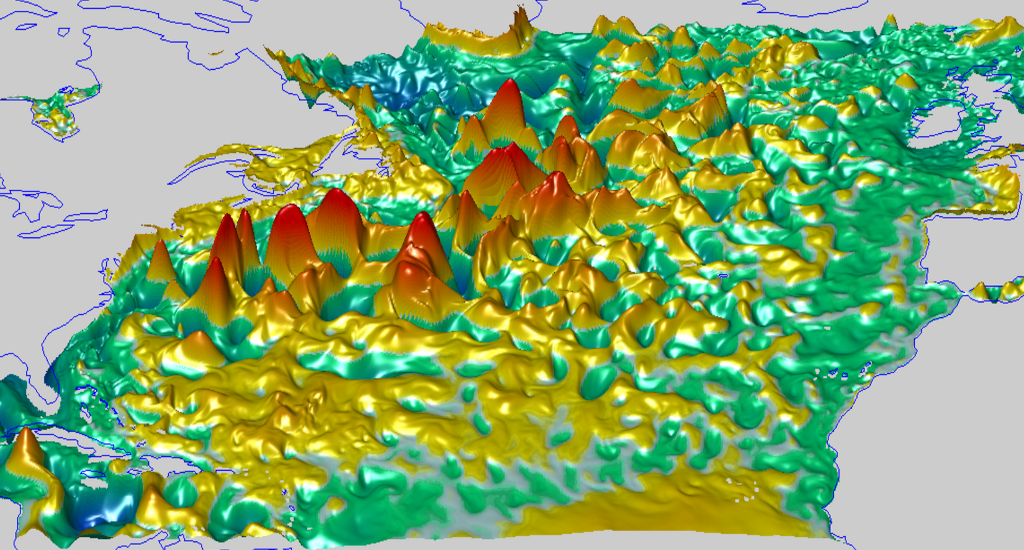
\includegraphics[width=300pt,keepaspectratio=true]{png1024x/atl1024x500PHONged.png}
%\end{figure}
%\end{frame}

%\begin{frame}
%\begin{figure}
	%\centering
	%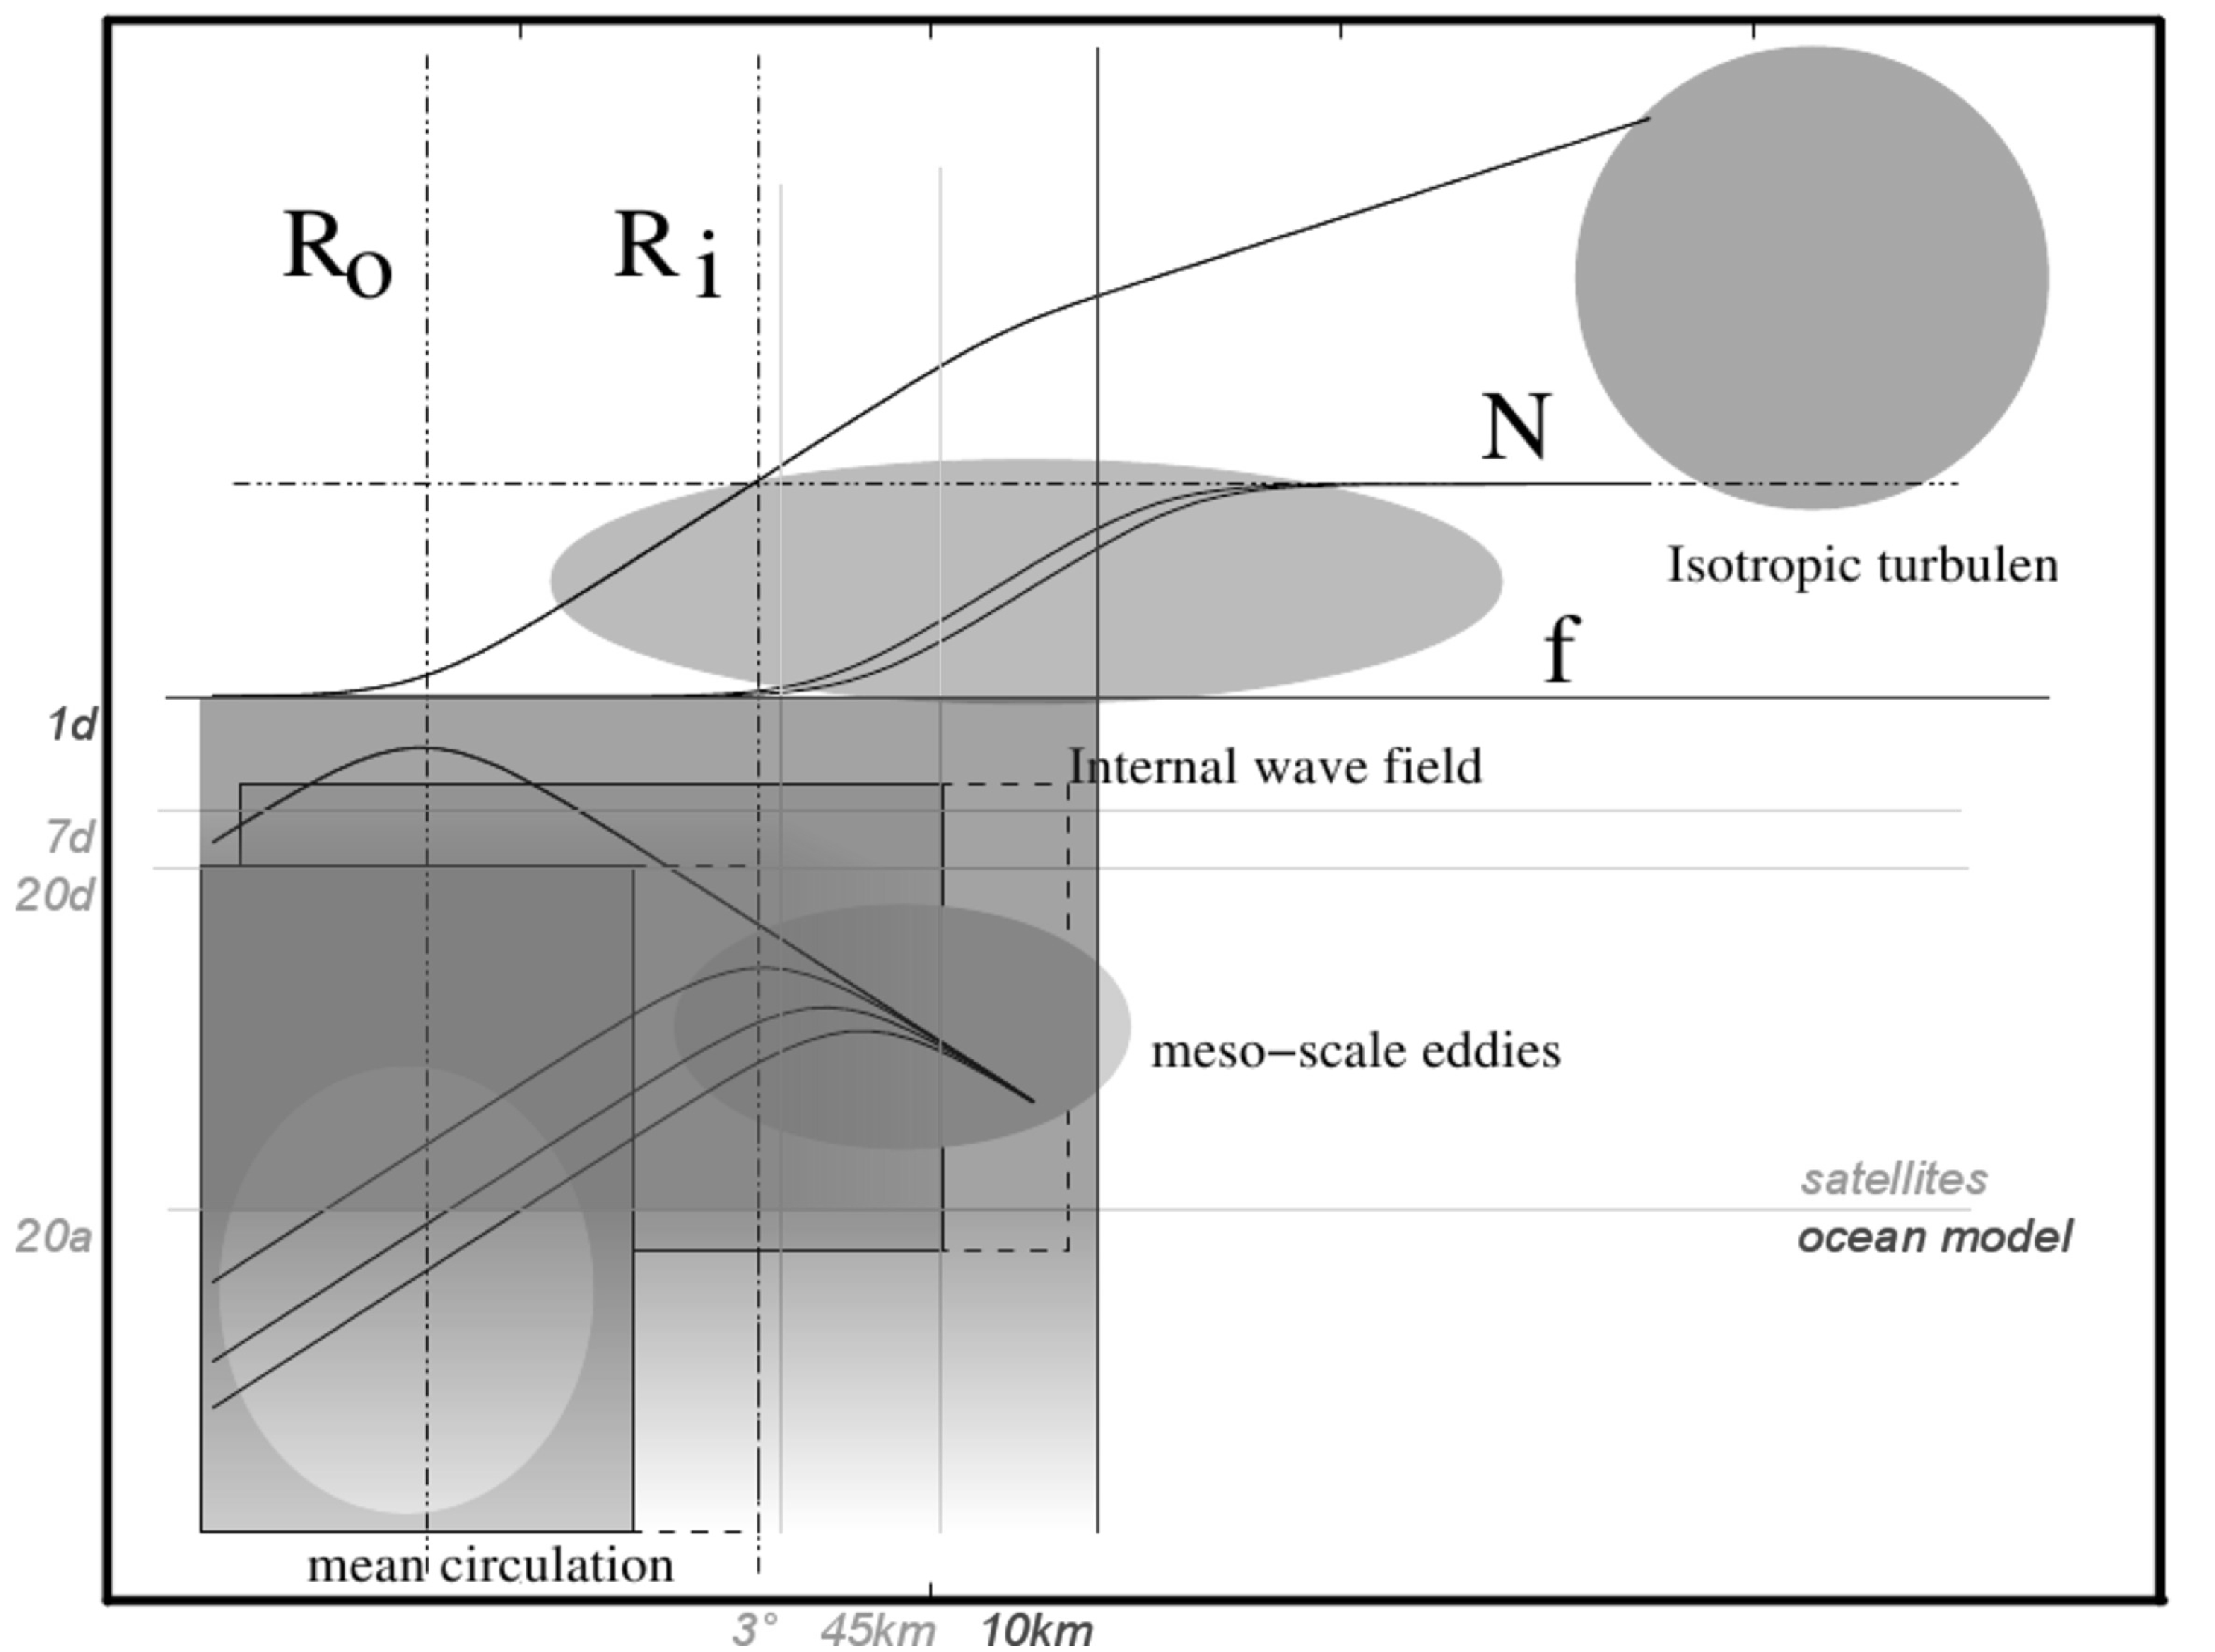
\includegraphics[width=300pt,keepaspectratio=true]{shrunks/scale_04.pdf}
%\end{figure}
%\end{frame}



% ######################################################################
\section{Teil I - Westliche Randströme}



\subsection{Analytisch}
% ######################################################################
\begin{frame}
\frametitle{Bewegunsgleichungen}
%%....................................................................
\begin{align}
	\rho \Dpr{\vec{u}}{t} 
	=
	&- 2\vec{\Omega} \times \vec{u} -\;\;\;\;\nabla p  \;\;\;\;\;\;\;\;    + \nabla \cdot\boldsymbol{\mathsf{T}}\;\;\;\; +\;\;\; \rho\vec{g} \nonumber \\
	&-      Coriolis                -    Druckgrad.+             Reibung                 +   Gravi. 
\end{align}

%%....................................................................
\begin{align}
	\Dpr{m}{t}
	&=
	0
\end{align}
%%....................................................................

%%....................................................................
\end{frame}
% ######################################################################



% ######################################################################
\begin{frame}[noframenumber]
\frametitle{Approximationen/Manipulationen}
\end{frame}
\begin{frame}
\frametitle{Approximationen/Manipulationen}
\begin{itemize}
	\item<1-> 
	mesoskalige Turbulenz parametrisiert \\
	\textit{Reynolds averaging}
	\item<2-> 
	Corioliskraft linearisiert\\
	 $\vec{f}(y) = f_{0} + \beta y$
	\item<3->
	Hydrostatische Approximation \\
	$\rho\vec{g} = -\dpr{p}{z}$ %(nur noch horizontale Kräfte übrig)
	\item<4->
	zeitlich konstant \\
	$\dpr{\vec{u}}{t} = 0$
	\item<5->
	Inkompressibiltät \\
	Massenerhaltung $\rightarrow$ Volumenerhaltung ($\rho = const$)
	\item<6->
	Horizontale Geschwindigkeiten viel größer als vertikale \\
	$w=0$
	\item<7->
	vertikal integrieren \\
	$\int_{H} \vec{u} \dint{z}=	\vec{U}$
\end{itemize}
\end{frame}
% ######################################################################

\begin{frame}
	\frametitle{Viereckiges flaches Honigbecken}
	% TODO bild aus BSC atlantic -> bild AUS BSC viereck
\end{frame}

% ######################################################################
\begin{frame}
\frametitle{übrig bleibt...}
%%....................................................................
\begin{align}
	\rho \Dpr{\vec{u}}{t} 
	=
	&- 2\vec{\Omega} \times \vec{u} -\;\;\;\;\nabla p  \;\;\;\;\;\;\;\;    + \nabla \cdot\boldsymbol{\mathsf{T}}\;\;\;\; +\;\;\; \rho\vec{g} \nonumber 
\end{align}
%%....................................................................
\begin{center}
	$\Downarrow$
\end{center}
%%....................................................................
\begin{align}
	0
	=
	%&      -f\unitvec{z} \times \vec{U}\; -    gH\grad{h} \;\;\;\;\;\;\; + \mathbf{\tau}_{s}\;\;\;\;\; - \mathbf{\tau}_{b}\;\;\;\;\;\;\;\;\;\;\;\;\; \;\;\;\; + A\grad^{2} \vec{U}  \nonumber \\
	%&-      Coriolis                -    Druckgrad.  +  Wind  - Bodenreibung  + laterale\; Reibung          \nonumber
	&  -\l f_{0} + \beta y \r \unitvec{z} \times \vec{U} -    gH\grad{h}  + \mathbf{\tau}_{s} - \mathbf{\tau}_{b}+ A\grad^{2} \vec{U} 
\end{align}
%%....................................................................
\begin{align}
	\Dpr{\vec{U}}{t}
	&=
	0
\end{align}
%%....................................................................
%%....................................................................
\end{frame}
% ######################################################################

% ######################################################################
\begin{frame}
\frametitle{Curl Operation}
%%....................................................................
\begin{align}
	0
	=&  \grad \times \left[\;\;\;\;\;   -\vec{f} \times \vec{U}   -    g H \grad{h} + \mathbf{\tau}_{s} - \mathbf{\tau}_{b} + A  \grad^{2} \vec{U} \;\;\;\;\;   \right]  \nonumber \\
     &     \nonumber 
\end{align}
%%....................................................................
\end{frame}

\begin{frame}
\frametitle{Curl Operation}
%%....................................................................
\begin{align}
	0
	=&  \grad \times \left[ \;\;\;\;\;   -\vec{f}(y) \times \vec{U}   -    g H \grad{h} + \mathbf{\tau}_{s} - \mathbf{\tau}_{b} + A  \grad^{2} \vec{U}  \;\;\;\;\;   \right]  \nonumber \\
	=& \;\;\;\;\; \;\;\; -\beta V  + \vort{\l \mathbf{\tau}_{s}- \mathbf{\tau}_{b} \r}  + A  \grad \times \grad^{2} \vec{U}    \nonumber 
\end{align}
%%....................................................................
\end{frame}
% ######################################################################

% ######################################################################
\begin{frame}
\frametitle{Stromfunktion}
%%....................................................................
\begin{align}
 \vec{U}&=\tsca{\grad} \psi(x,y) 
\end{align}
%%...................................................................
soll heißen...
%%....................................................................
\begin{align}
	U &= -\dpr{\psi}{y}  \nonumber  \\
	V &= \;\;\; \dpr{\psi}{x}   \nonumber 
\end{align}
%%....................................................................
\end{frame}
% ######################################################################

% ######################################################################
\begin{frame}
\frametitle{Stromfunktion}
%%....................................................................
\begin{align}
		0
	=& -\beta V  + \vort{\l \mathbf{\tau}_{s}- \mathbf{\tau}_{b} \r}  + A  \grad \times \grad^{2} \vec{U}    \nonumber 
\end{align}
%%....................................................................
%\begin{center}
	%$\Downarrow$
%\end{center}
%%%....................................................................
%\begin{align}
		%0
	%=& -\beta \dpr{\psi}{x}  + \vort{\l \mathbf{\tau}_{s}- \mathbf{\tau}_{b} \r}  + A  \grad \times \grad^{2} \gradt \psi   \nonumber 
%\end{align}
%%%....................................................................
\begin{center}
	$\Downarrow$
\end{center}
%%....................................................................
\begin{align}
		0
	=& -\beta \dpr{\psi}{x}  + \vort{\l \mathbf{\tau}_{s}- \mathbf{\tau}_{b} \r}  + A  \grad^{4} \psi  
\end{align}
%%....................................................................
\end{frame}
% ######################################################################

% ######################################################################
\begin{frame}
\frametitle{weitere Approximationen}
\begin{itemize}
	\item<1-> 
	Bodenreibung proportional zu $\vec{U}$ \\
	$\vec{\tau_b} = R \vec{U}$
	\item<2->
	keine laterale Reibung! \\
	$A  \grad^{4} \psi  = 0 $
	\item<3->
	Windstress sinusoidale Funktion von $y$ \\
	$\vec{\tau_s} = F \cos{(\pi y / B)}$	
\end{itemize}
\end{frame}
% ######################################################################

% ######################################################################
\begin{frame}
\frametitle{weitere Approximationen}
%%....................................................................
\begin{align}
		0
	=& -\beta \dpr{\psi}{x}  + \vort{\l \mathbf{\tau}_{s}- \mathbf{\tau}_{b} \r}  + A  \grad^{4} \psi \nonumber  
\end{align}
%%....................................................................
\begin{center}
	$\Downarrow$
\end{center}
%%....................................................................
\begin{align}
		0
	=& -\beta \dpr{\psi}{x}  - R \vort{U} - F \grad \times  \cos{(\pi y / B)} \nonumber   \\
	%=& -\beta \dpr{\psi}{x}  - R \grad^2 \psi+ F \dpr{}{y} \cos{(\pi y / B)}  \nonumber  \\
	=& -\beta \dpr{\psi}{x}  - R \grad^2 \psi + \frac{F\pi}{B} \sin{(\pi y / B)}\nonumber  \\
R \grad^2 \psi+\beta \dpr{\psi}{x}   
	=&
	 F\alpha \sin{(\alpha y )}
\end{align}
%%....................................................................
...mit $ \alpha	= \frac{\pi}{B} $
\end{frame}
% ######################################################################

% ######################################################################
\begin{frame}
\frametitle{Analytische Lösung möglich}
Inhomogene partielle Differentialgleichung 2er Ordnung.
%%....................................................................
\begin{align}
    R \grad^2 \psi+\beta \dpr{\psi}{x}   
	=&
	 F\alpha \sin{(\alpha y )}\nonumber 
\end{align}
%%....................................................................
% TODO analy loesung zeigen
% TODO bild!
\end{frame}
% ######################################################################

% ######################################################################
\begin{frame}
\frametitle{Numerische Lösung}
\begin{itemize}
	\item
	variable Beckenform
	\item
	variabler Windstress
\end{itemize}
%%....................................................................
\begin{align}
    R \grad^2 \psi+\beta \dpr{\psi}{x}   
	=&
	 W(x,y)
\end{align}
%%....................................................................
% TODO bild!
\end{frame}
% ######################################################################

% ######################################################################
\begin{frame}
\frametitle{Jacobi-Methode}
Annahme: $\psi^{k=1}=rand$ überall
%%....................................................................
\begin{align}
    R \grad^2 \psi^k_{i,j} + \beta \dpr{}{x}\psi^k_{i,j} - W_{i,j}
    &=
    \Phi_{i,j}
\end{align}
%%....................................................................

%%....................................................................
\begin{align}
    R \grad^2 \psi^{k+1}_{i,j} + \beta \dpr{}{x} \psi^{k+1}_{i,j} - W_{i,j}
    &=
   0
\end{align}
%%....................................................................
\end{frame}
% ######################################################################







\subsection{Numerisch}

% ######################################################################
\begin{frame}
\frametitle{Numerische Lösung}
\begin{itemize}
	\item
	variable Beckenform
	\item
	variabler Windstress
\end{itemize}
% TODO bild!
\end{frame}
% ######################################################################


% ######################################################################
\begin{frame}
\frametitle{Finite Differenzen}
 TODO bild aus BSC gitter!
  \end{frame}
% ######################################################################

% ######################################################################
\begin{frame}
\frametitle{Finite Differenzen}
 Beispiel $\dpr{\psi(x)}{x}$ durch Taylorreihe diskretisiert:
 %%....................................................................
 \begin{align} \label{tayA}
	\psi(x + \delta x)
	&=
	\psi(x)
	+ \frac{\delta x}{1!} \dpr{\psi}{x}
	+ \frac{\delta x^2}{2!} \dpr{^2\psi}{x^2}
	+ ...
 \end{align}
 %%....................................................................
 %%....................................................................
 \begin{align} \label{tayB}
	\psi(x - \delta x)
	&=
	\psi(x)
	- \frac{\delta x}{1!} \dpr{\psi}{x}
	+ \frac{\delta x^2}{2!} \dpr{^2\psi}{x^2}
	+ ...
 \end{align}
 %%....................................................................
 \pause
 \eqref{tayA} - \eqref{tayB}:
 %%....................................................................
 \begin{align}
	\dpr{\psi}{x}
	&\approx
	\frac{\psi(x + \delta x) - 	\psi(x - \delta x)}{2 \delta x} \nonumber
 \end{align}
 %%.................................................................... 
 \end{frame}
% ######################################################################

\begin{frame}
	\frametitle{Höhere Ordnungen}
	Beispiel: $\grad^2$ an der Stelle $(0,0)$
	%%....................................................................
	\begin{align}
		&\grad^2 \psi(0,0)
		=
		 \dpr{^2 \psi}{x^2} + \dpr{^2 \psi}{ y^2} \nonumber\\
		&\approx
		\frac{\psi(1,0) - 2 \psi(0,0) + \psi(-1,0)}{\delta x^2}
		+
		\frac{\psi(0,1) - 2 \psi(0,0) + \psi(0,-1)}{\delta y^2}\nonumber
	\end{align}
	%%....................................................................
\end{frame}

% ######################################################################
\begin{frame}
\frametitle{Numerische Lösung}
\begin{align}
    R \grad^2 \psi  +  \beta \dpr{\psi}{x}\nonumber
	=&
	 W(x,y)
\end{align}
...erst mal ohne $\beta \dpr{\psi}{x}$
\pause
%%....................................................................
\begin{align}
    \grad^2 \psi
	=&
	 W(x,y)\nonumber
\end{align}
%%....................................................................
\pause
mit Randbedingung (willkürlich)
%%....................................................................
\begin{align}
	\psi_{bndry} = 0	\nonumber
\end{align}
%%....................................................................
% TODO bild!
\end{frame}
% ######################################################################


% ######################################################################
\begin{frame}
\frametitle{Jacobi-Methode}
\textit{first guess}: $\psi^{k=0}=random$ \\
%%....................................................................
\begin{align}
     \grad^2 \psi^k_{i,j} 
    &=
     W_{i,j} \nonumber
\end{align}
\pause
$k$:
\begin{align}
     \grad^2 \psi^k_{i,j}  - W_{i,j}
    &=
    \Phi_{i,j} \label{k0}
\end{align}
%%....................................................................
\pause
$k+1$:
%%....................................................................
\begin{align}
     \grad^2 \psi^{k+1}_{i,j}  - W_{i,j}
    &=
   0 \label{k1}
\end{align}
%%....................................................................
\end{frame}
% ######################################################################

% ######################################################################
\begin{frame}
\frametitle{Jacobi-Methode}
\eqref{k1} - \eqref{k0}:
%%....................................................................
\begin{align}
	\grad^2 \psi^{k+1}_{i,j} - \grad^2 \psi^{k}_{i,j}
    &=
    -\Phi_{i,j} 	
\end{align}
%%....................................................................
\end{frame}
% ######################################################################

% ######################################################################
\begin{frame}
\frametitle{Jacobi-Methode}
einsetzen :
%%....................................................................
\begin{align}
	\frac{\psi^{k}_{i+1,j} - 2 \psi^{k+1}_{i,j} + \psi^{k}_{i-1,j}}{\delta x^2}
-
	\frac{\psi^{k}_{i+1,j} - 2 \psi^{k  }_{i,j} + \psi^{k}_{i-1,j}}{\delta x^2}
+ \mathit{term_y}
    &=
    -\Phi_{i,j} 	\nonumber
\end{align}
\pause
\begin{align}
	   \psi^{k+1}_{i,j}      
    &=
	\frac{\delta x}{2}\Phi_{i,j} +  \psi^{k}_{i,j}  	\nonumber
\end{align}
%%....................................................................
\end{frame}
% ######################################################################

% ######################################################################


% ######################################################################
\section{Teil II - Geostrophische Ozeanwirbel}
%\begin{frame}[]
\frametitle{}
\begin{figure}
	\centering
	\includegraphics[height=200pt,keepaspectratio=true]{boundCurrs.pdf}
\end{figure}
\end{frame}
 TODO global bild
\subsection{Was ist ein \protect\textit{Eddy}?}
a


\subsection{\protect\textit{detection and tracking}-Algorithmus}
a

% ######################################################################




%\section{Methods}
%\subsection{Detection}
%\begin{frame}
\frametitle{SSH-based detection}
\begin{figure}
	\centering
% 	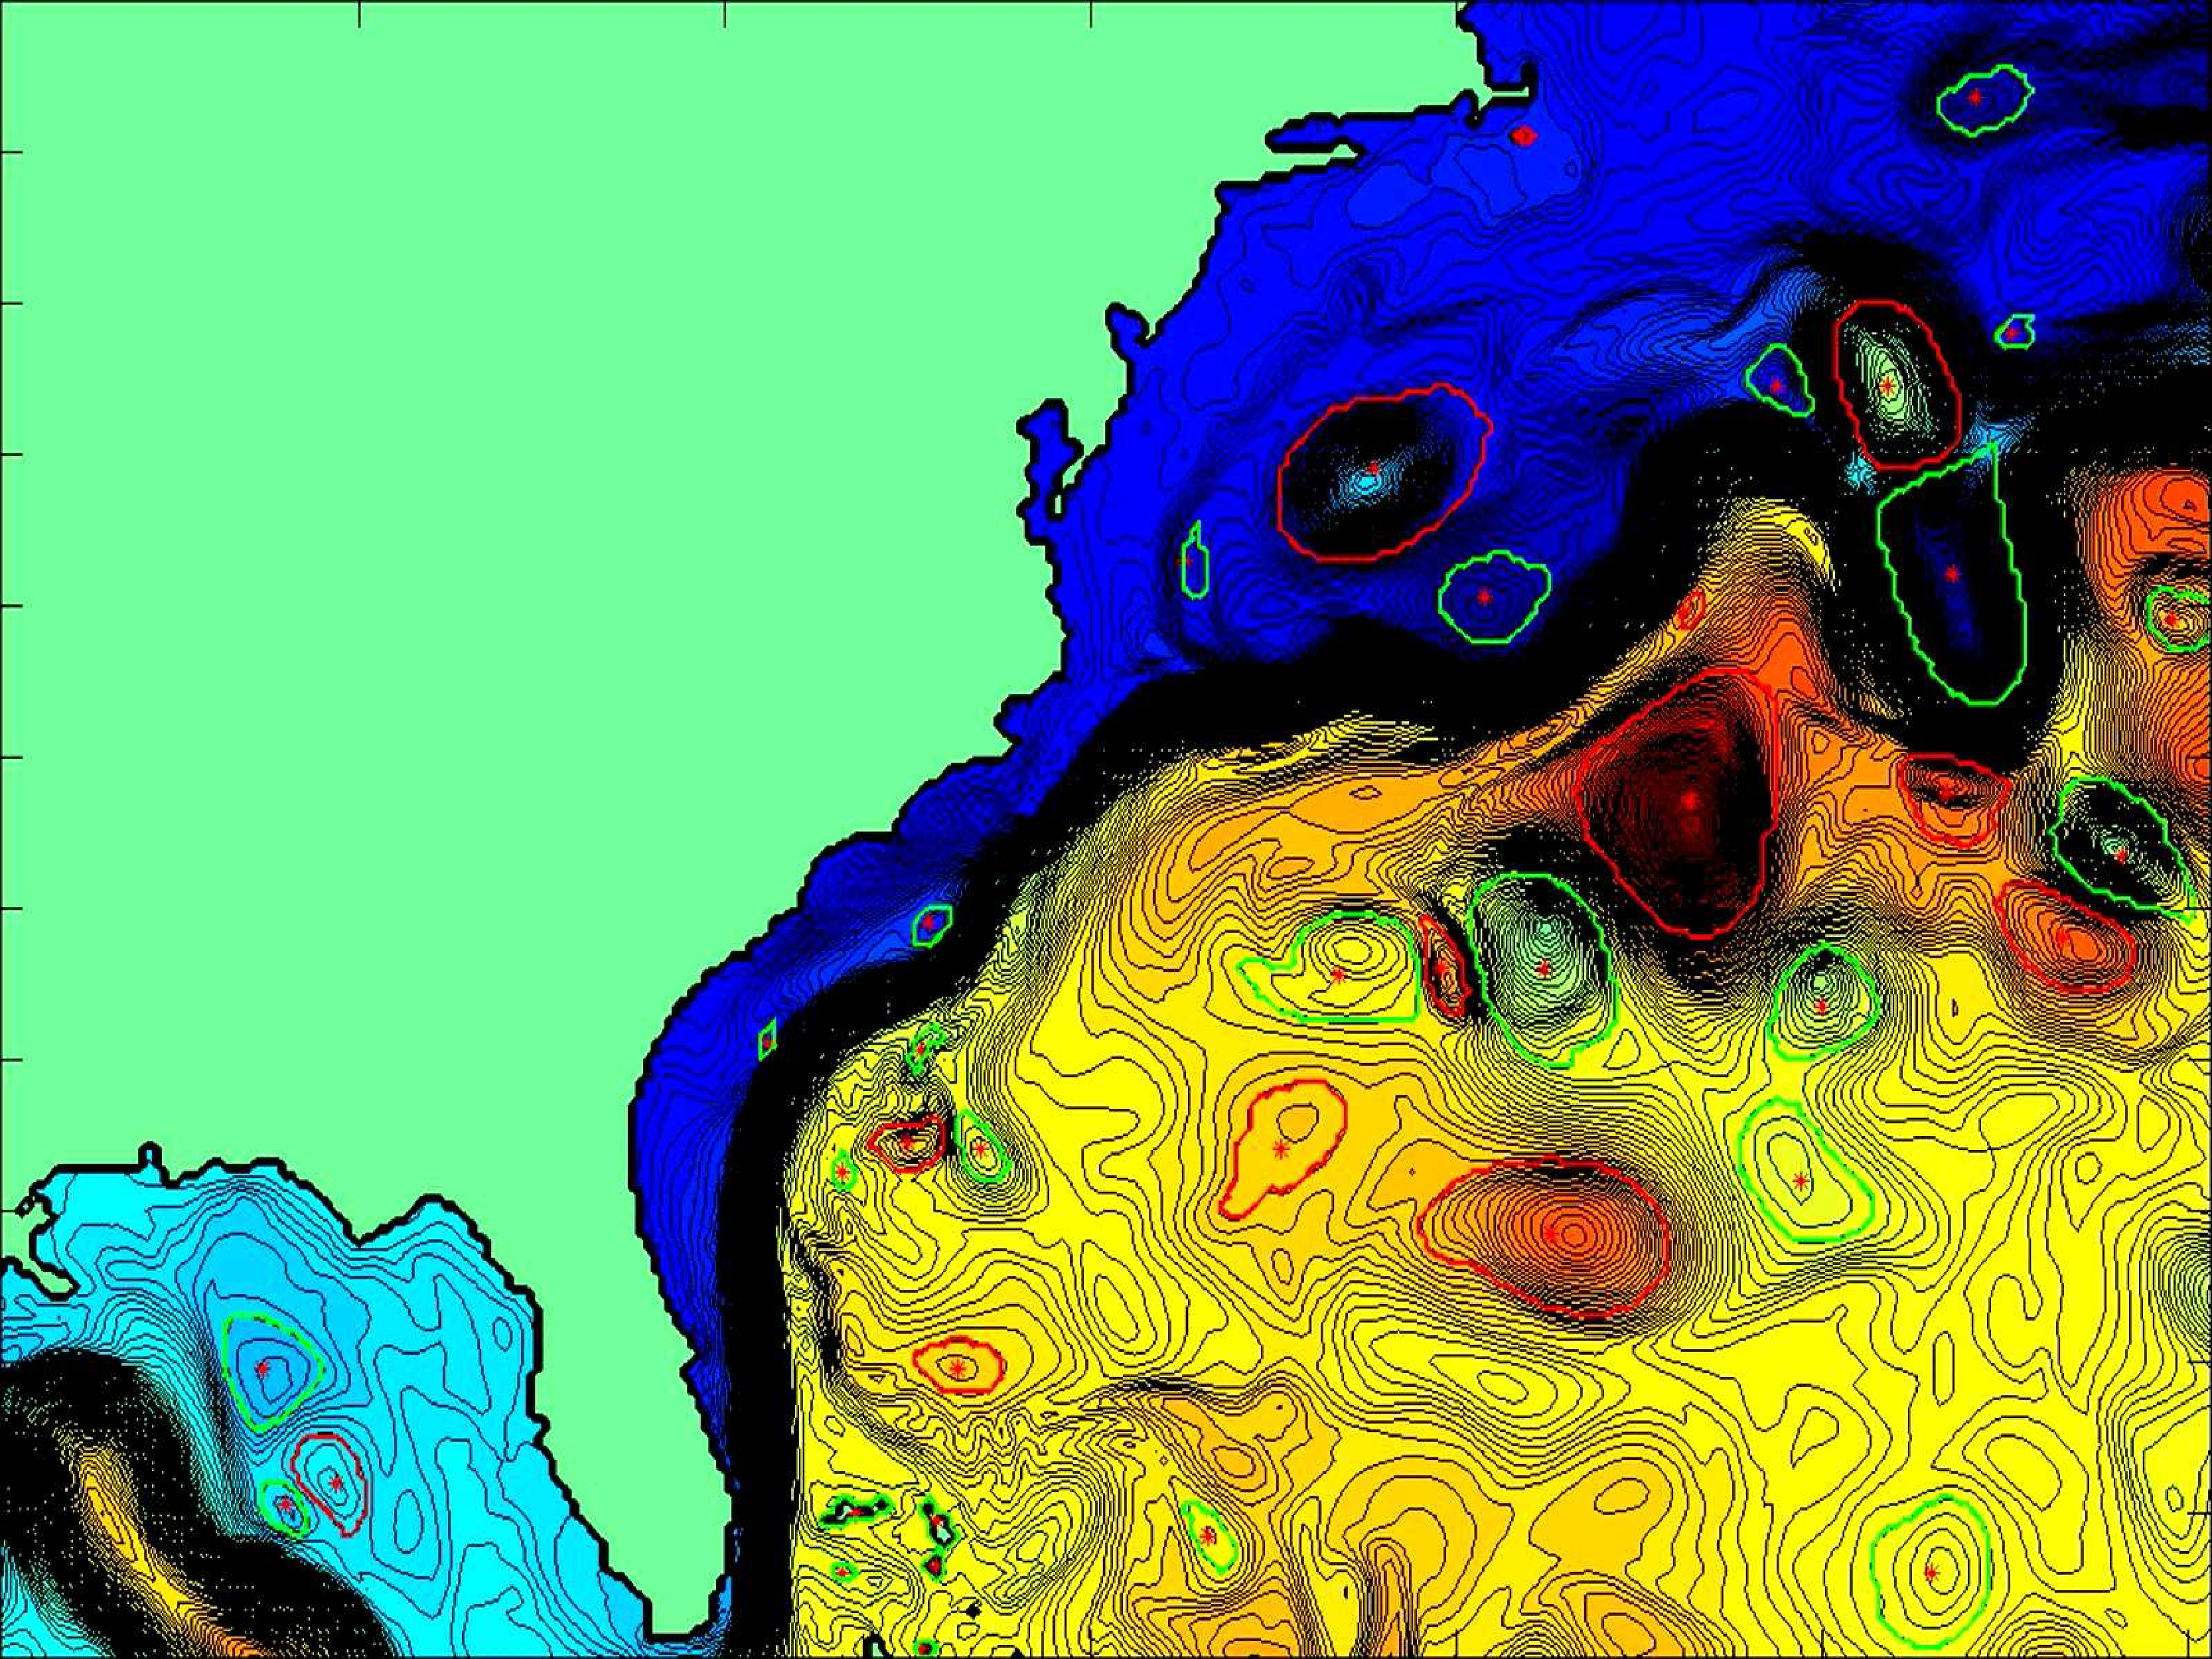
\includegraphics[width=300pt,keepaspectratio=true]{GS.pdf}
	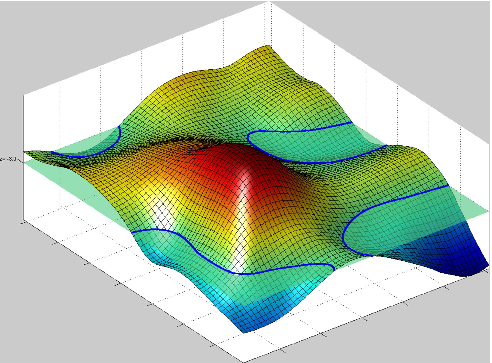
\includegraphics[height=200pt,keepaspectratio=true]{shrunks/slice1.pdf}
\end{figure}
\end{frame}

\begin{frame}[noframenumbering]
\frametitle{SSH-based detection}
\begin{figure}
	\centering
% 	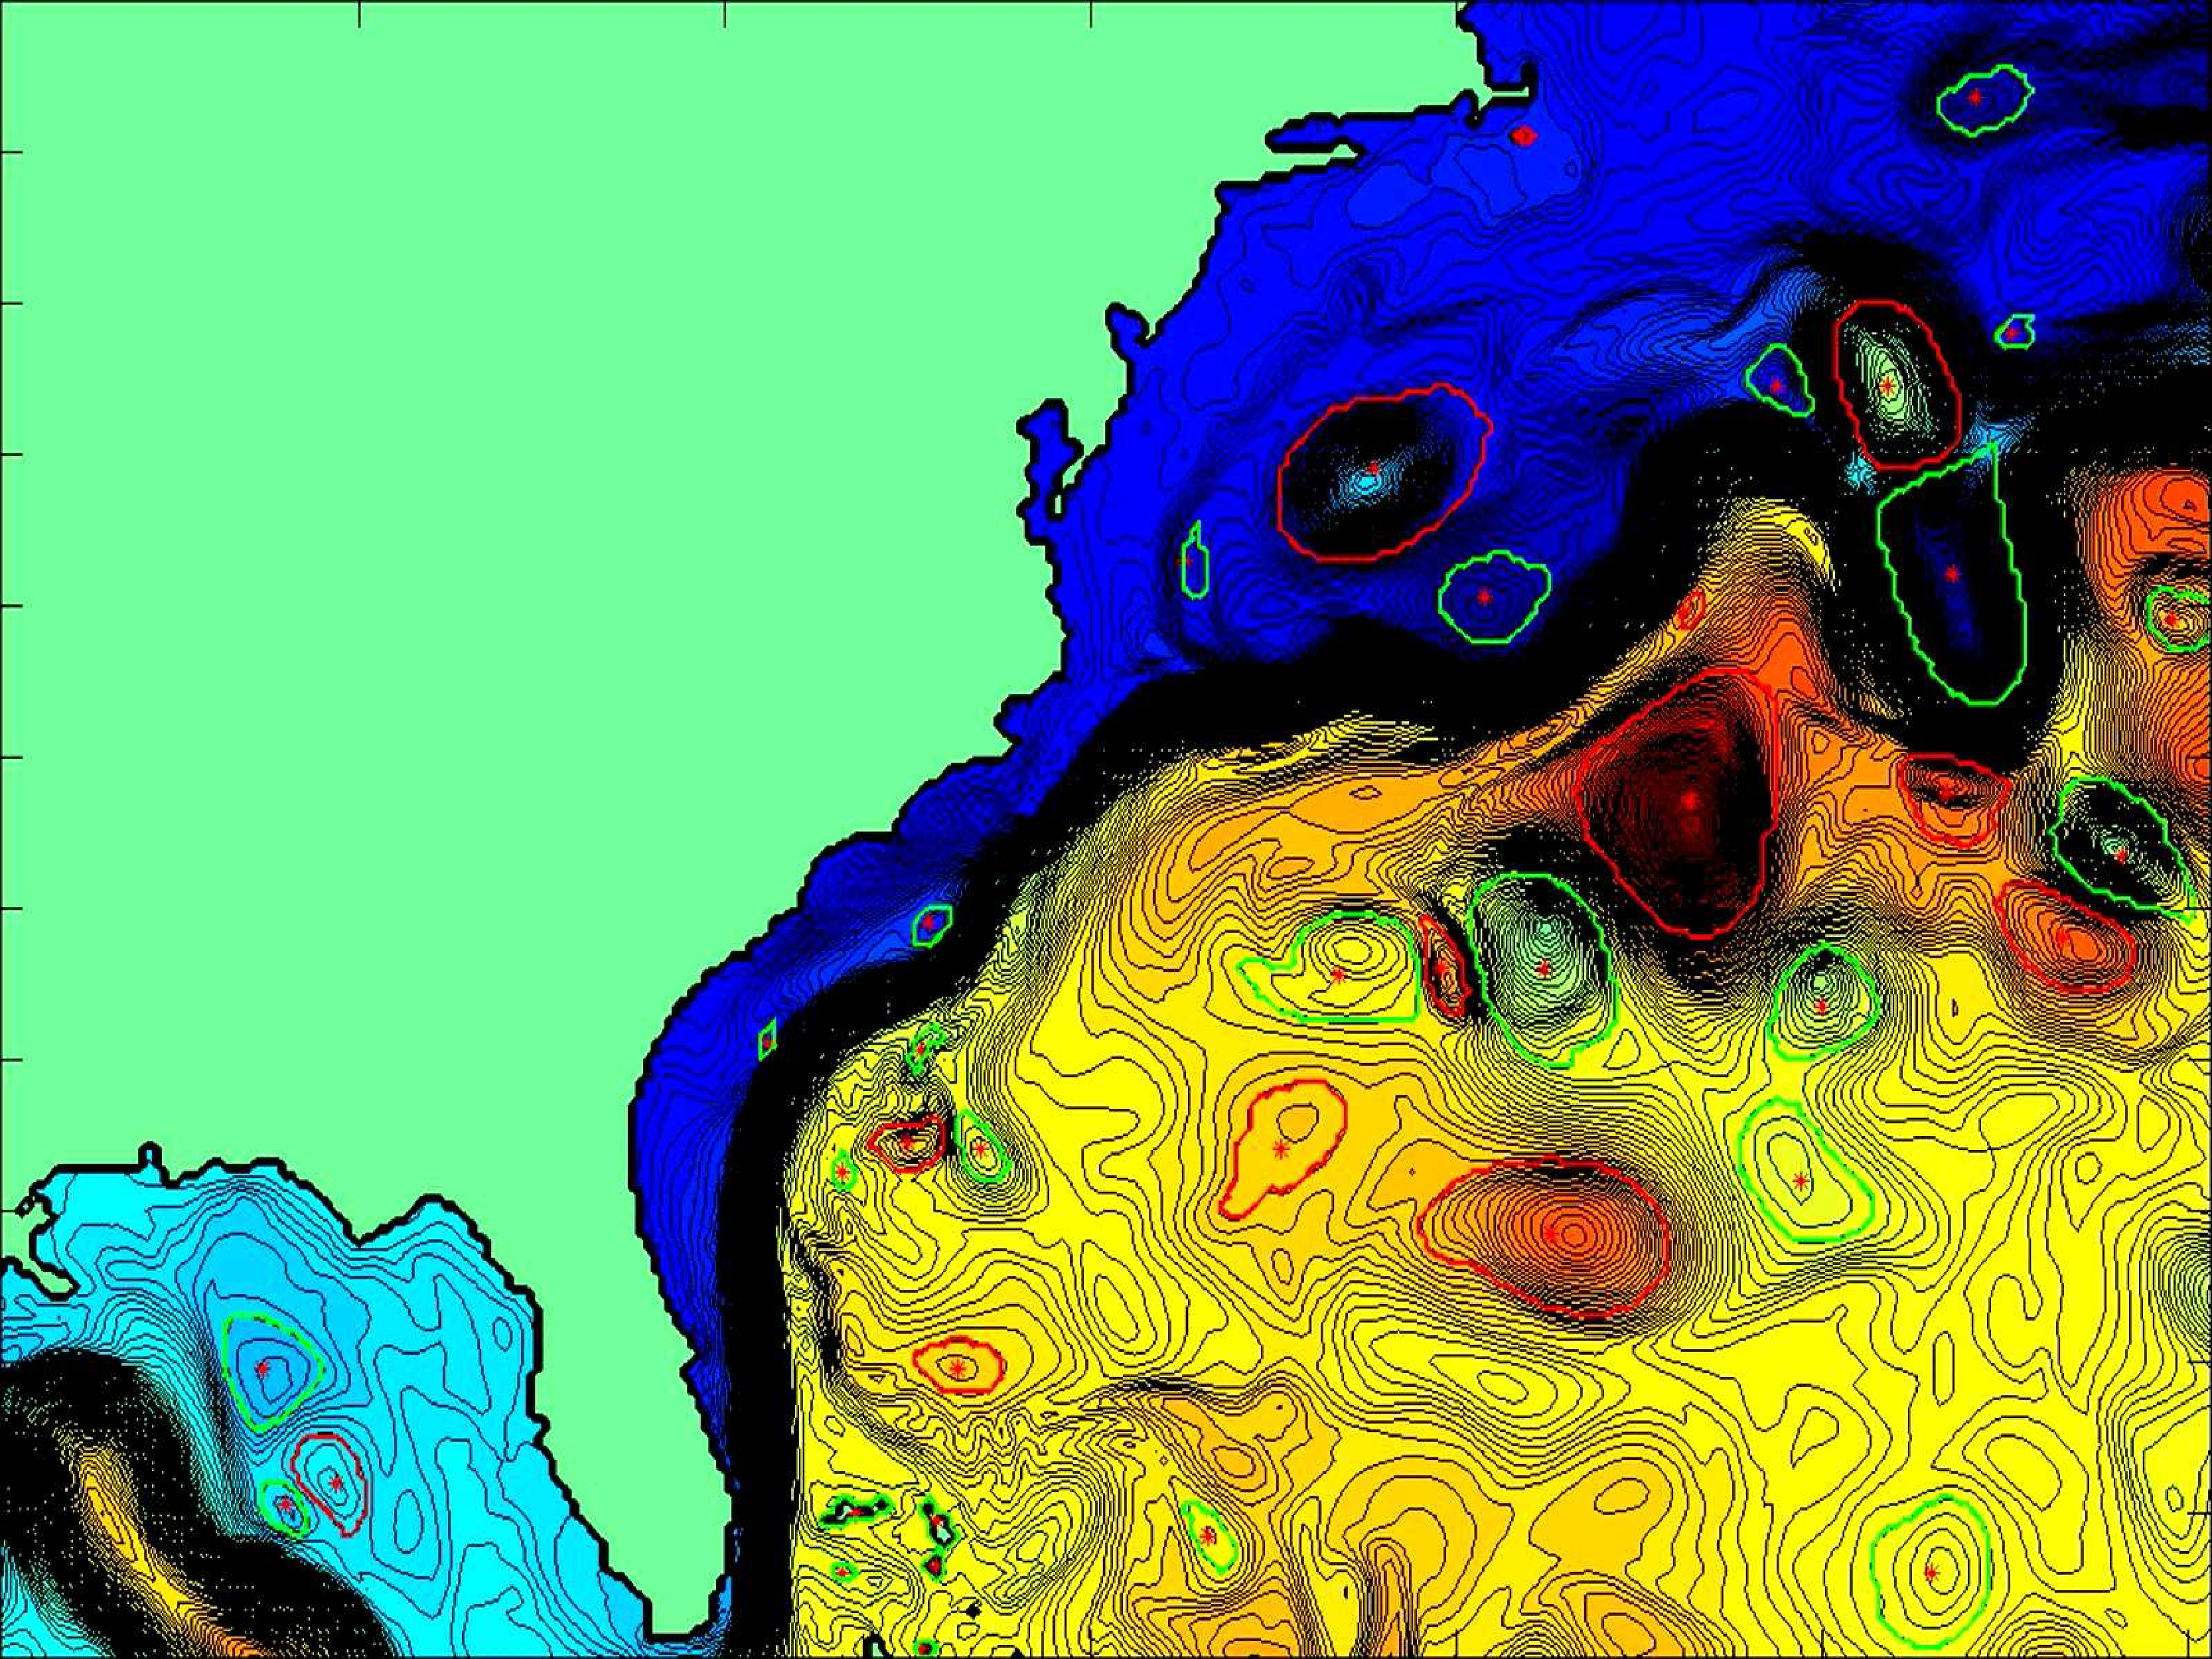
\includegraphics[width=300pt,keepaspectratio=true]{GS.pdf}
	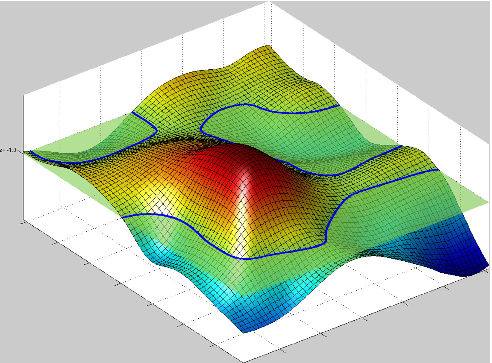
\includegraphics[height=200pt,keepaspectratio=true]{shrunks/slice2.pdf}
\end{figure}
\end{frame}

\begin{frame}[noframenumbering]
\frametitle{SSH-based detection}
\begin{figure}
	\centering
% 	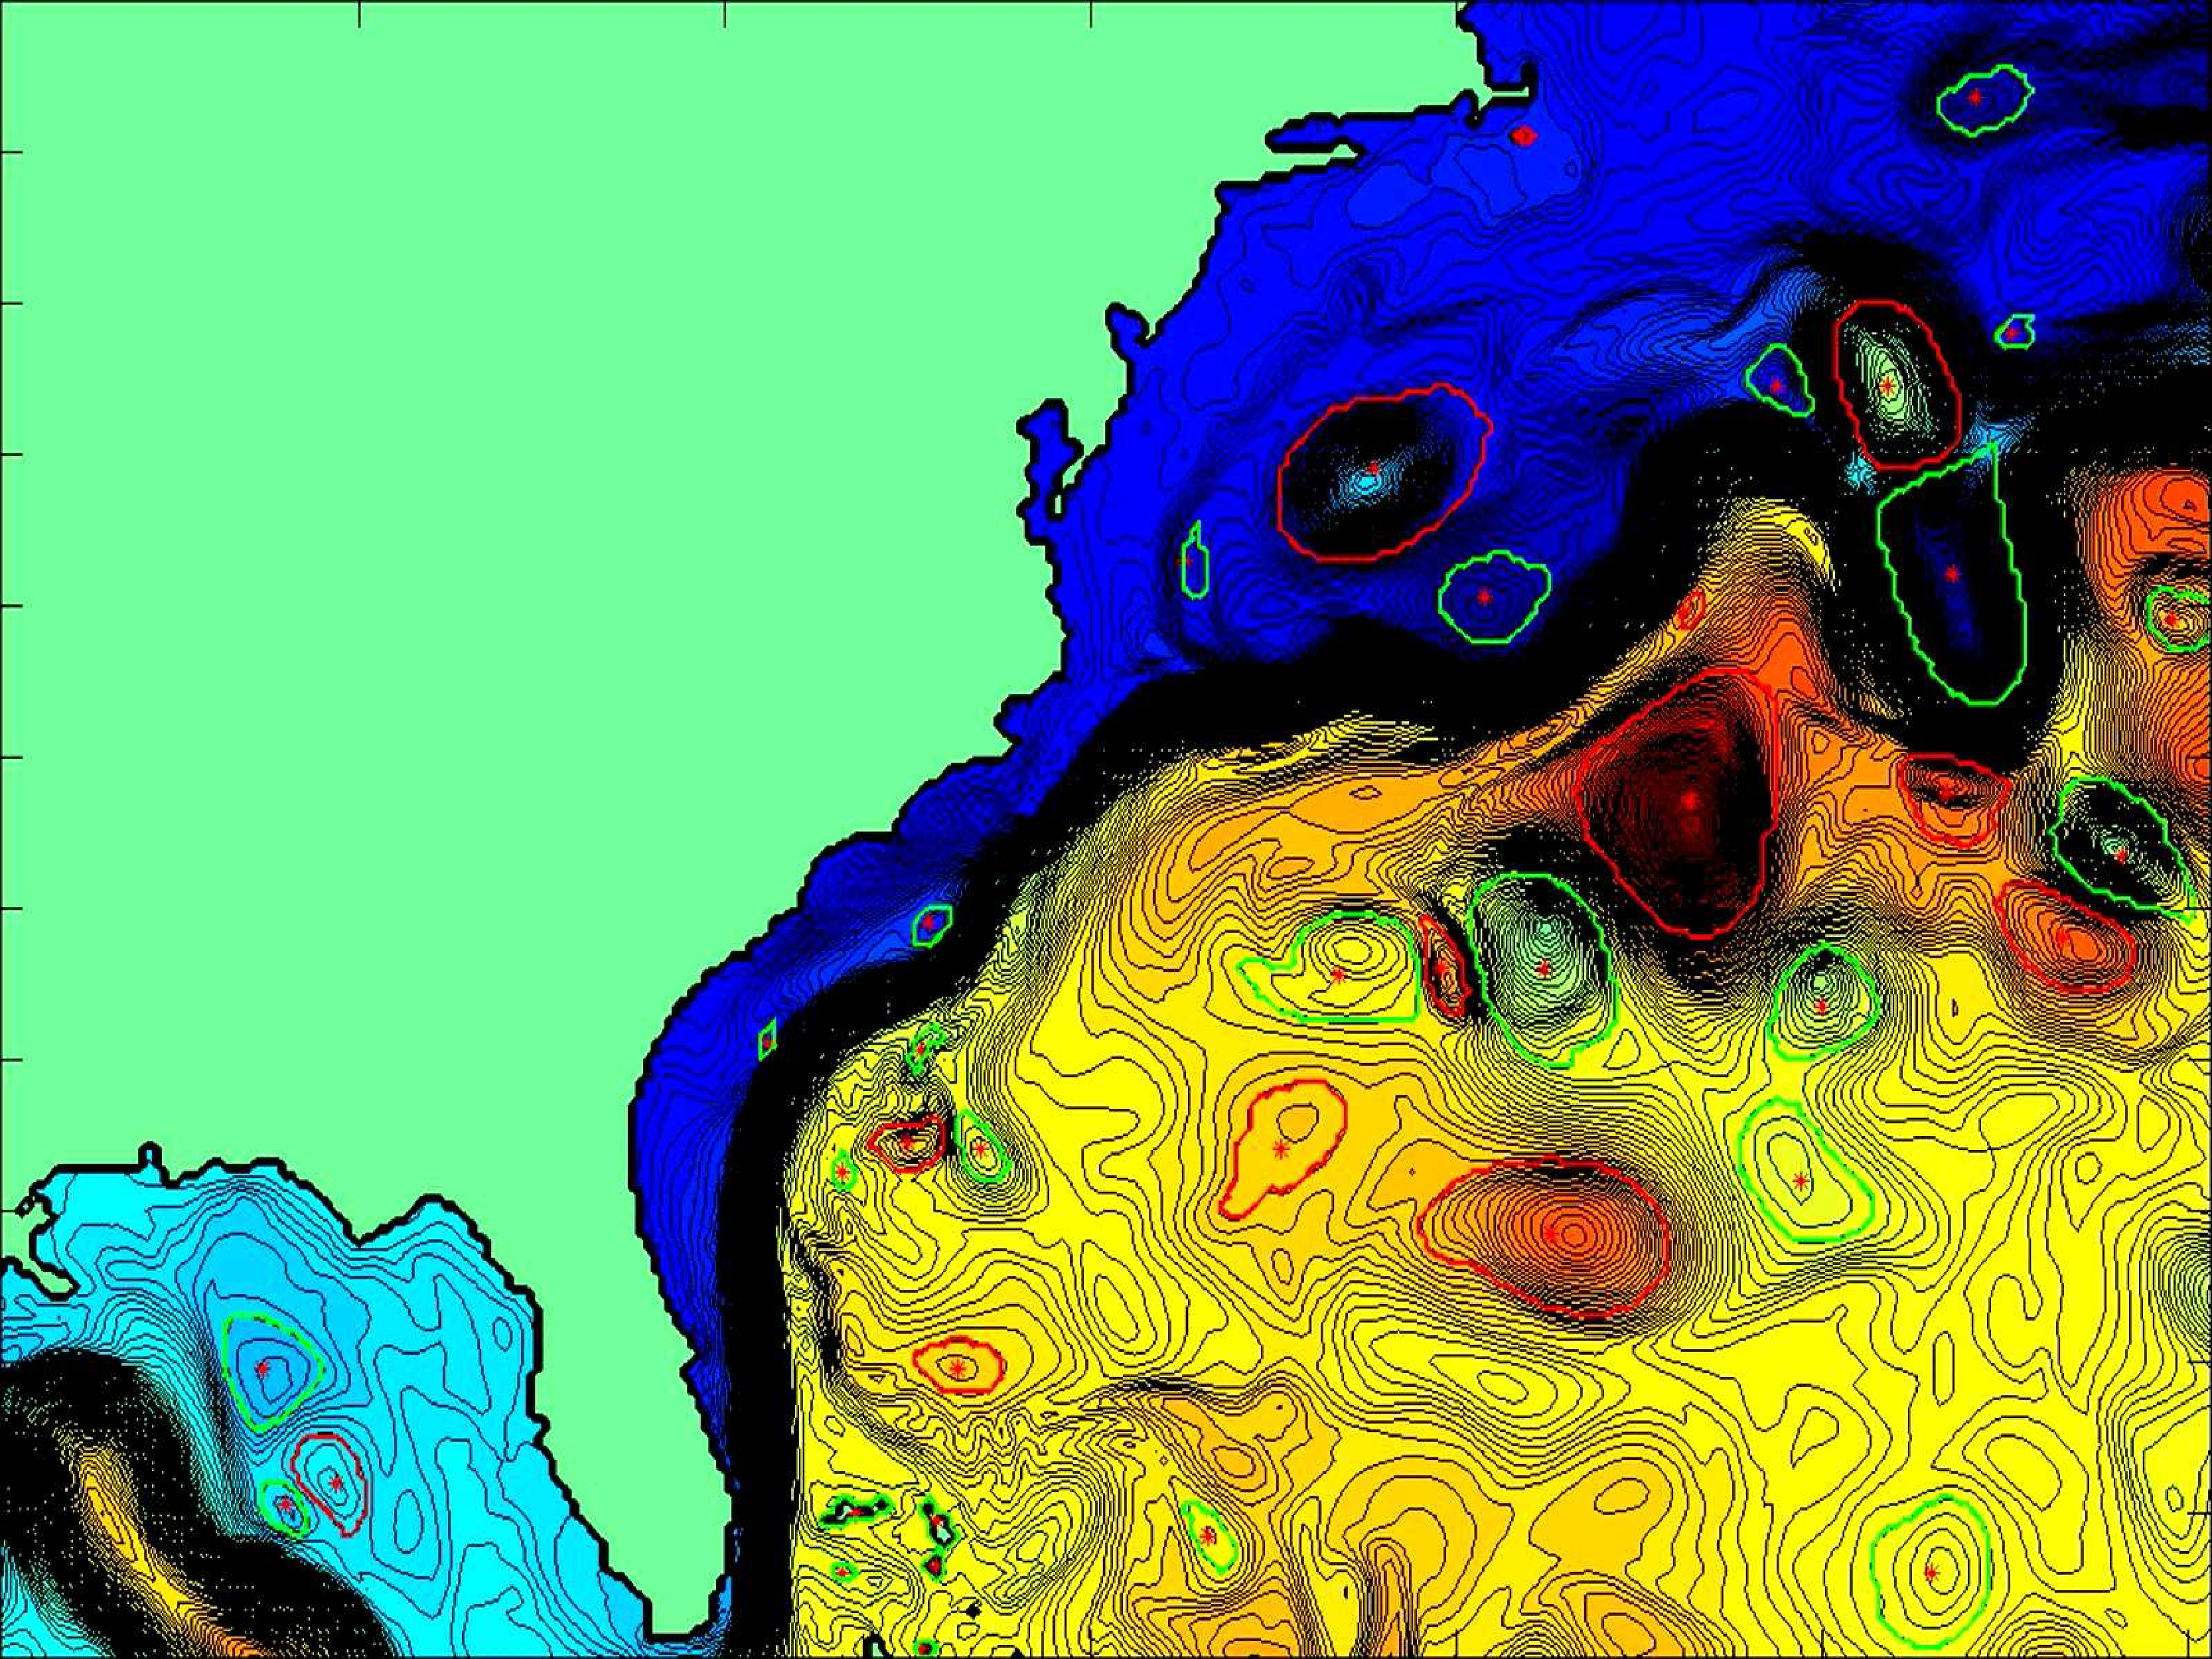
\includegraphics[width=300pt,keepaspectratio=true]{GS.pdf}
	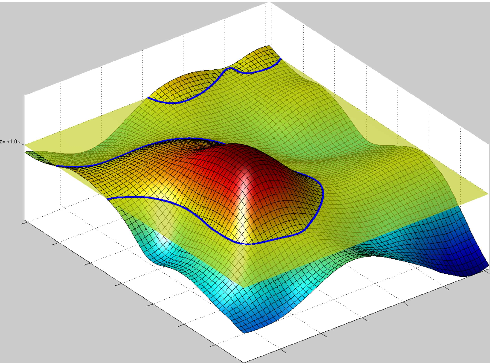
\includegraphics[height=200pt,keepaspectratio=true]{shrunks/slice3.pdf}
\end{figure}
\end{frame}

\begin{frame}[noframenumbering]
\frametitle{SSH-based detection}
\begin{figure}
	\centering
% 	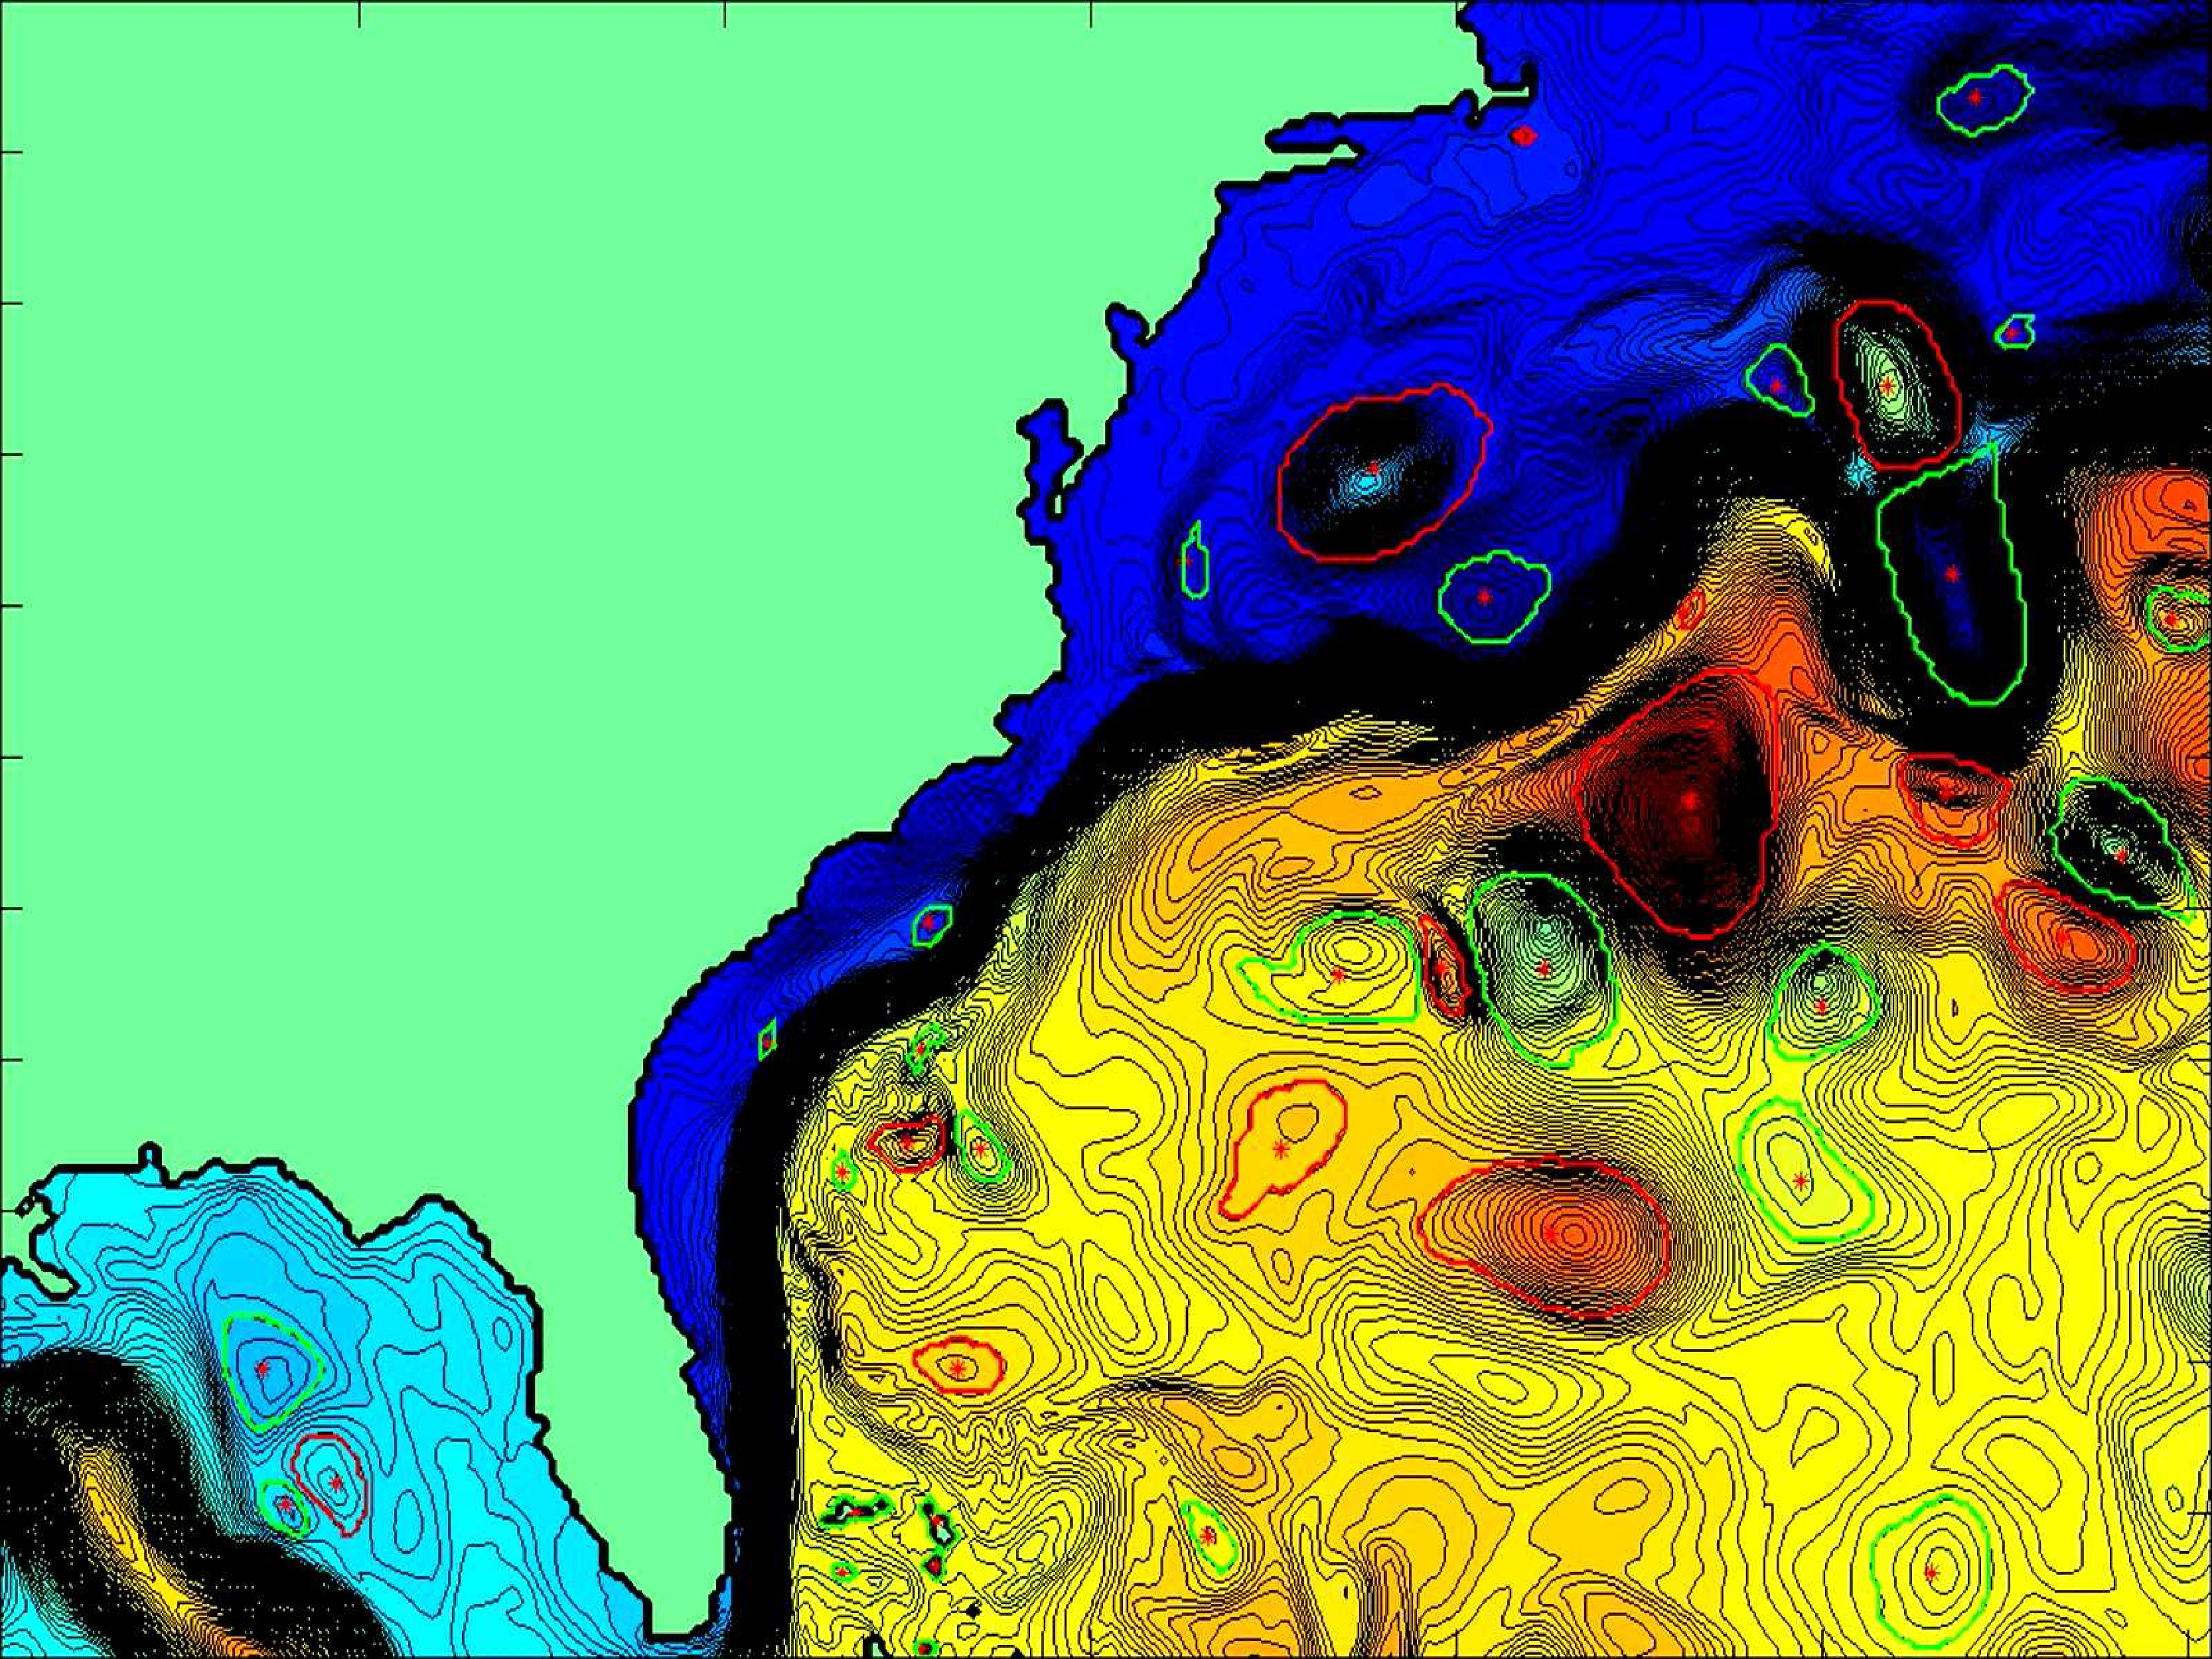
\includegraphics[width=300pt,keepaspectratio=true]{GS.pdf}
	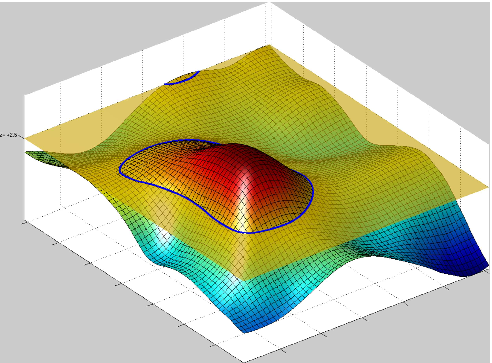
\includegraphics[height=200pt,keepaspectratio=true]{shrunks/slice4.pdf}
\end{figure}
\end{frame}

%\begin{frame}[noframenumbering]
%% \frametitle{pictures in latex beamer class}
%\begin{figure}
	%\centering
%% 	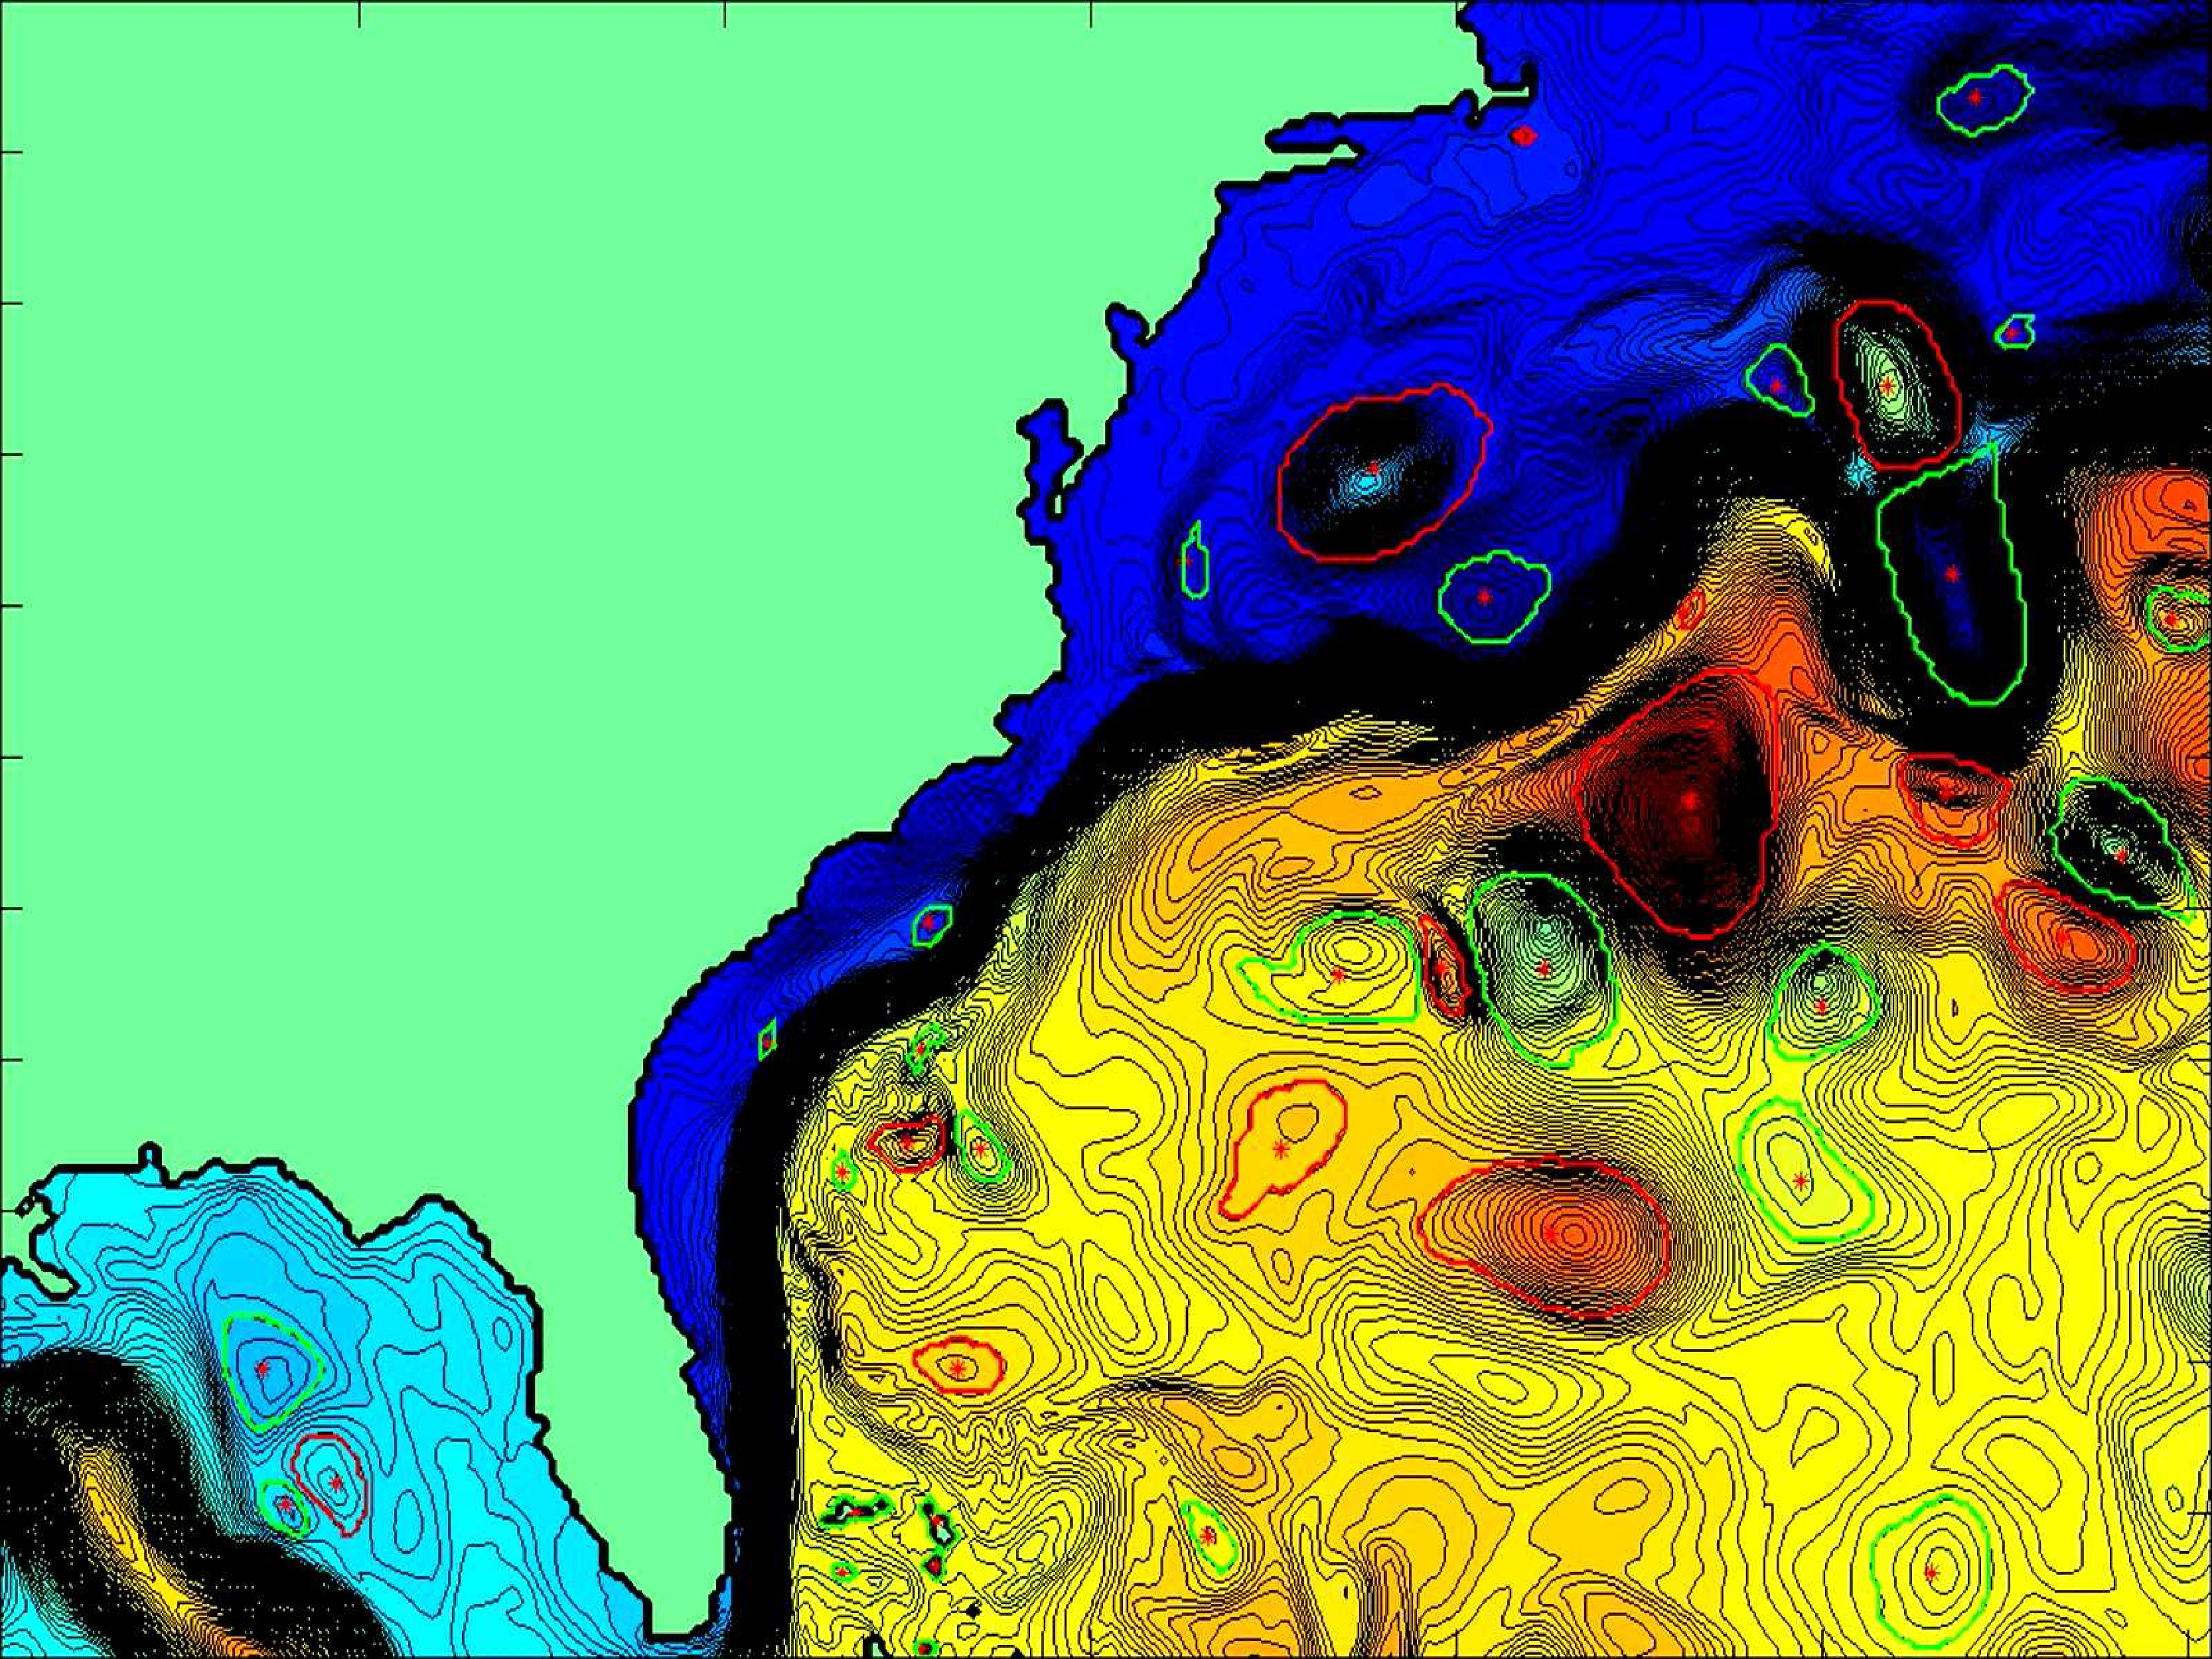
\includegraphics[width=300pt,keepaspectratio=true]{GS.pdf}
	%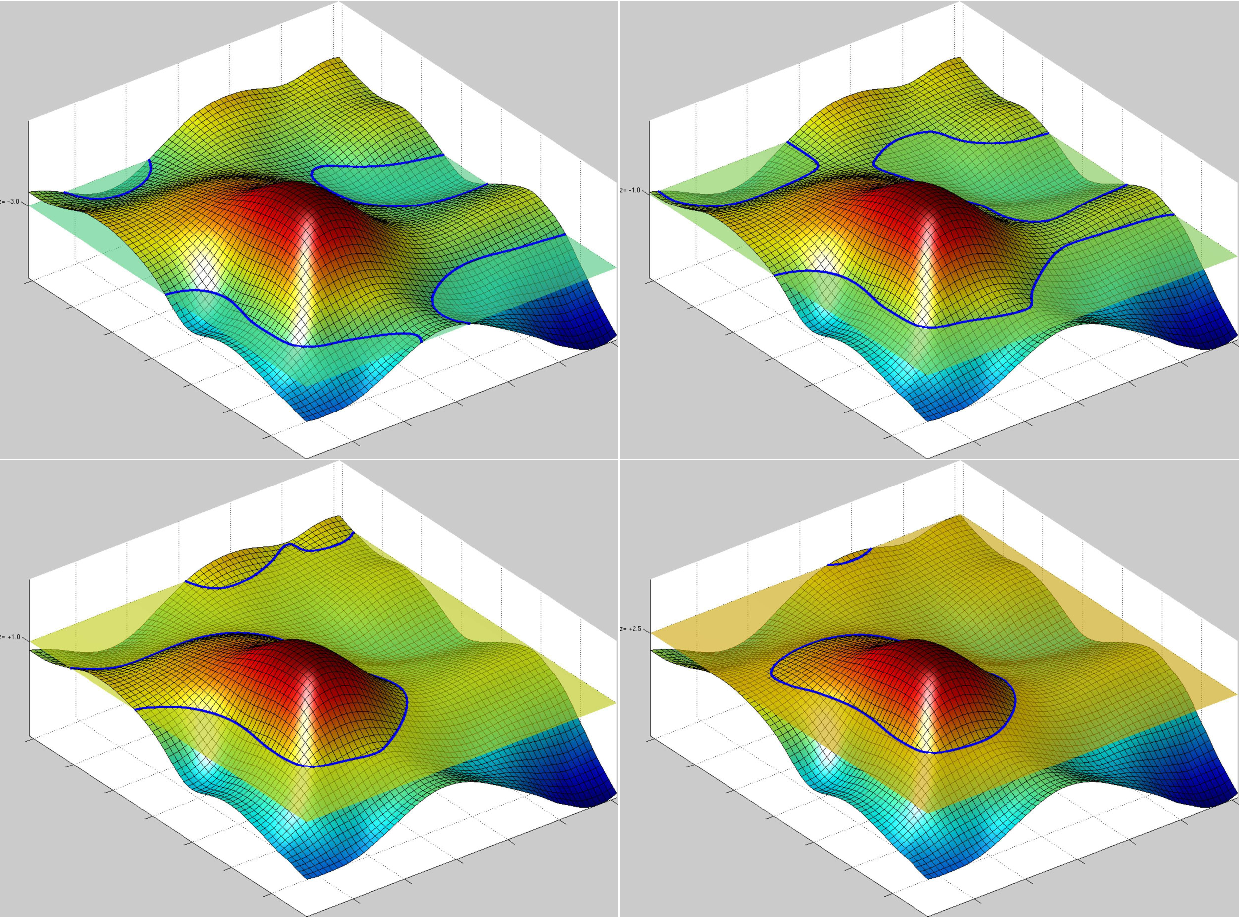
\includegraphics[height=200pt,keepaspectratio=true]{shrunks/sliceAll.pdf}
%\end{figure}
%\end{frame}

\begin{frame}
 \frametitle{does found contour qualify?}
\begin{figure}
	\begin{centering}
	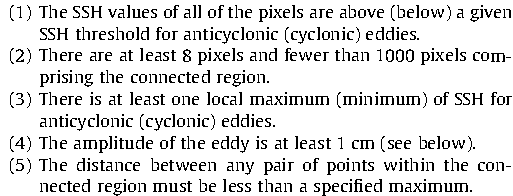
\includegraphics[width=.5\textwidth]{cheltCritsVerbatim.pdf}%
	\end{centering}
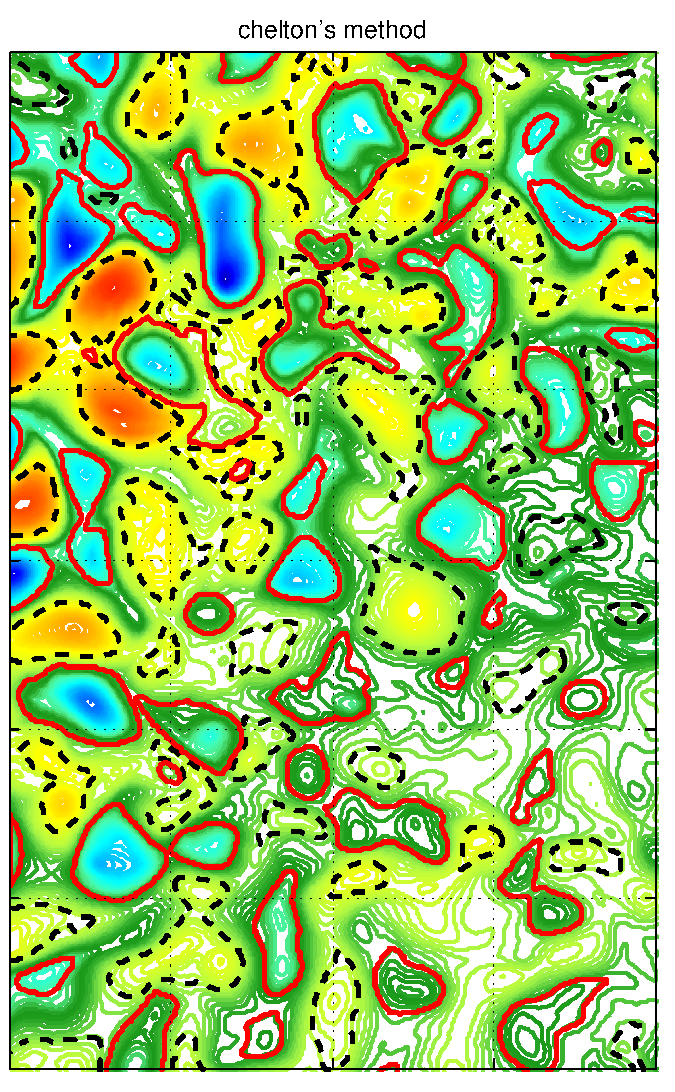
\includegraphics[height=200pt]{shrunks/ch.pdf}
\end{figure}
\end{frame}

\begin{frame}
 \frametitle{new approach: demand circular shapes}
\begin{figure}
%\includemovie{1cm}{1cm}{FIGS/Rotational_vortex.gif}
	\centering	
% 	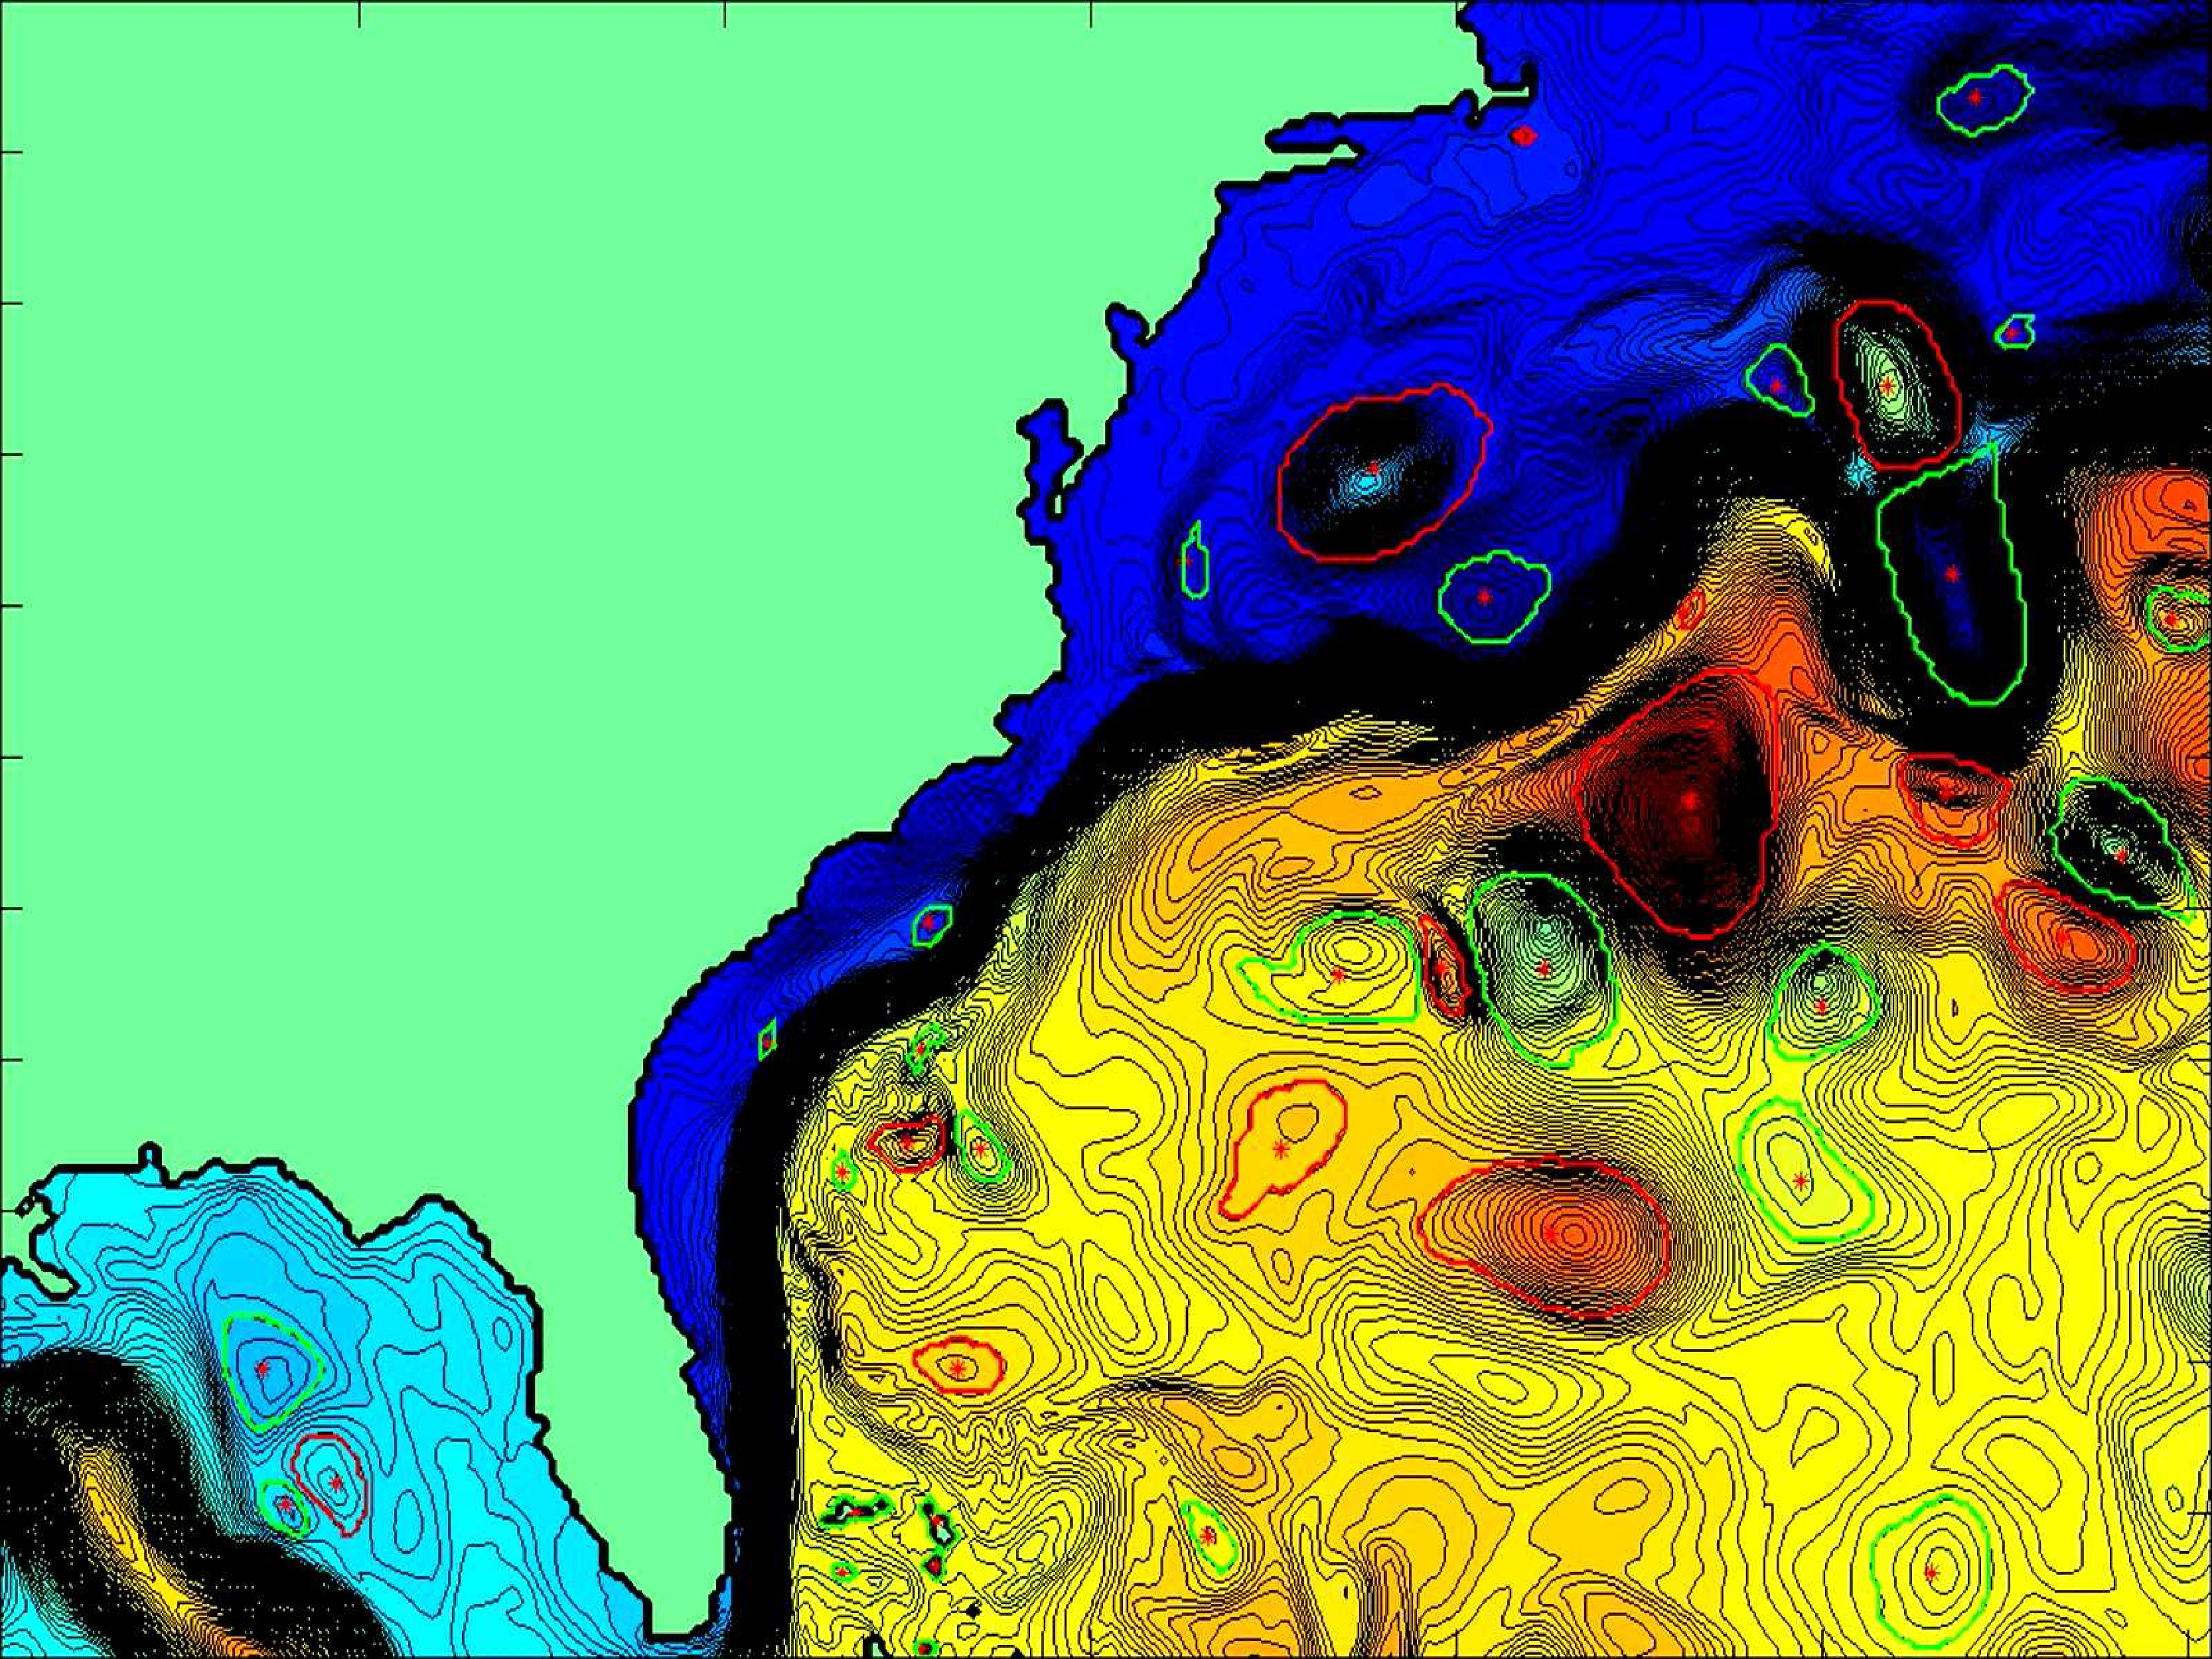
\includegraphics[width=300pt,keepaspectratio=true]{GS.pdf}
	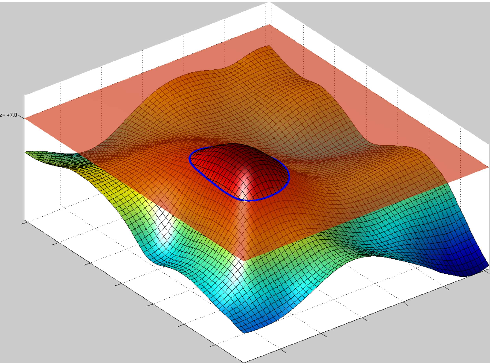
\includegraphics[height=200pt,keepaspectratio=true]{shrunks/slice5.pdf}
\end{figure}
\end{frame}

\begin{frame}
 %\frametitle{Isoperimetric Quotient (IQ): $A/A_{c}=\frac{A}{\pi r_{c}^{2}}=\frac{A}{\pi \left( \frac{c}{2\pi} \right)^{2}}=\frac{4 \pi A}{c}$}
 \frametitle{Isoperimetric Quotient}
  $IQ= A/A_{c}=\frac{4 \pi A}{c}$
\begin{figure}
	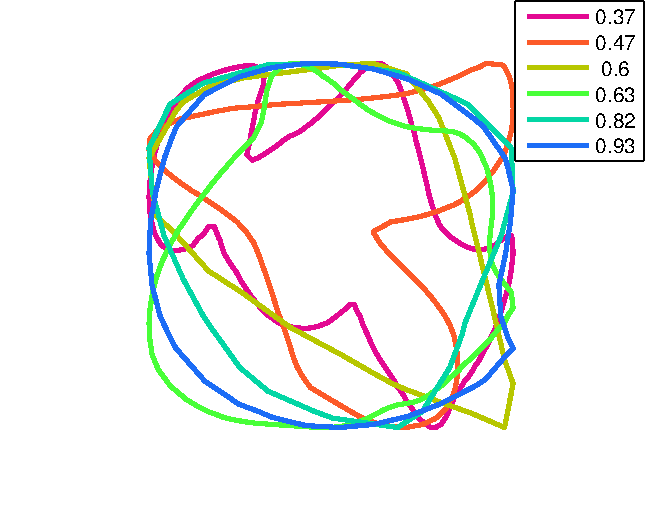
\includegraphics[height=150pt,keepaspectratio=true]{shrunks/isoper.pdf}
\end{figure}
\end{frame}

\begin{frame}
 \frametitle{new problem: deformed eddies get rejected}
\begin{figure}
	\centering
	%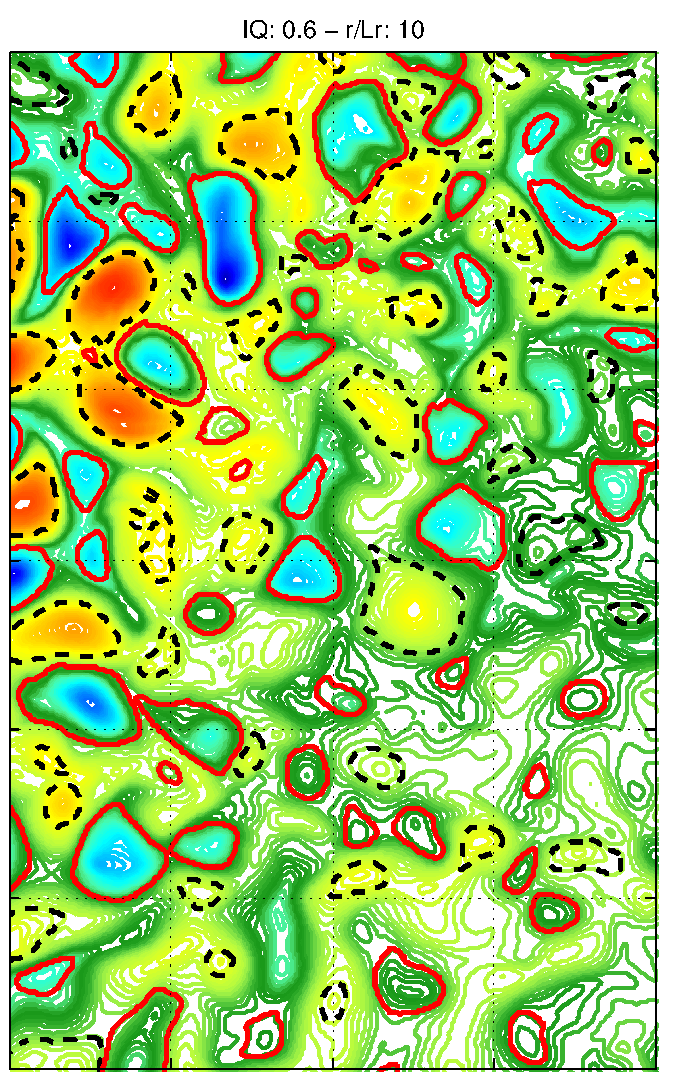
\includegraphics[height=200pt,keepaspectratio=true]{shrunks/iq6dlMrIc.pdf}
	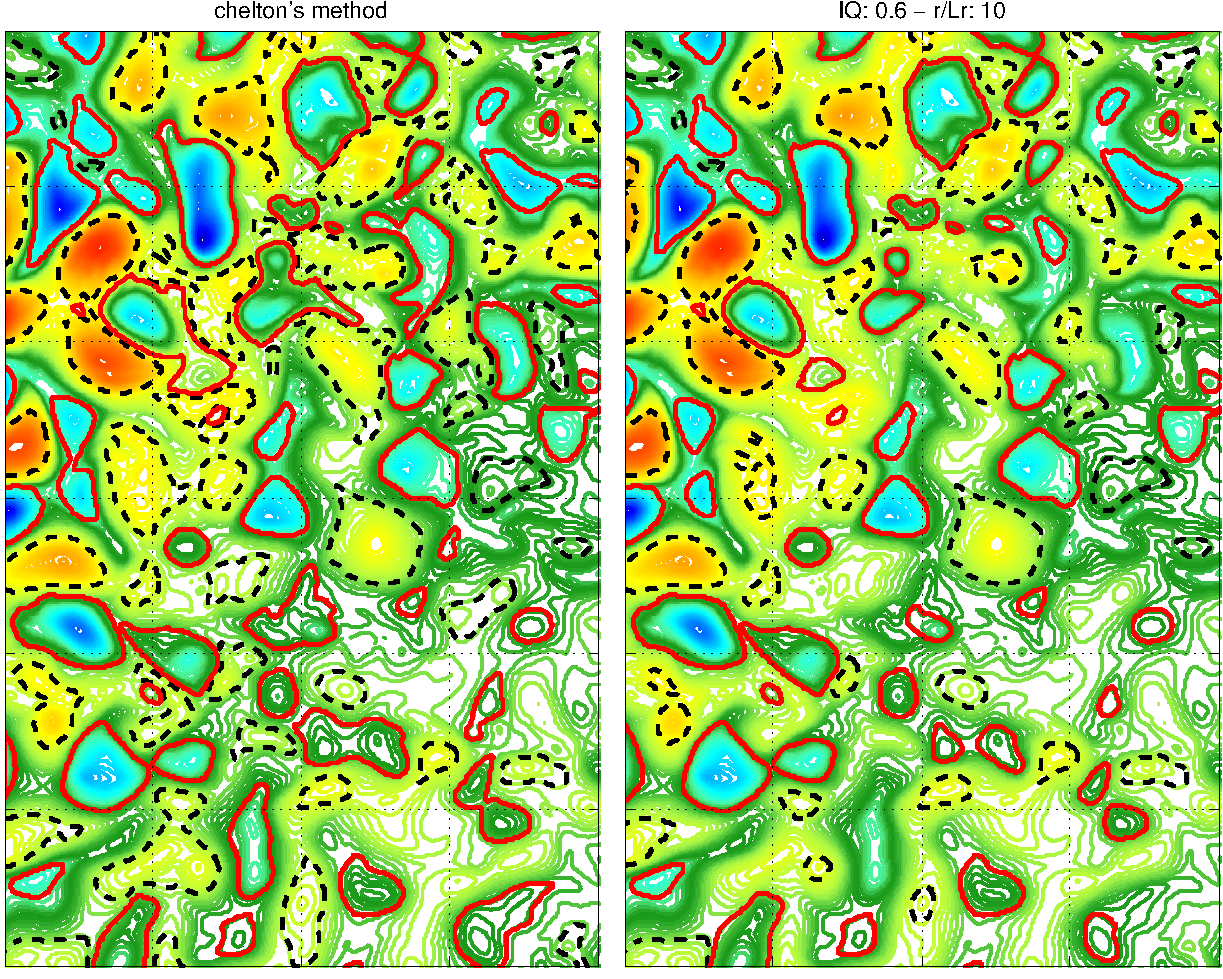
\includegraphics[height=200pt,keepaspectratio=true]{ch2iq6.pdf}
\end{figure}
\end{frame}


\begin{frame}
 \frametitle{solution: allow more deformation but limit hor. scale}
\begin{figure}
	\centering
% 	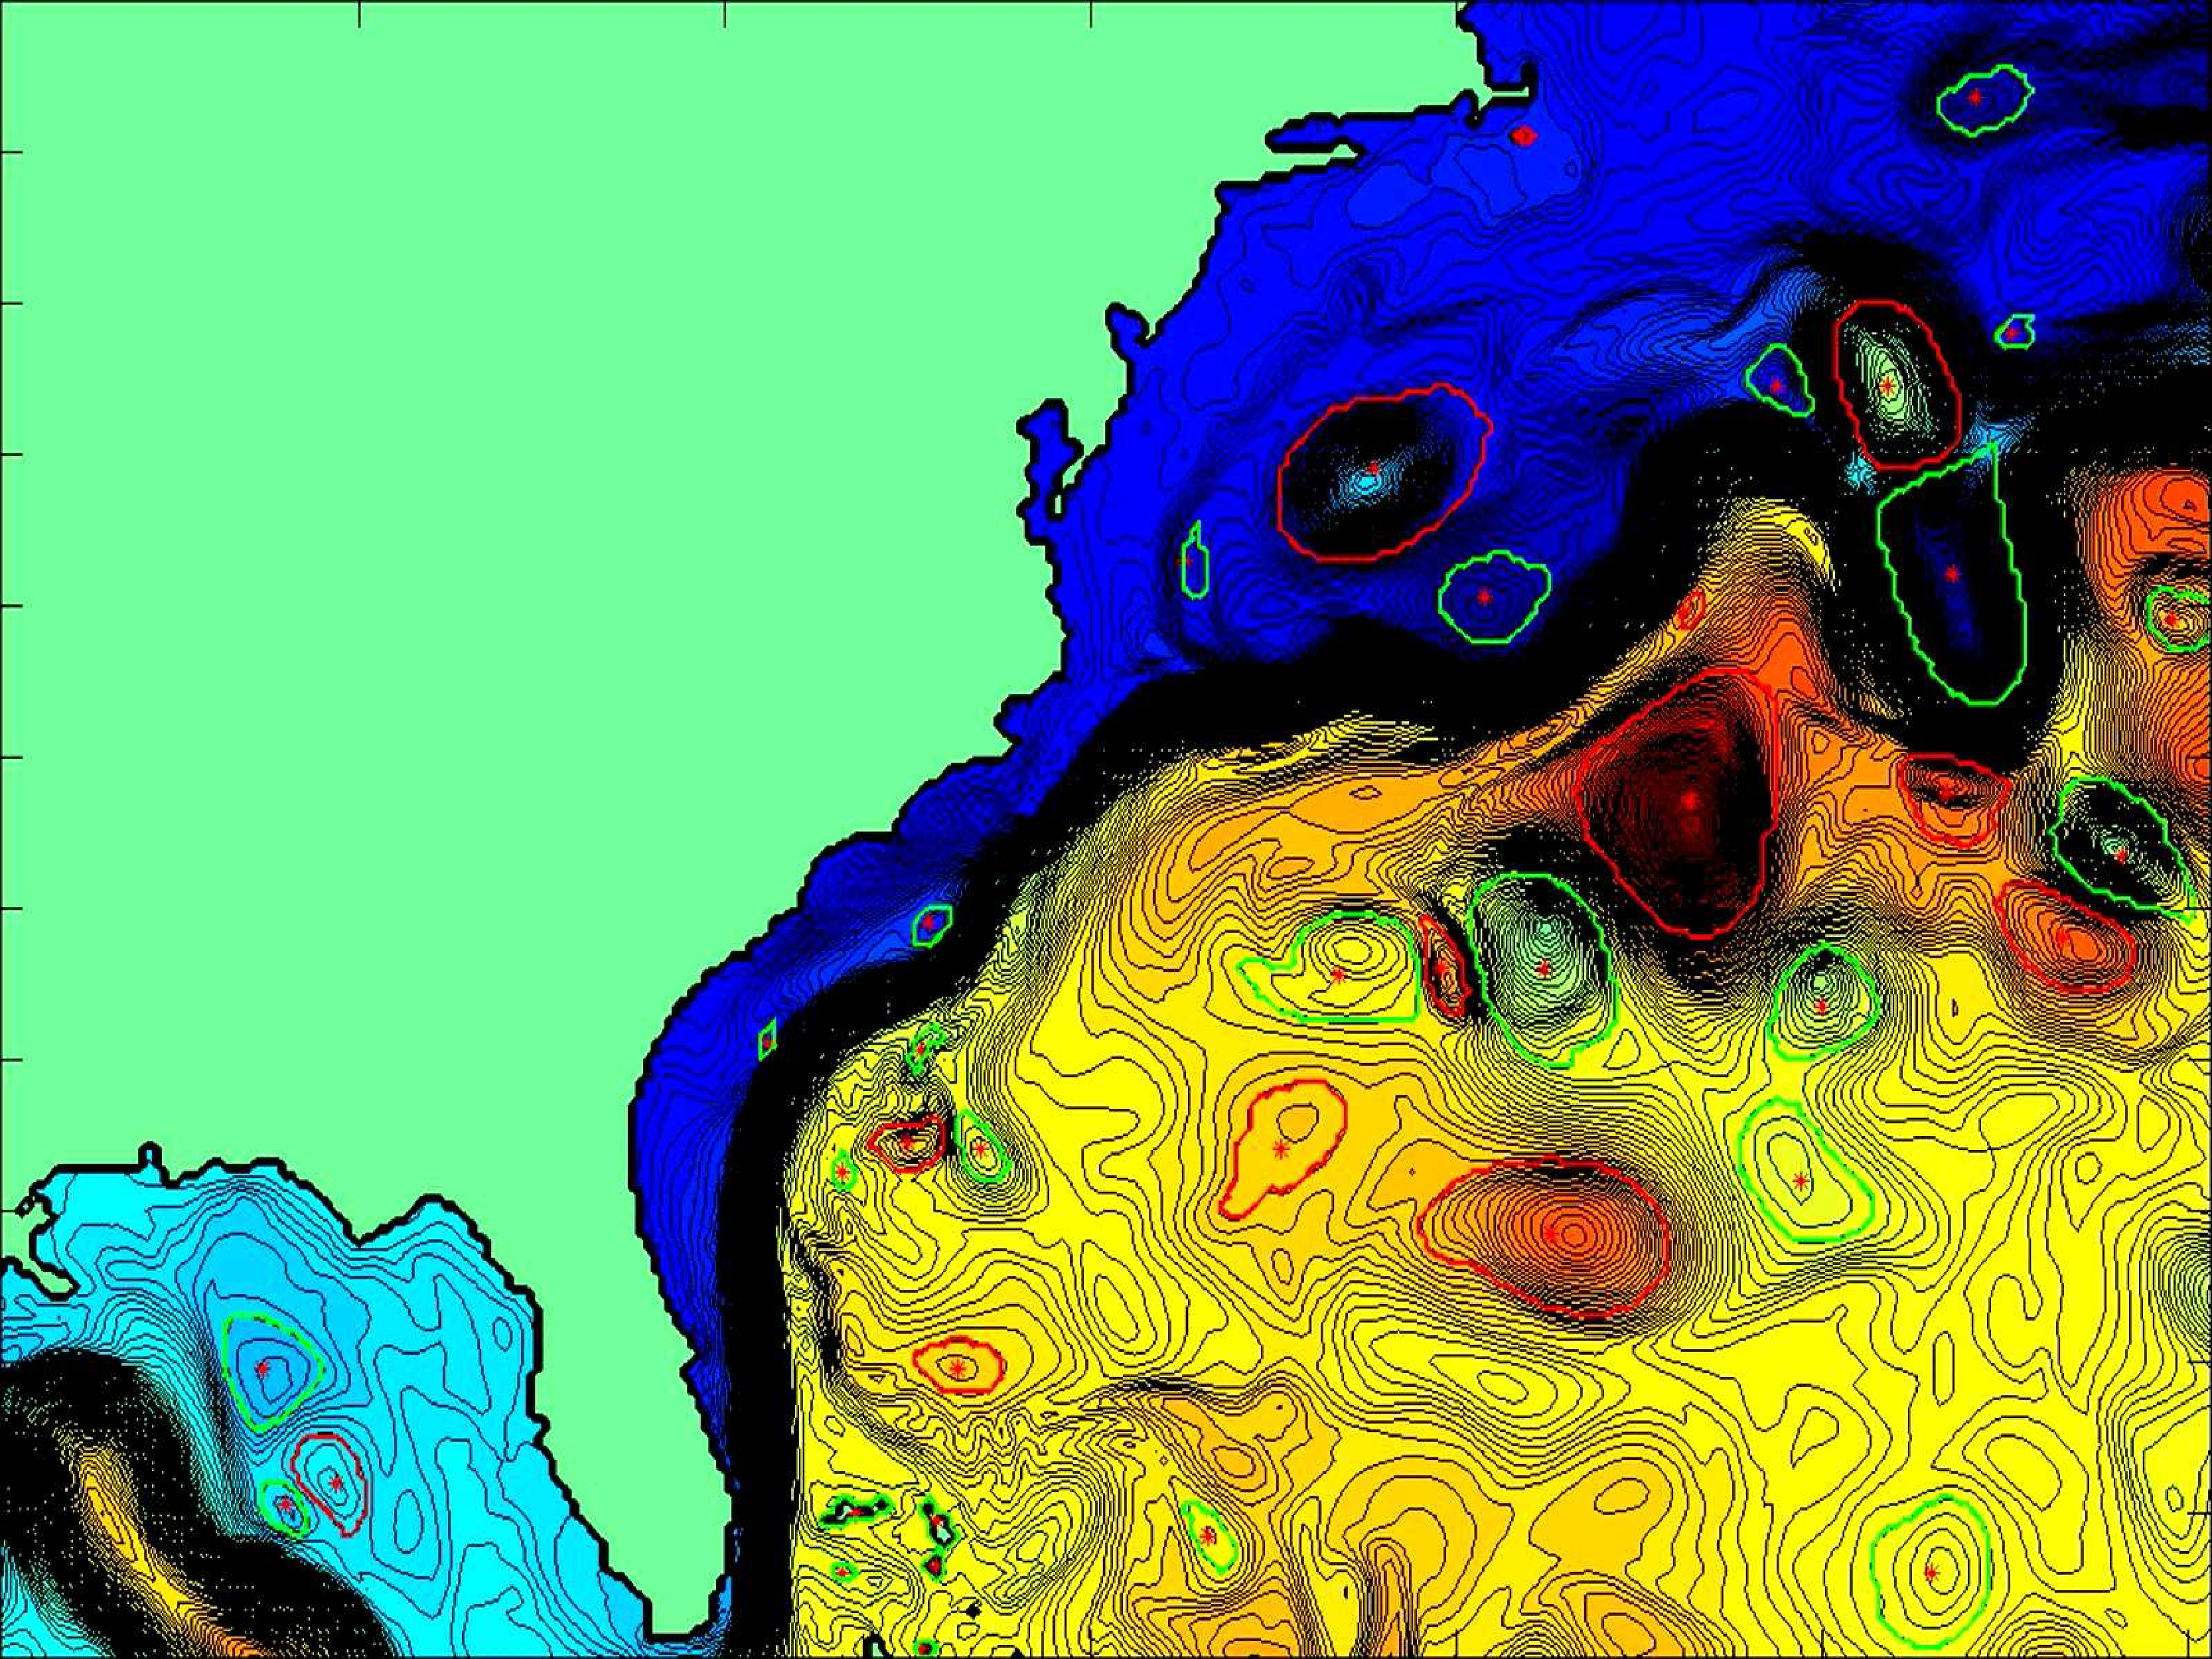
\includegraphics[width=300pt,keepaspectratio=true]{GS.pdf}
	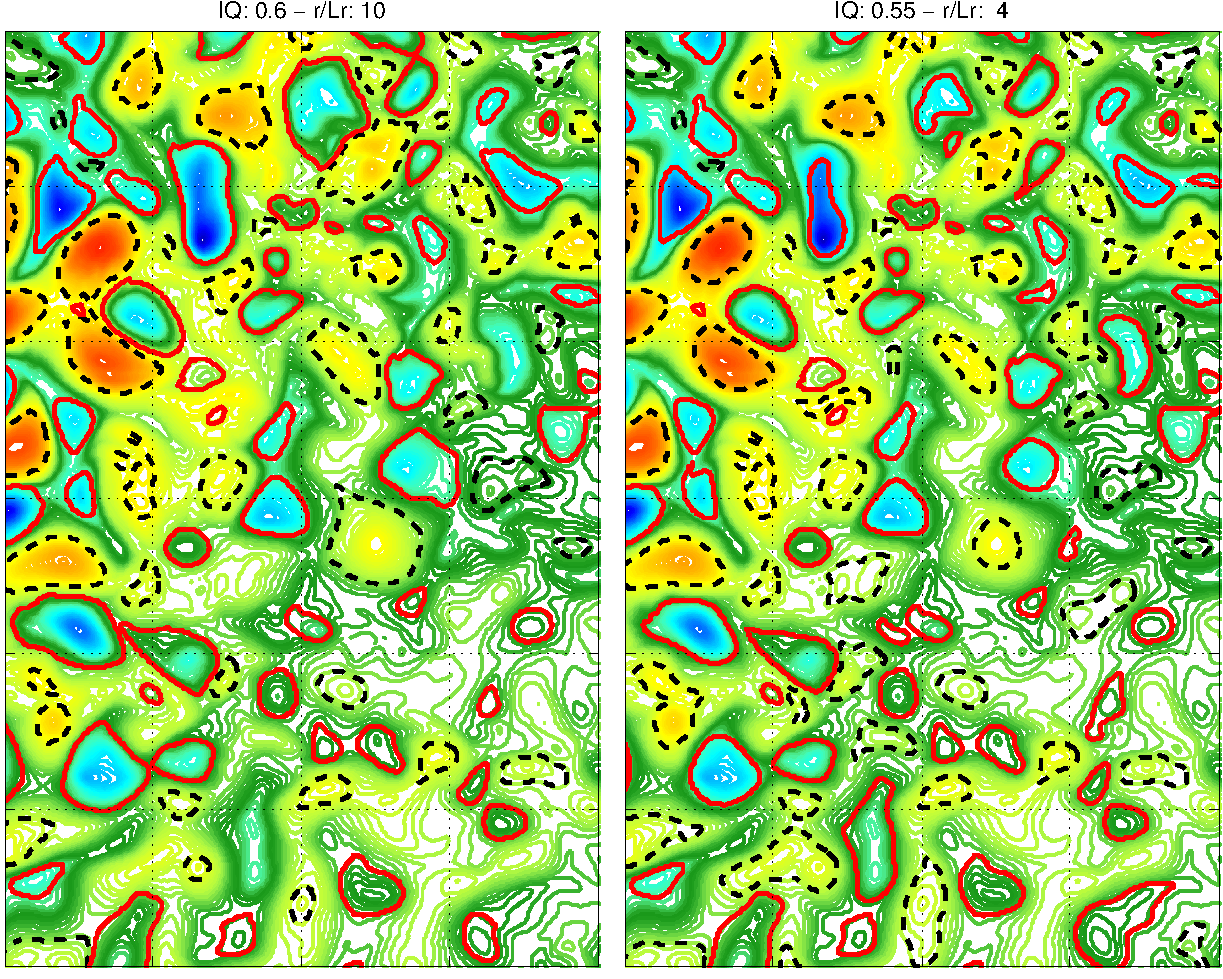
\includegraphics[height=200pt,keepaspectratio=true]{shrunks/iq6toiq55.pdf}
\end{figure}
\end{frame}


%\subsection{Tracking}
%
\begin{frame}
 \frametitle{Tracking}
\begin{enumerate}
\item
Build distance matrix $\vec{D}(old,new)$ between all eddies($t=now-dt$) to all eddies($t=now$).
\item
Flag all $\vec{D}(old,new) > $ threshld.
\item
Flag all not meeting a \textit{similarity criterion} (function of scale and amplitude).
\item
$min(\vec{D})$ in both directions.
\begin{itemize}
\item
agreement: eddy is tracked!\\
$\rightarrow$ append to respective track in running archive.
\item
no new eddy agrees with old eddy: eddy just died..\\
$\rightarrow$ if age $\ge$ threshold, write track to archive, else delete!
\item
no old eddy agrees with new eddy: a new eddy was born\\
$\rightarrow$ initiate new track in running archive.
\end{itemize}
\end{enumerate}
\end{frame}


\begin{frame}[noframenumbering]
 \frametitle{Tracking}
\begin{enumerate}
\item
Build distance matrix $\vec{D}(old,new)$ between all eddies($t=now-dt$) to all eddies($t=now$).
\item
Flag all $\vec{D}(old,new) > $ threshld.
\item
Flag all not meeting a \textbf{\textit{similarity criterion}} (\textbf{function of scale and amplitude}).
\item
$min(\vec{D})$ in both directions.
\begin{itemize}
\item
agreement: eddy is tracked!\\
$\rightarrow$ append to respective track in running archive.
\item
no new eddy agrees with old eddy: eddy just died..\\
$\rightarrow$ if age $\ge$ threshold, write track to archive, else delete!
\item
no old eddy agrees with new eddy: a new eddy was born\\
$\rightarrow$ initiate new track in running archive.
\end{itemize}
\end{enumerate}
\end{frame}


\begin{frame}
\frametitle{What is the scale and amplitude of an eddy ???}
 \begin{figure}
\centering
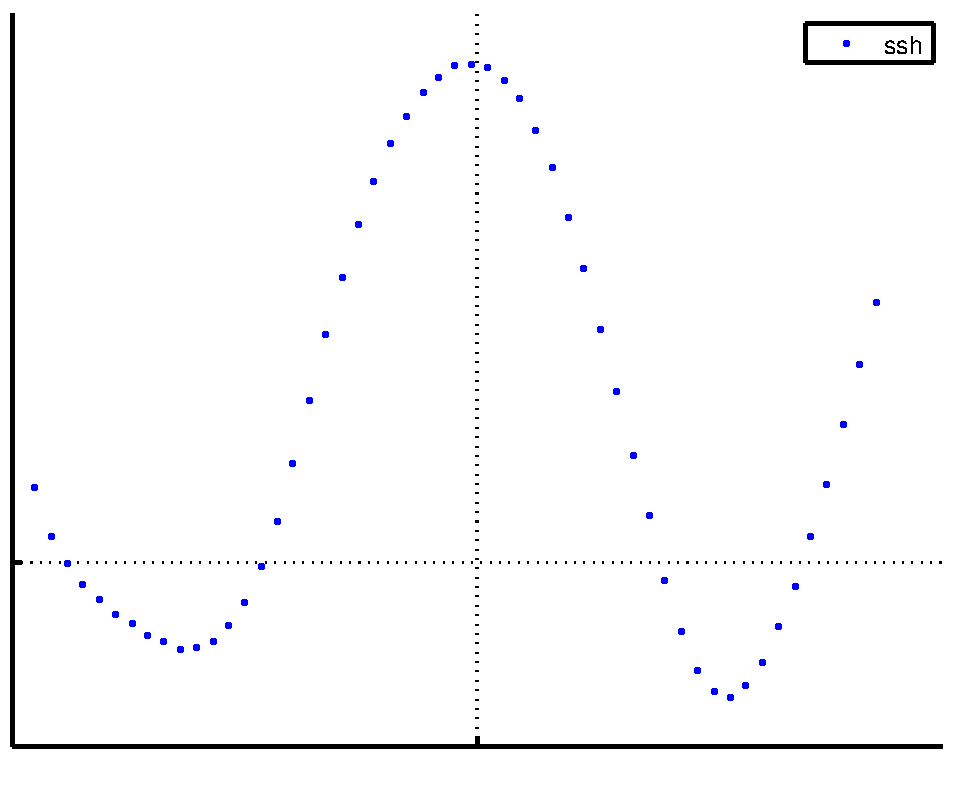
\includegraphics[height=200pt,keepaspectratio=true]{Na.pdf}
\end{figure}
\end{frame}


\begin{frame}
 \frametitle{example: meander}
\begin{figure}
\centering
	%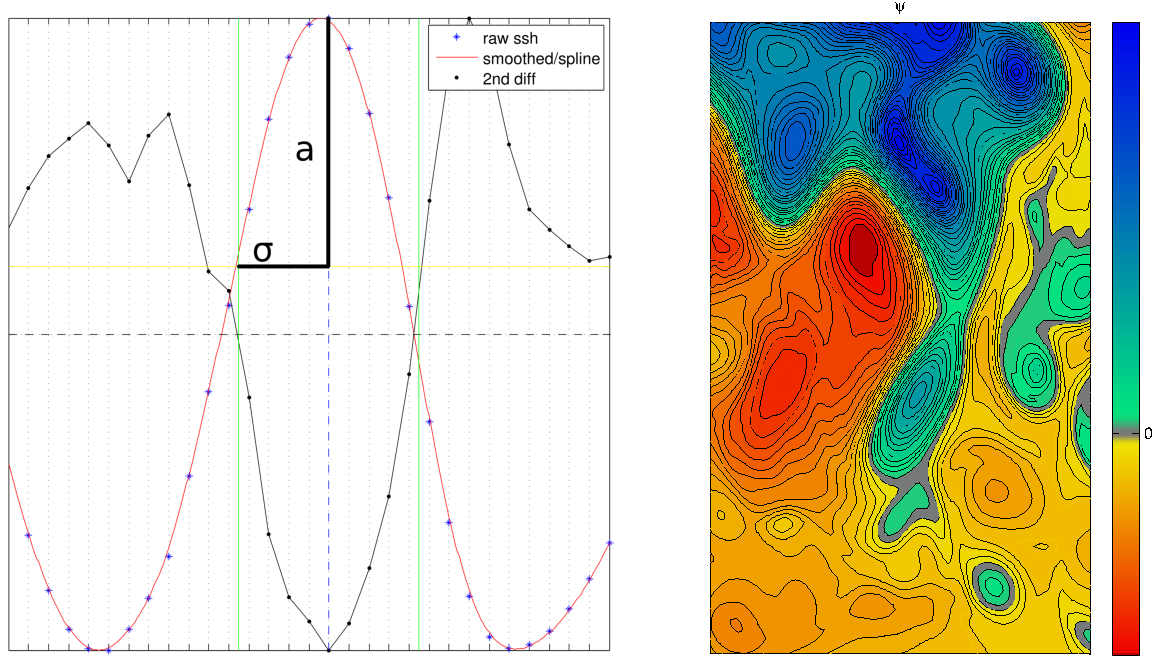
\includegraphics[width=300pt,keepaspectratio=true]{prof3bPsi.pdf}
	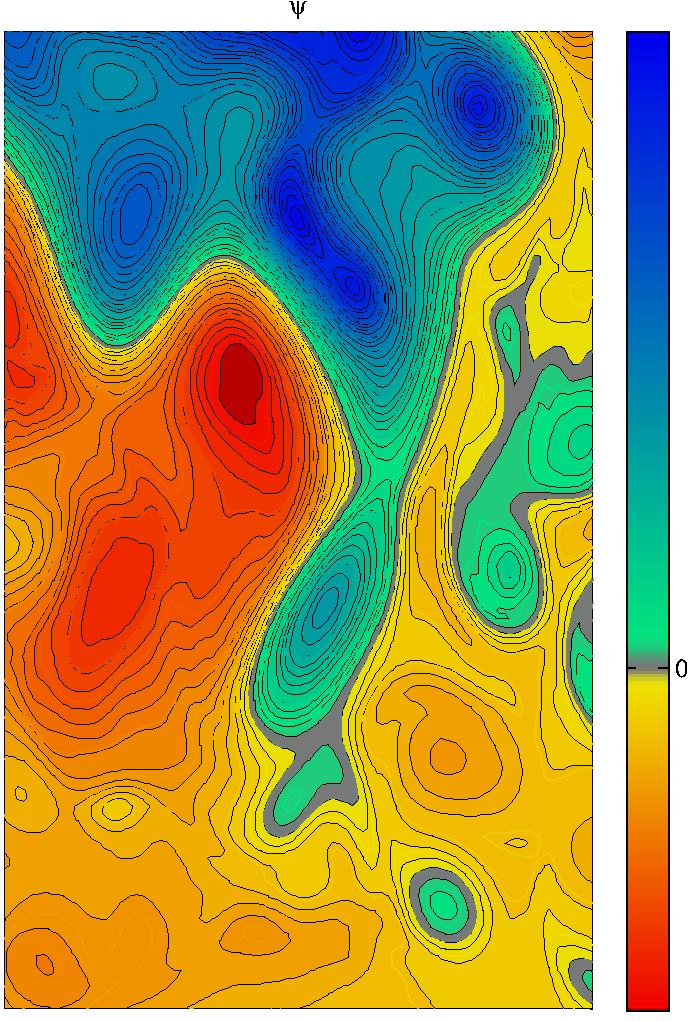
\includegraphics[height=200pt,keepaspectratio=true]{psi.pdf}
\end{figure}
\end{frame}


\begin{frame}
\frametitle{Problem: coarse resolution}
$ \partial_x \sim \vec{U}, \; \partial_{xx} \sim \vec{\omega}$
 \begin{figure}
\centering
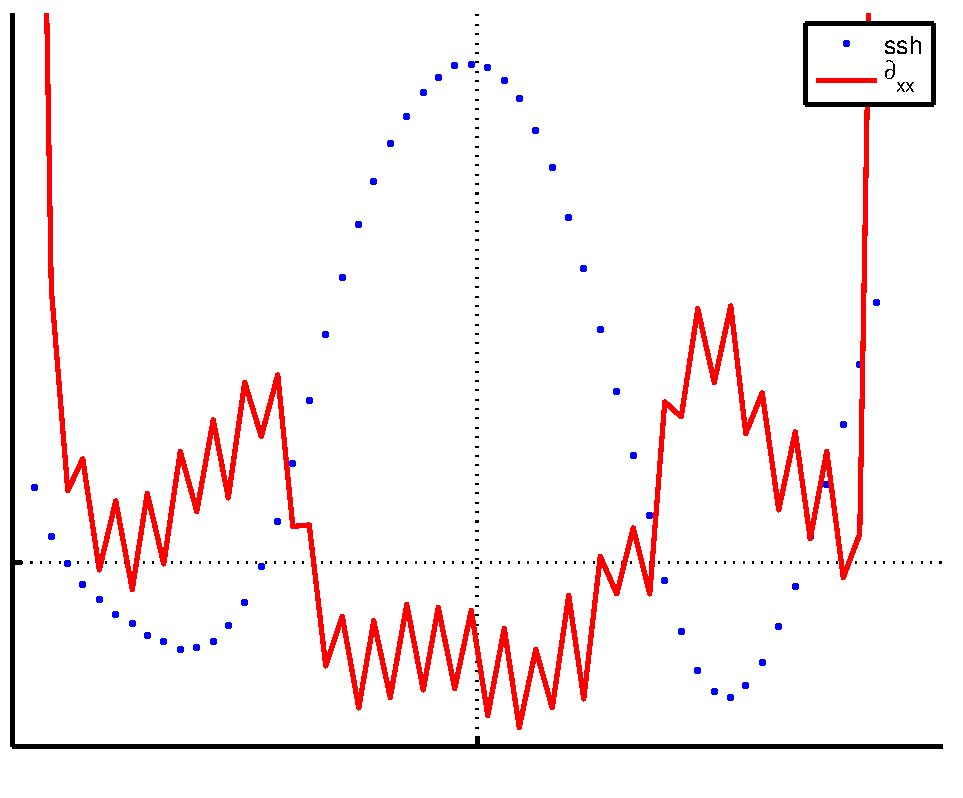
\includegraphics[height=200pt,keepaspectratio=true]{Nb.pdf}
\end{figure}
\end{frame}


\begin{frame}
\frametitle{Solution: Interpolate and use Fourier Series for differentials}
 \begin{figure}
\centering
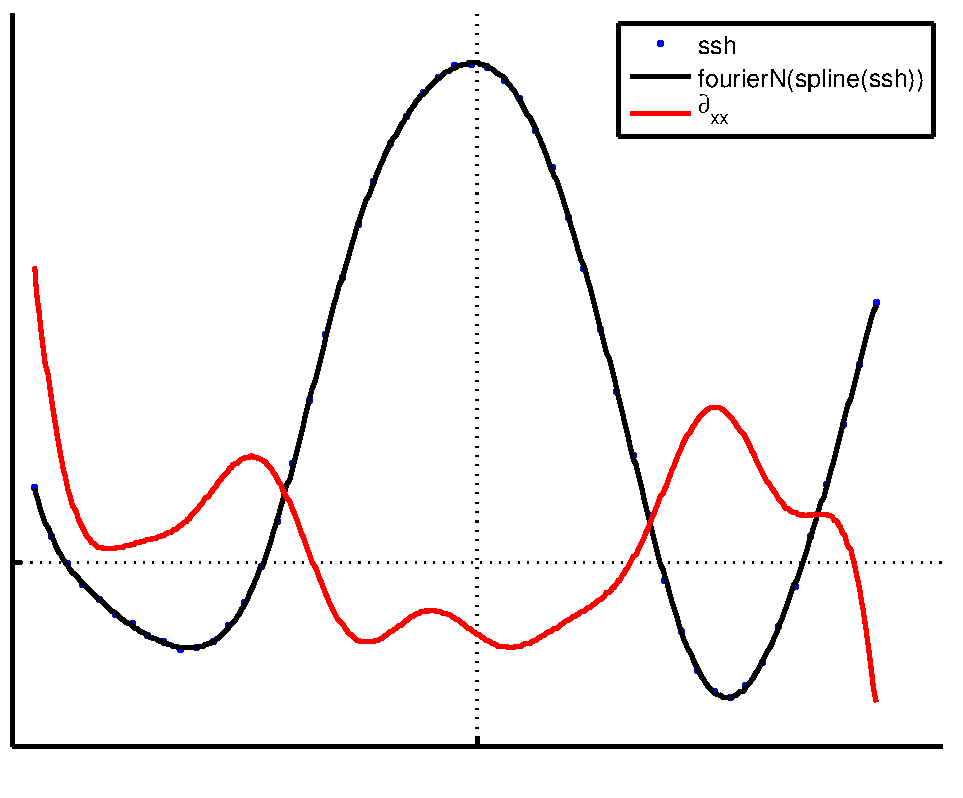
\includegraphics[height=200pt,keepaspectratio=true]{Nc.pdf}
\end{figure}
\end{frame}

\begin{frame}
\frametitle{Assuming gauss shape:  $A \exp{\left(- x^2/2\sigma^2\right)}; \;\;a=A(1-\exp{-1/2})$}
All shape-defining parameters for the \textit{similarity criterion} are determined!  
 \begin{figure}
\centering
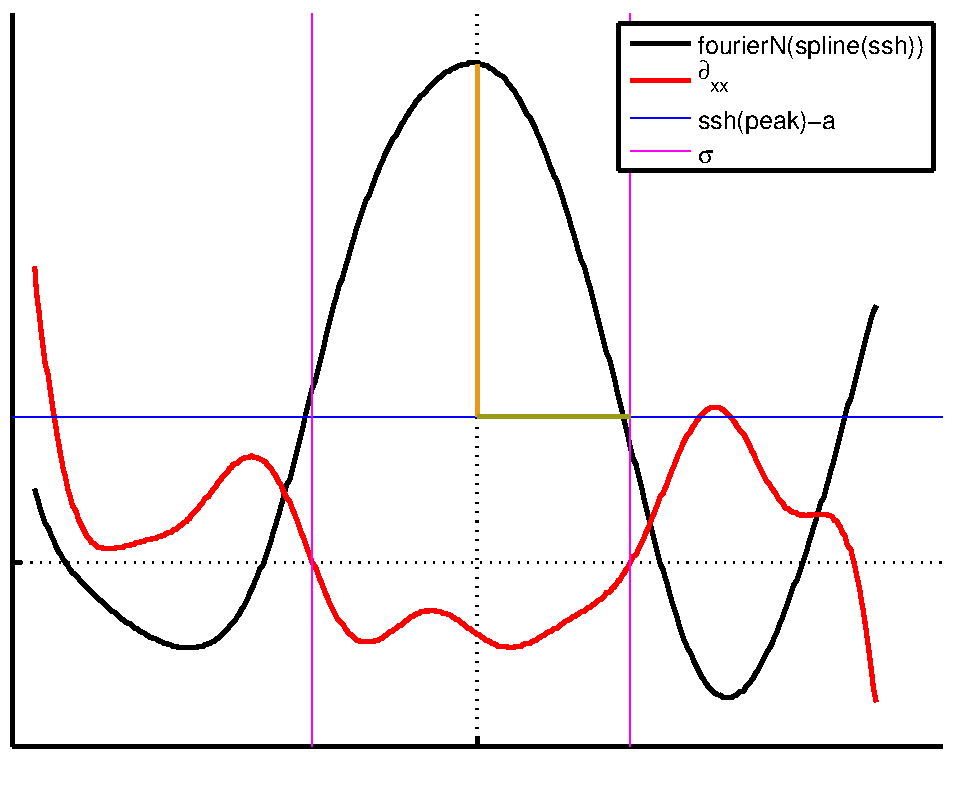
\includegraphics[height=200pt,keepaspectratio=true]{Ne.pdf}
\end{figure}
\end{frame}


\begin{frame}
\frametitle{Note: Gauss shape assumption not necessary for this method.}
 \begin{figure}
\centering
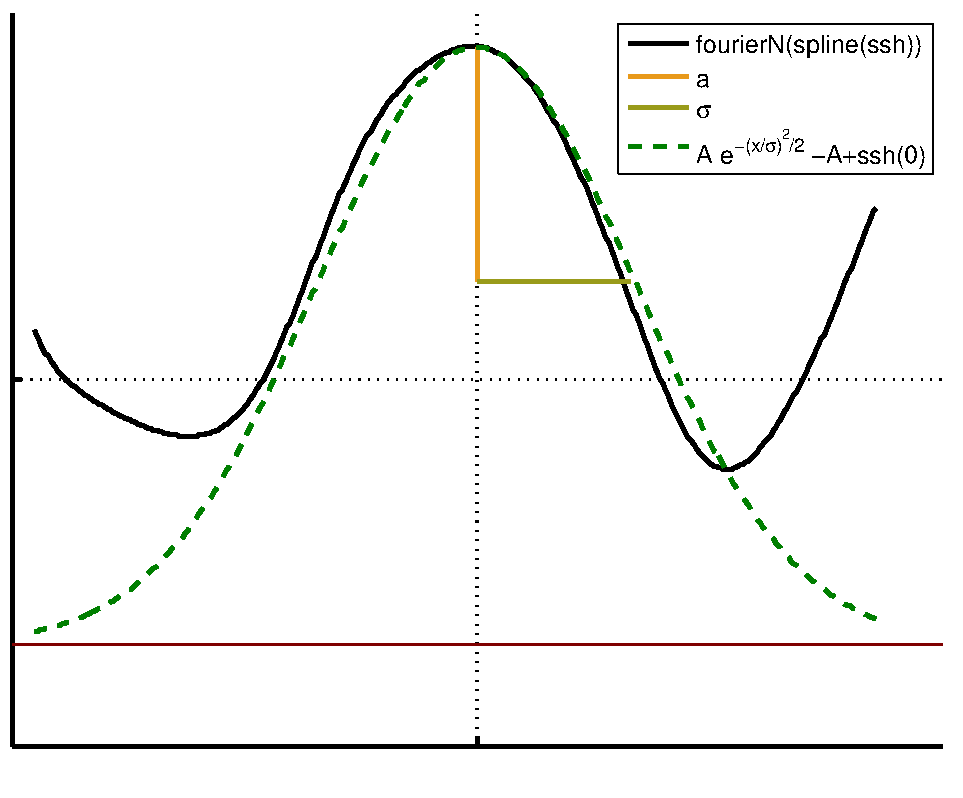
\includegraphics[height=200pt,keepaspectratio=true]{Nf.pdf}
\end{figure}
\end{frame}

\begin{frame}
\frametitle{Chelton et al. define 4 different eddy scales.}
 \begin{figure}
\centering
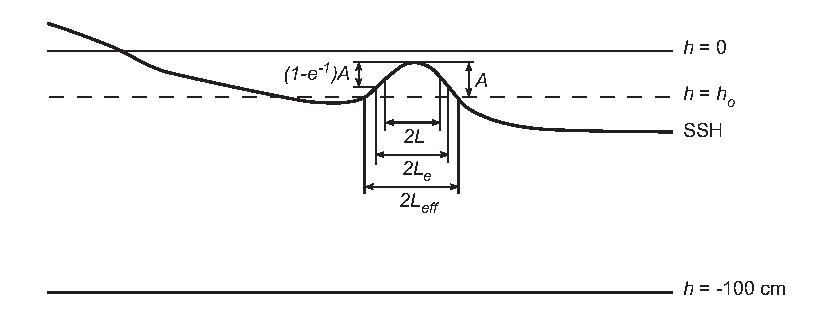
\includegraphics[width=330pt,keepaspectratio=true]{chEs.pdf}
\end{figure}
\end{frame}

\begin{frame}
\frametitle{problematic: broad flat \textit{wobbly} eddies}
 \begin{figure}
\centering
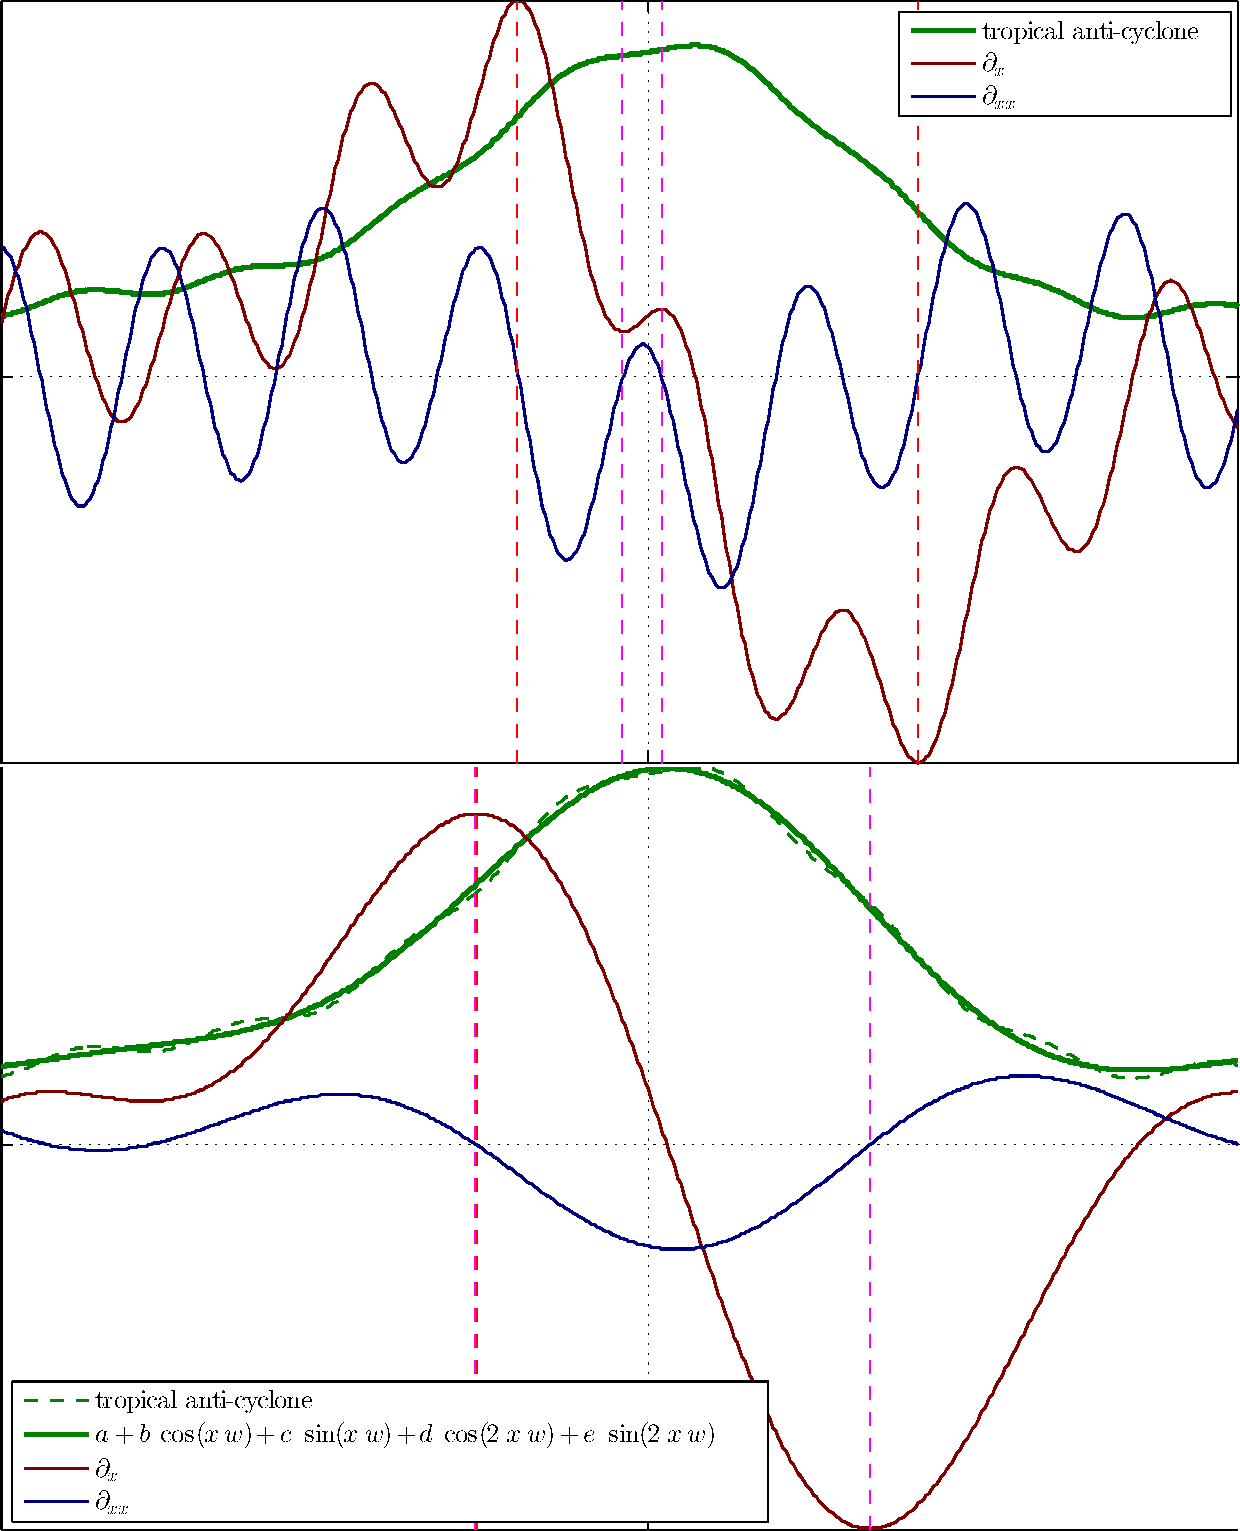
\includegraphics[height=200pt,keepaspectratio=true]{tropicalJmd.pdf}
\end{figure}
\end{frame}

\begin{frame}
	\frametitle{Okubo-Weiss}
	\centering
	\begin{minipage}[T]{1\textwidth}
	\begin{figure}
		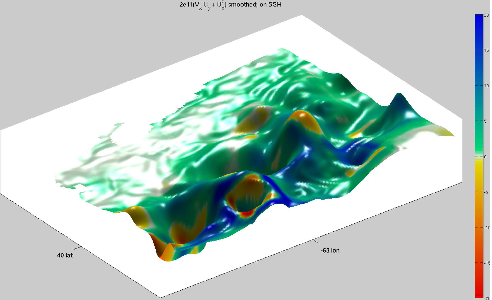
\includegraphics[width=200pt,keepaspectratio=true]{OWpatch2.pdf}
	\end{figure}		
	\end{minipage}
\vfill
	\begin{minipage}[T]{1\textwidth}
		use eigenvalues of 2d deformation tensor to detect vortex: 
		%\begin{align*}
			%%det(\lambda\vec{I} \vec{\Lambda} - \vec{T})=0
			%%&=
			%%(\lambda-u_{x})(\lambda+u_{x}) - v_{x}u_{y} \\
			%%%&=
			%%%\lambda^{2}-u_{x}^{2} - v_{x}u_{y}\\ 
			%\lambda
			%&=
			%\pm \sqrt{u_{x}^{2} + v_{x}u_{y}}
		%\end{align*}
\begin{align*}
& det(\lambda\vec{I}- \vec{\grad \vec{u}}) =0\\
&\lambda^{2} =OW/2=2 u_{x}^{2} + v_{x}u_{y}
\end{align*}	
%\begin{align*}
%& det(\lambda\vec{I}- \vec{\grad \vec{u}}) =0\\
%&\lambda^{2} =OW/2=\tikzmarkin[fill=yellow]{first eq}u_{x}^{2} + v_{x}u_{y}\tikzmarkend{first eq} 
%%&=-(\vort{u})^{2} + (\div{\vec{u}})^{2} + (\grad_{\updownarrow} \cdot \vec{u})^{2}	+ (\underaccent{90^{\circ}}{\grad} \cdot\vec{u})^{2}	\\	&=-vorticity^{2}+divergence^{2}+shear^{2}+stretching^{2}\\& = OW/4
%\end{align*}		
\end{minipage}
\end{frame}


\begin{frame}
\frametitle{Removing larger scale signals important for Chelton's method.}
\begin{figure}
	\centering
	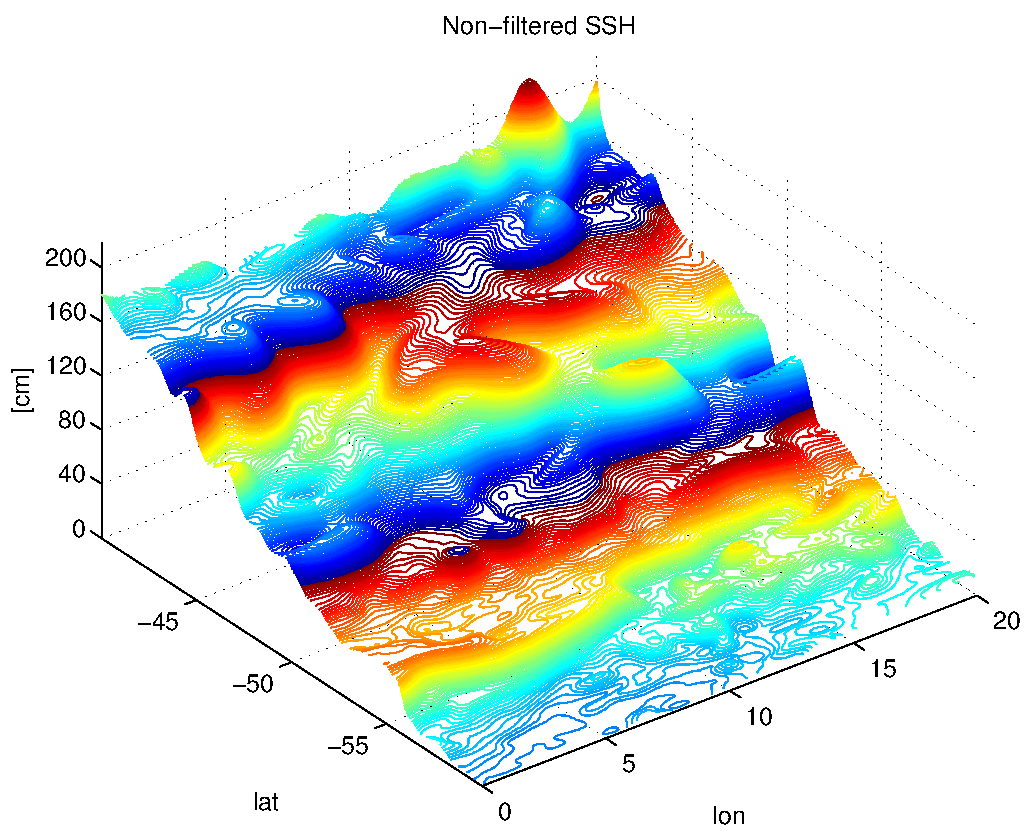
\includegraphics[height=200pt,keepaspectratio=true]{shrunks/Non-filtered_SSH.pdf}
\end{figure}
\end{frame}

\begin{frame}[noframenumbering]
\frametitle{easiest: subtract annual mean}
\begin{figure}
	\centering
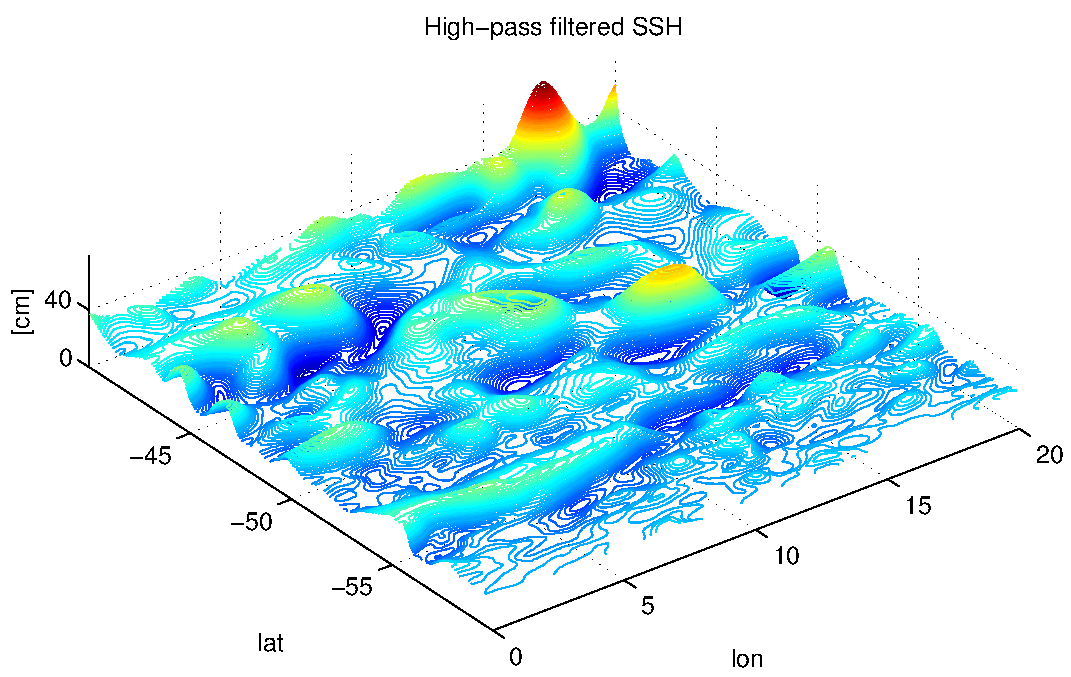
\includegraphics[width=300pt,keepaspectratio=true]{shrunks/High-pass_filtered_SSH.pdf}
\end{figure}
\end{frame}





\begin{frame}
\frametitle{finding a suitable scale threshold}
\begin{figure}
	\centering
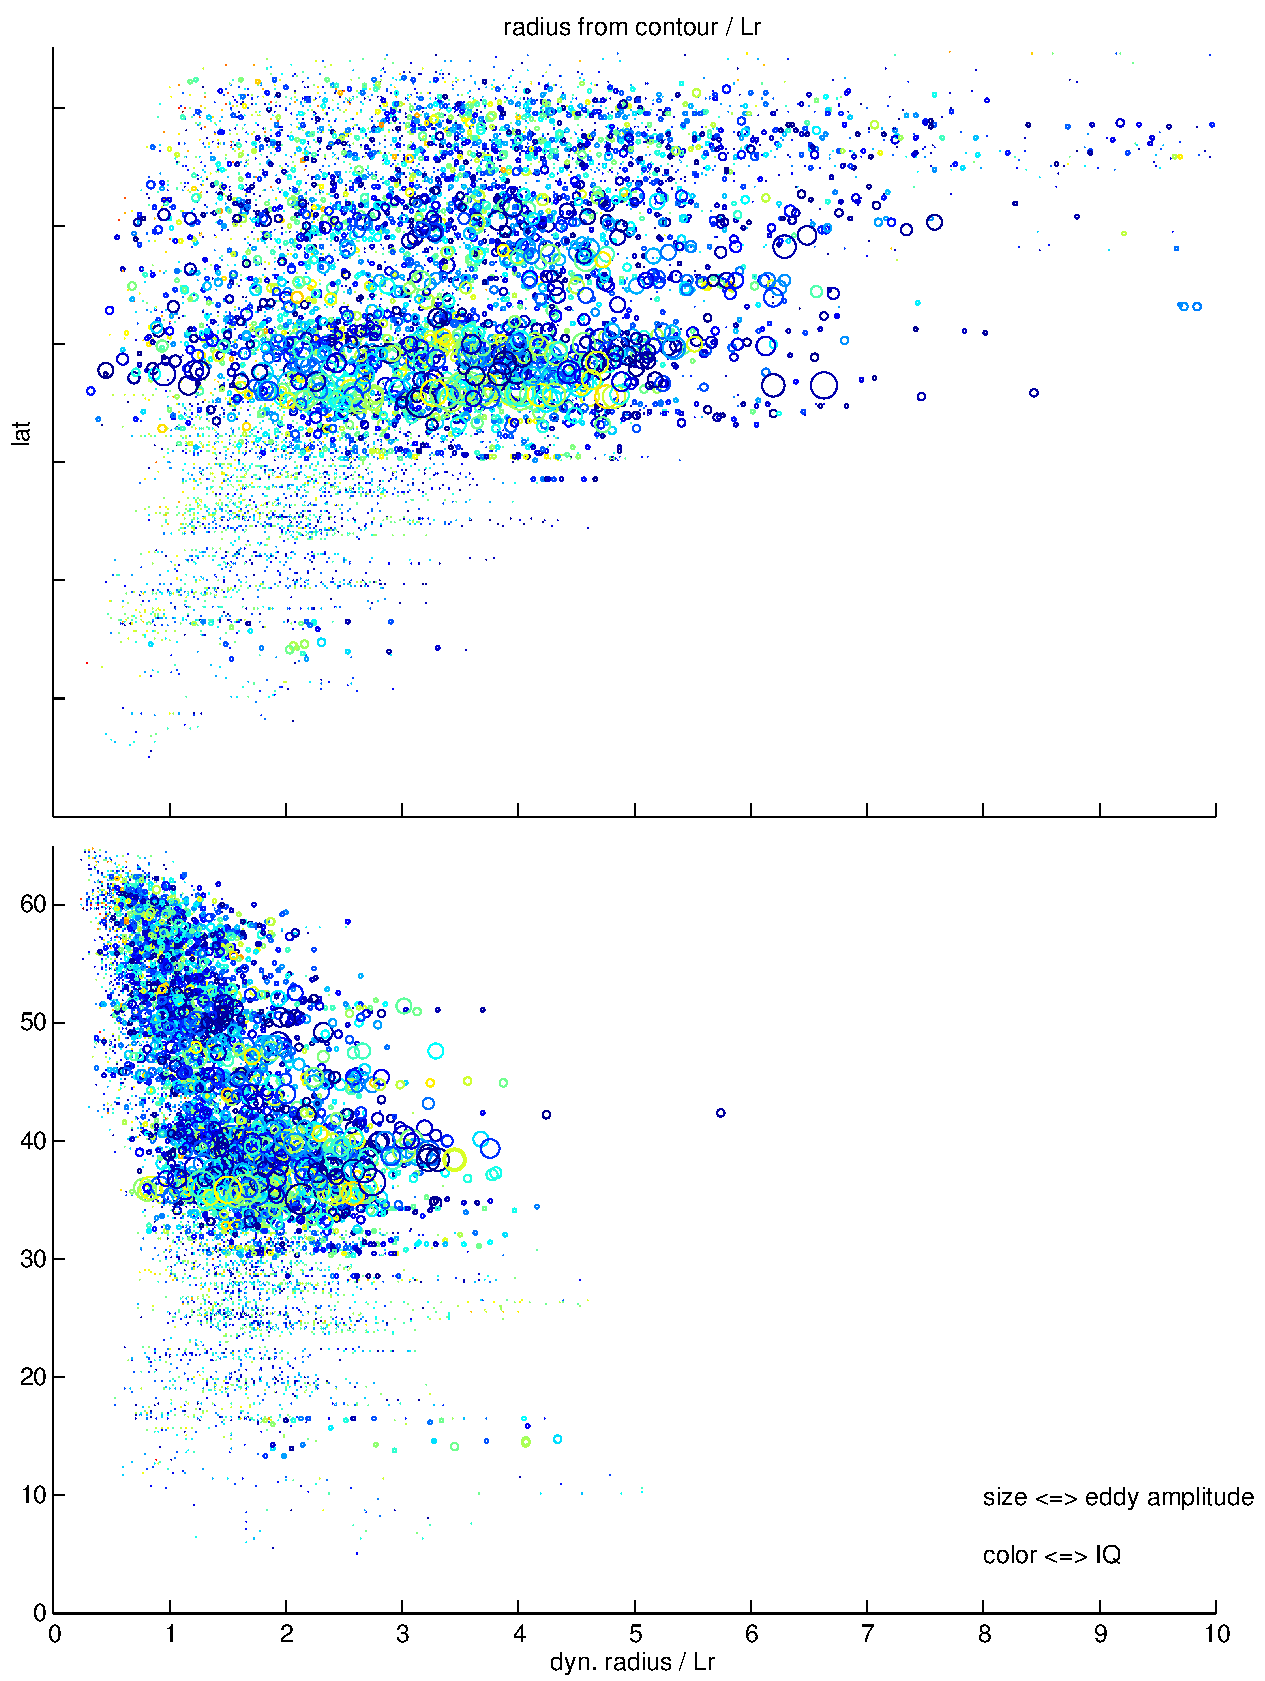
\includegraphics[height=240pt,keepaspectratio=true]{shrunks/scatRadOLrComp.pdf}
\end{figure}
\end{frame}

\begin{frame}[noframenumbering]
\begin{figure}
	\centering
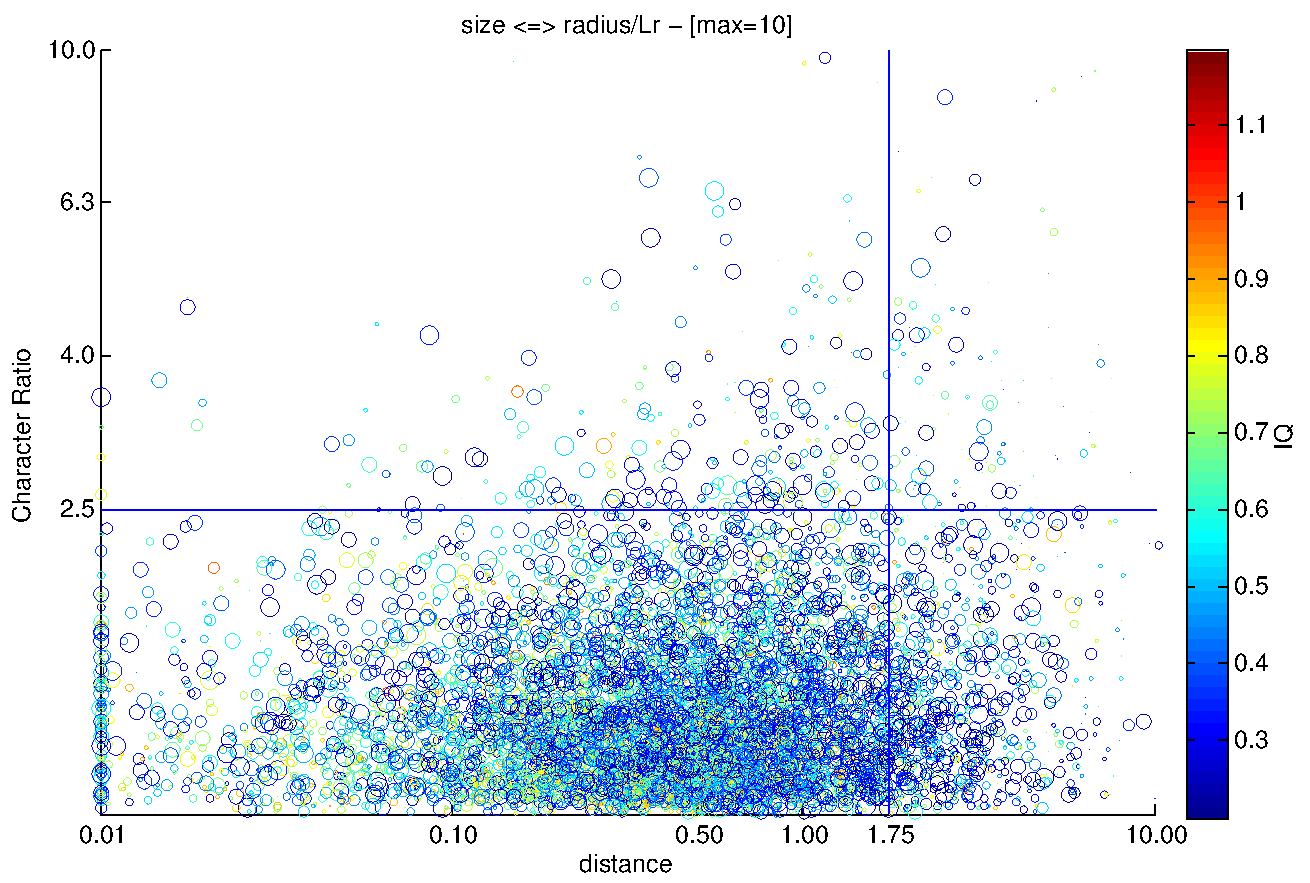
\includegraphics[width=300pt,keepaspectratio=true]{shrunks/scat1.pdf}
\end{figure}
\end{frame}

\begin{frame}[noframenumbering]
\begin{figure}
	\centering
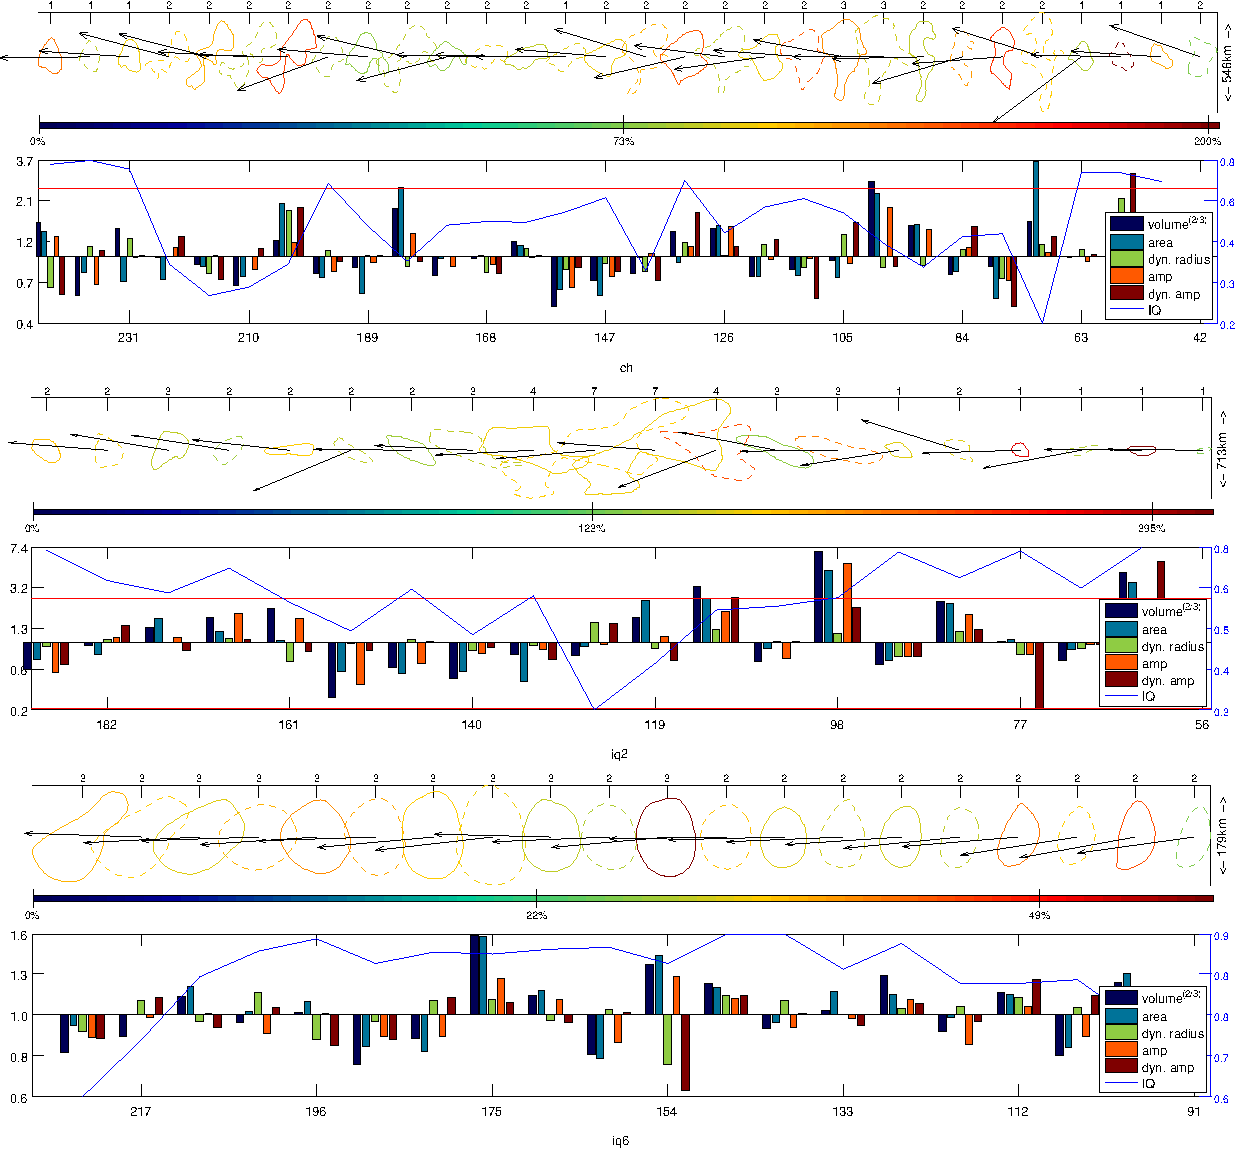
\includegraphics[height=260pt,keepaspectratio=true]{parAnalAll.pdf}
\end{figure}
\end{frame}


\begin{frame}[noframenumbering]
\begin{figure}
	\centering
	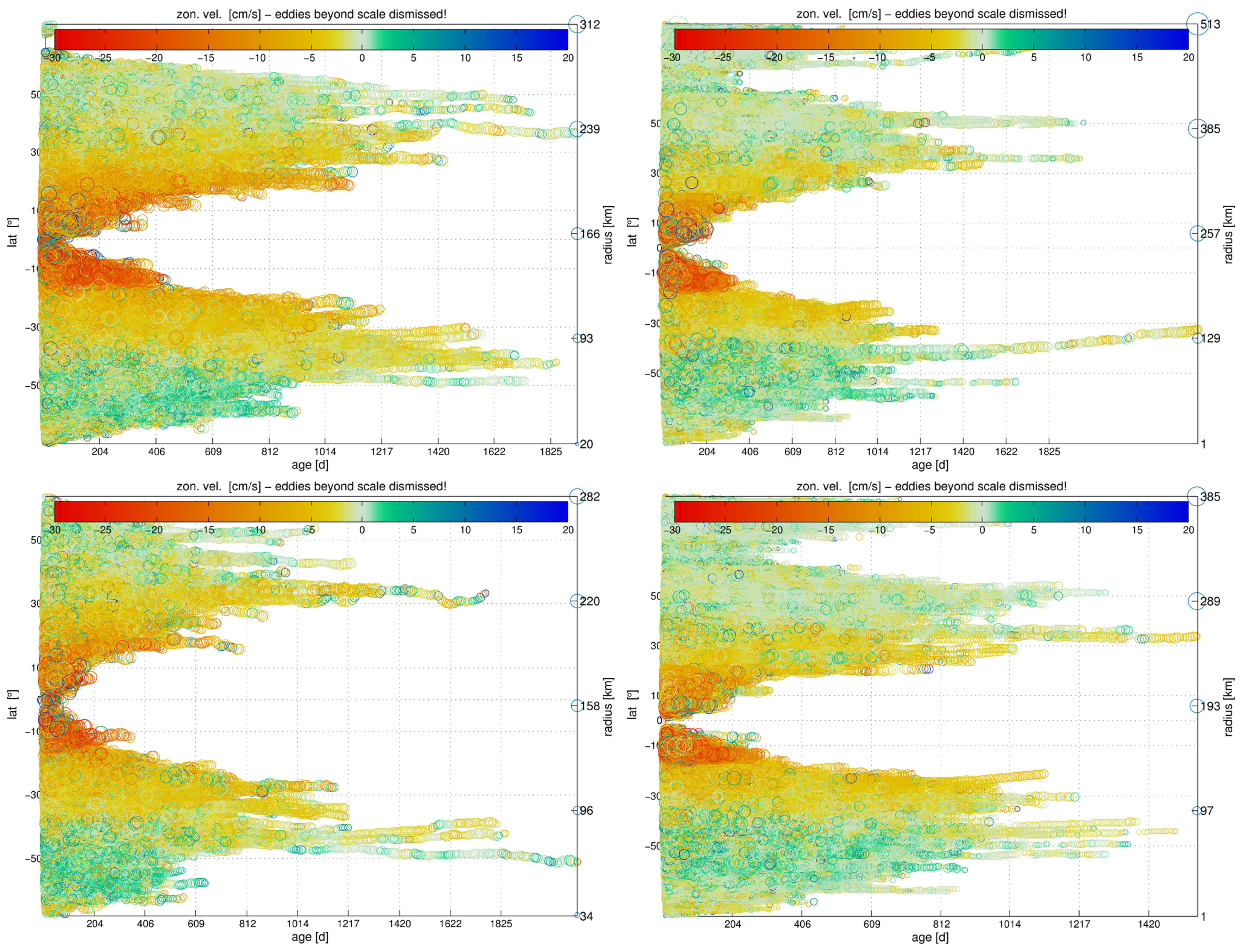
\includegraphics[width=300pt,keepaspectratio=true]{SCTall.pdf}
\end{figure}
\end{frame}


%% appendix



%\begin{frame}
%\frametitle{assume gauss shape:  $A \exp{\left(- x^2/2\sigma^2\right)}$}
 %\begin{figure}
%\centering
%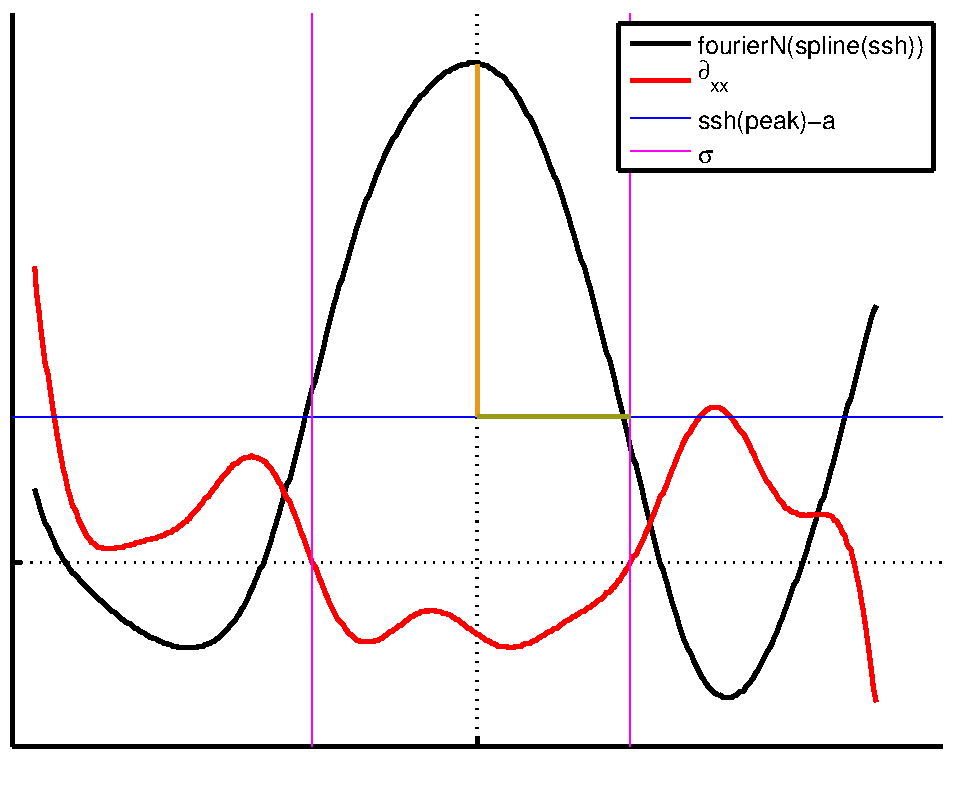
\includegraphics[height=200pt,keepaspectratio=true]{Ne.pdf}
%\end{figure}
%\end{frame}



%\begin{frame}	
%\begin{align*}
	%\left| \lambda \vec{I} - \grad \vec{u} \right|
	%&=
%\begin{vmatrix}
 %\lambda - u_{x} & u_{y} \\
 %v_{x} & \lambda - v_{y}
 %\end{vmatrix}	\\
 %&=
 %\left(  	\lambda - u_{x} \right)  \left( 	\lambda - v_{y} \right){}
 %- v_{x} u_{y}\\
 %\lambda^{2}&=
 	  %u_{x}^{2}
 %+ v_{x} u_{y}
%\end{align*}

%\begin{align*}
	%\left| \lambda \vec{I} - \vec{\Omega}  \right|
	%&=
%\frac{1}{2}\begin{vmatrix}
 %\lambda & u_{y}-v_{x} \\
 %-u_{y}+v_{x} & \lambda 
 %\end{vmatrix}	\\
 %2\lambda_{\Omega}^{2}
 %&=
 %u_{y}^{2}-2u_{y}v_{x}+v_{x}^{2}
%\end{align*}

%\begin{align*}
	%\left| \lambda \vec{I} - \vec{E}  \right|
	%&=
%\frac{1}{2}\begin{vmatrix}
 %\lambda -2u_{x} & u_{y}+v_{x} \\
 %u_{y}+v_{x} & \lambda -2v_{y}
 %\end{vmatrix}	\\
 %%&(\lambda -2u_{x} ) (\lambda +2u_{x})
 %%-u_{y}^{2}-2u_{y}v_{x}-v_{x}^{2}  
 %%\\
  %2\lambda_{E}^{2}
 %&=4u_{x}^{2}
 %+u_{y}^{2}
 %+ 2u_{y}v_{x}
 %+v_{x}^{2}  
%\end{align*}
%\begin{align*}
	%-\lambda_{\Omega}^{2} + \lambda_{E}^{2}
	%&=
	 %2u_{y}v_{x}
	 %+2u_{x}^{2}
%\end{align*}



%\end{frame}



%\begin{frame}
%\begin{align*}
%&=-(v_{x}-u_{y})^{2}
%+(u_{x}+v_{y})^{2}
%+(v_{x}+u_{y})^{2}
%+(u_{x}-v_{y})^{2}\\
%&=
%-(
%v_{x}^{2}
%-2v_{x}u_{y}
%+u_{y}^{2}
%)
%+0+
%(
%v_{x}^{2}
%+2v_{x}u_{y}
%+u_{y}^{2}
%)
%+(
%u_{x}^{2}
%-2u_{x}v_{y}
%+v_{y}^{2}
%)\\
%&=
%4v_{x}u_{y}
%+(
%u_{x}^{2}
%-2u_{x}v_{y}
%+v_{y}^{2}
%)\\
%&=
%4v_{x}u_{y}
%+
%4u_{x}^{2}
%\\
%\end{align*} 
%\end{frame}











%\section{New Results}
%\newenvironment{mtrx}[1]
{\begin{tiny}
 \begin{center}
	\hspace{-40pt}
	\vspace{-10pt}
 \begin{tabular}{r|c|c|}
	\multicolumn{1}{c}{} & \multicolumn{1}{c}{aviso} & \multicolumn{1}{c}{pop} \\
	\cline{2-3}
	me & #1  & #1  \\
	\cline{2-3}
	chelton  & #1 & #1  \\
	\cline{2-3}
\end{tabular}
 \end{center}
\end{tiny}
}


\begin{spacing}{.5}

\begin{frame}
	\mtrx{U}
	\begin{figure}
	\centering
	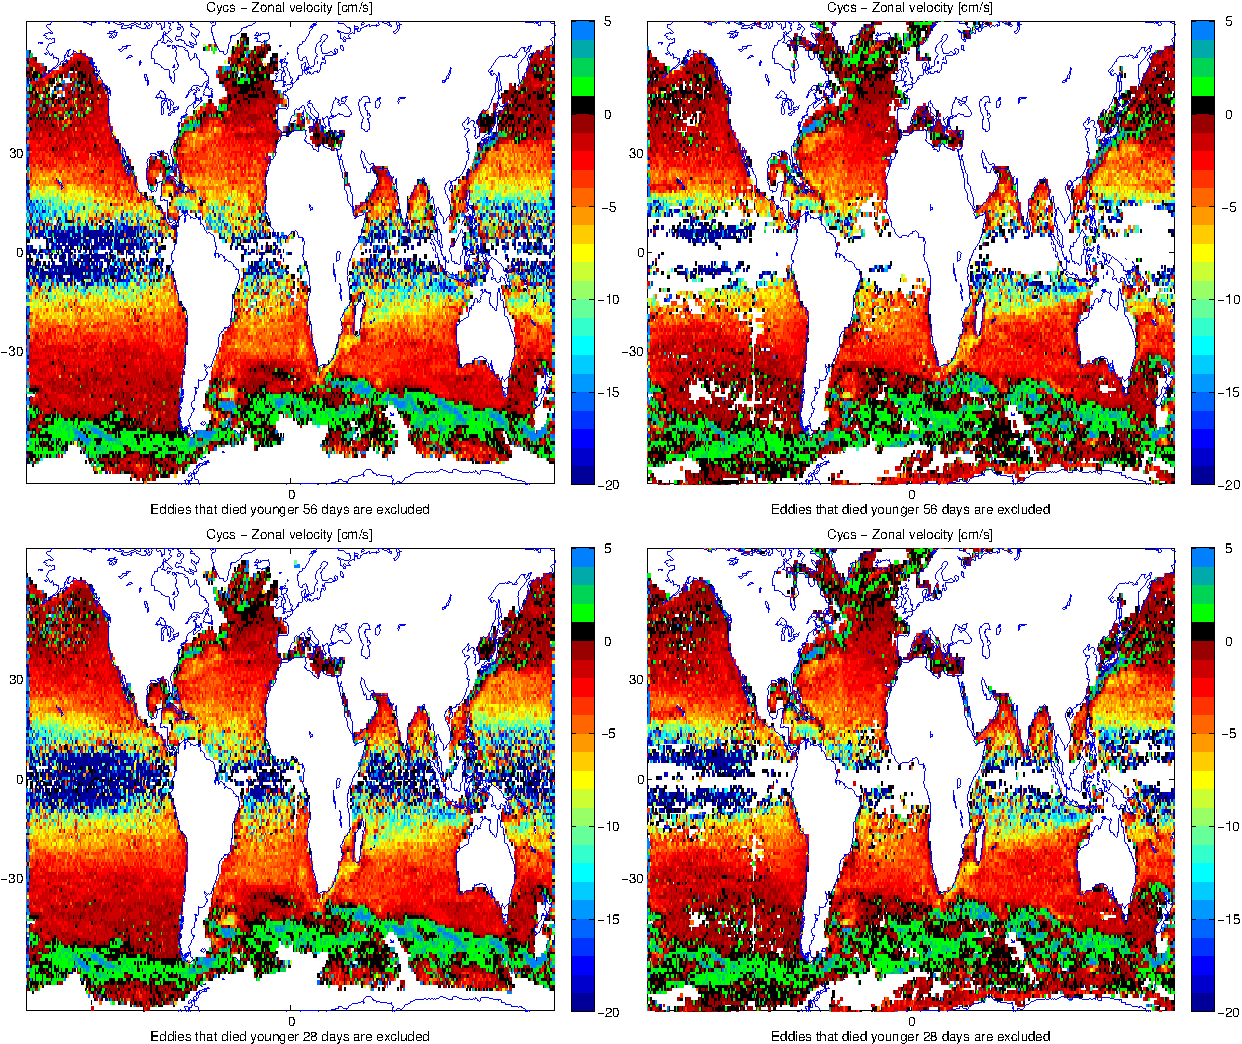
\includegraphics[height=220pt,keepaspectratio=true]{MUall.pdf}
	\end{figure}
\end{frame}

\begin{frame}
	\mtrx{zonal mean U}
	\begin{figure}
		\centering
		%\vspace{-10pt}
		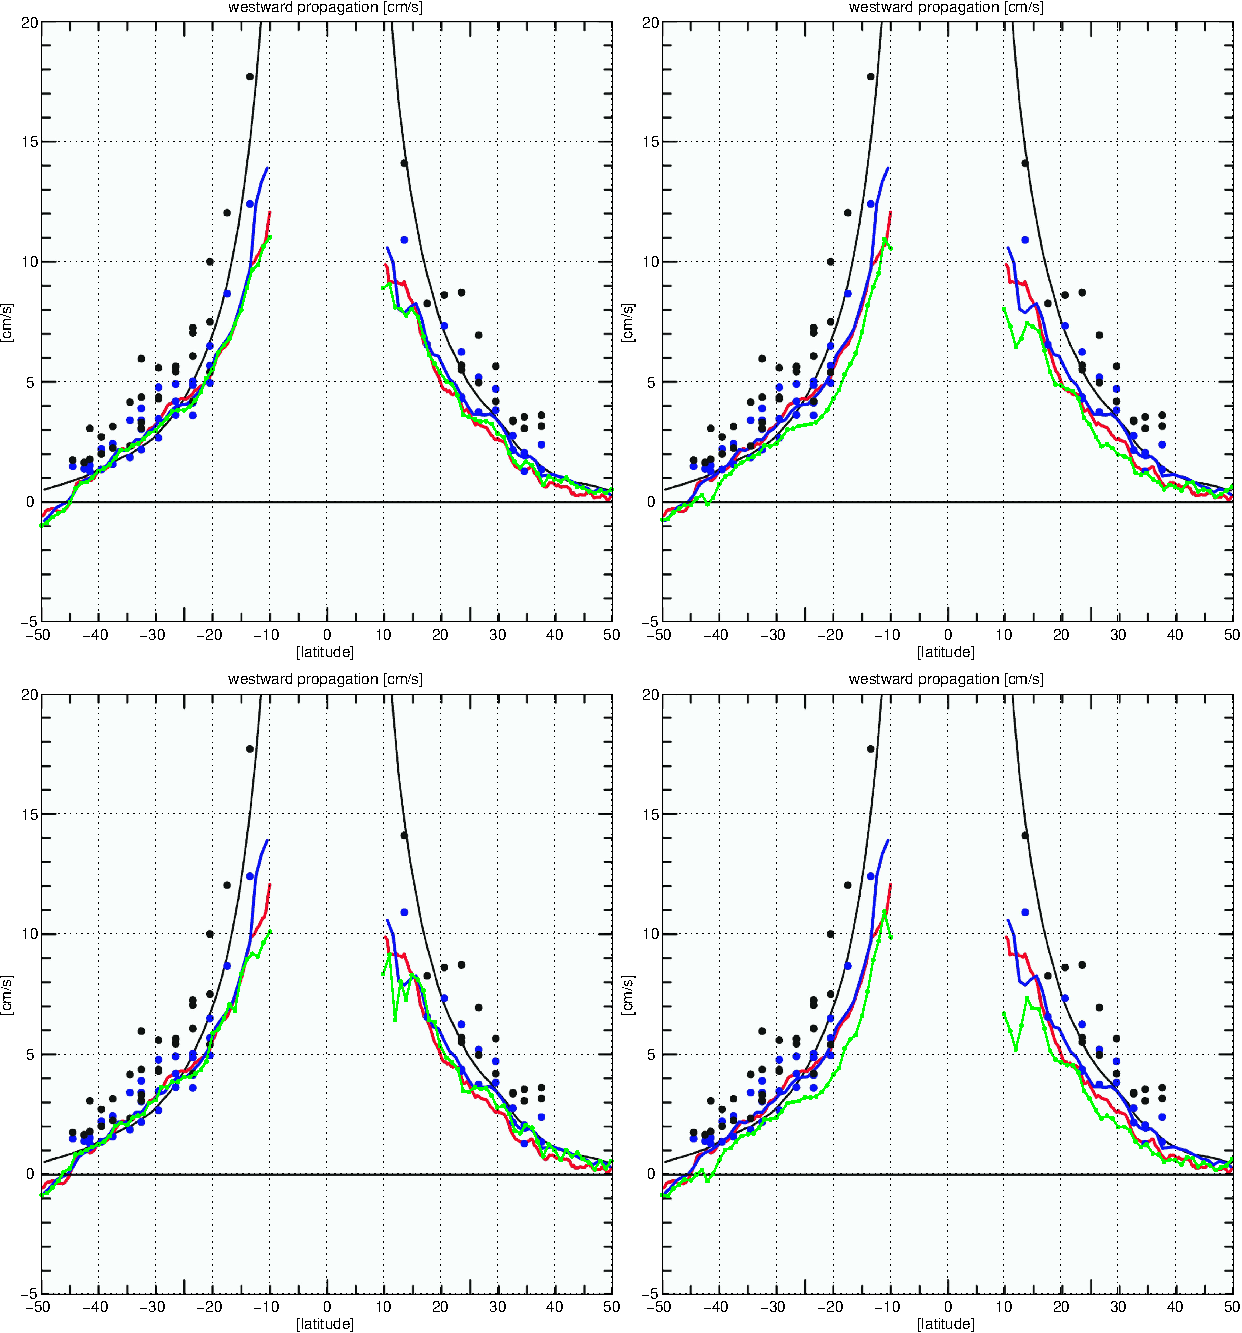
\includegraphics[height=210pt,keepaspectratio=true]{ZUall.pdf}
		\vspace{-10pt}
		\caption{
			\begin{tiny}
				 black dots: Radon transforms of 20°x10° high-pass filtered SSH fields along the 45 zonal sections. Red dots: means of $U$ along those sections (age $\ge 16$ weeks). red line: zonalmean(U). blue line: space-time-lagged cross-correlation (Fu 2009).
			\end{tiny}
		}
	\end{figure}
\end{frame}


\begin{frame}
\mtrx{$\sigma$}
 \begin{figure}
\centering
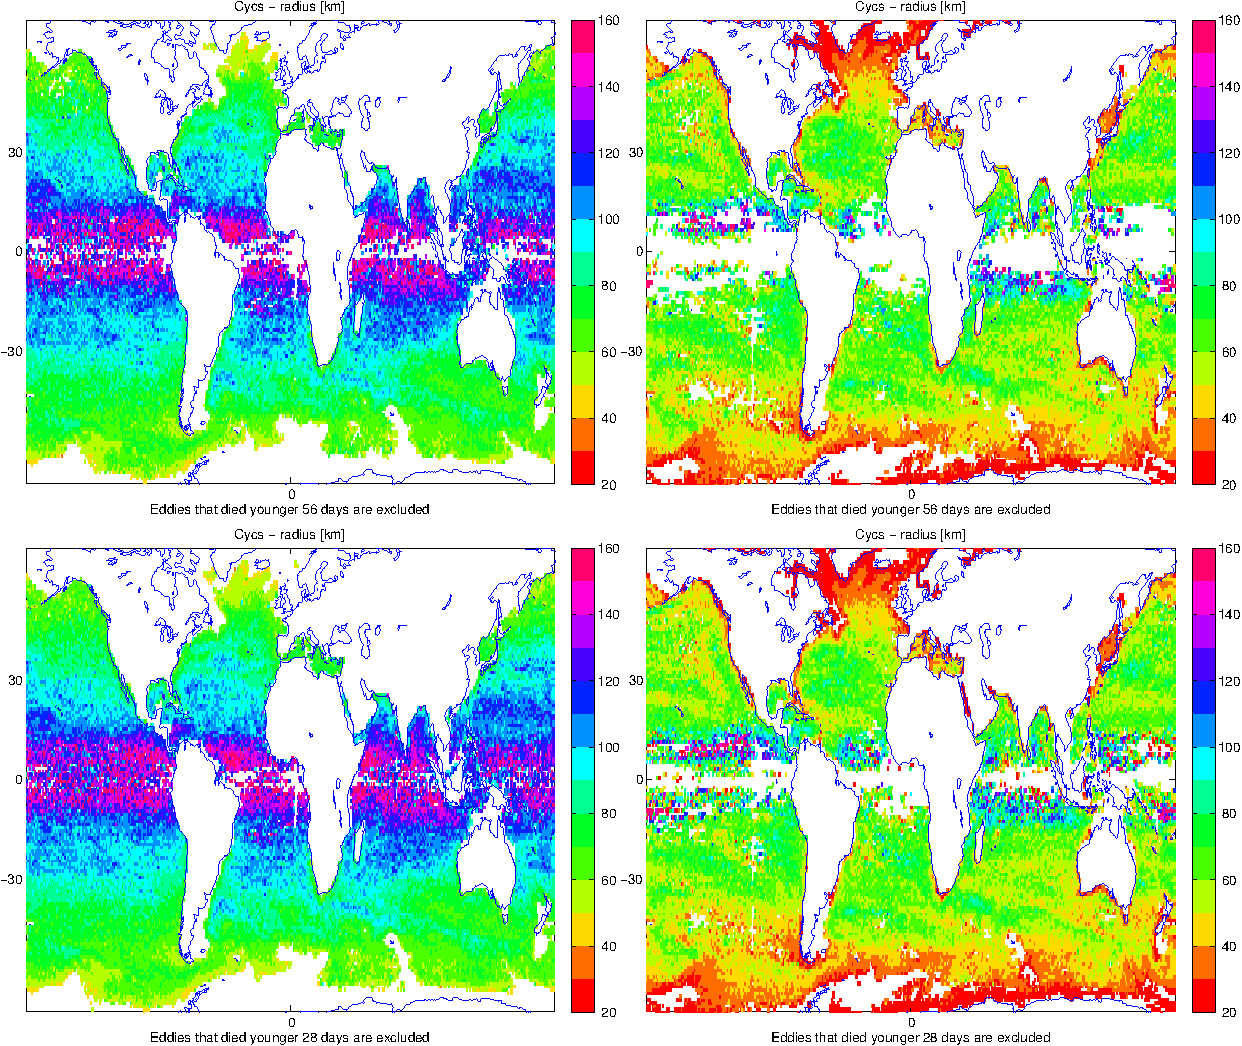
\includegraphics[height=220pt,keepaspectratio=true]{MRall.pdf}
\end{figure}
\end{frame}

\begin{frame}
\mtrx{zonal mean $\sigma$}
\begin{figure}
\centering
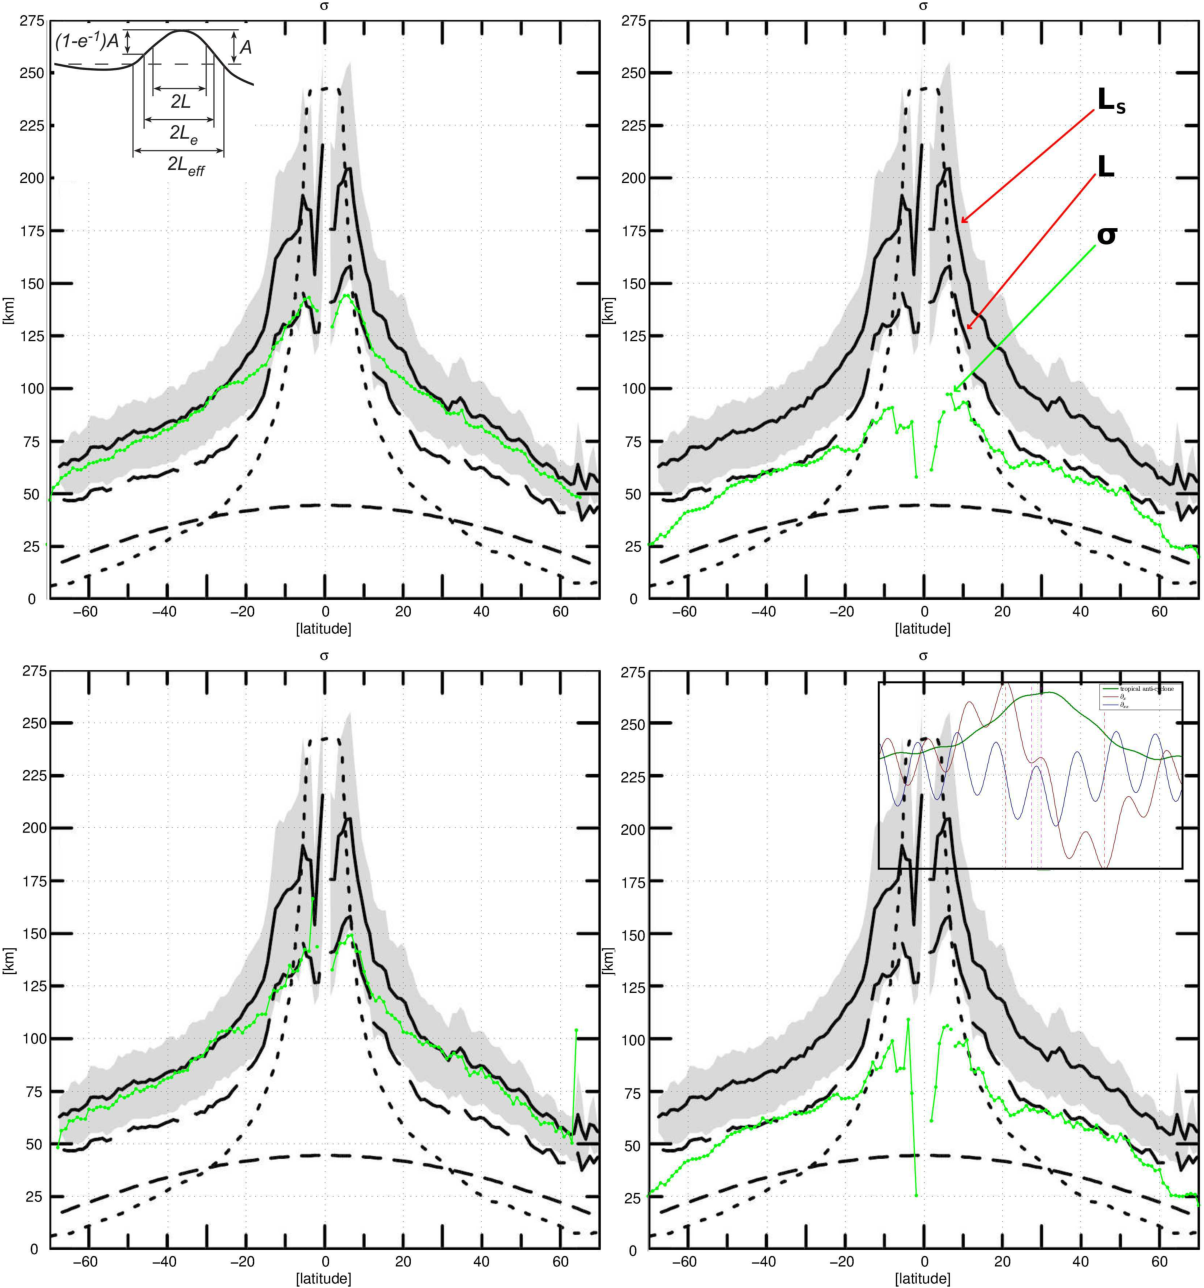
\includegraphics[height=220pt,keepaspectratio=true]{ZRall_anot.pdf}
\end{figure}
\end{frame}



\end{spacing}

%\section{next..}
%
%%
\newcommand{\cg}[1]{\cellcolor{green!25}#1}
\newcommand{\ce}[1]{\cellcolor{red!25}#1}
\newcommand{\cb}[1]{\cellcolor{gray!25}#1}
\newcommand{\n}{n/a}
\newcommand{\citeP}{\cite{Petersen2013}}
\newcommand{\citeCs}{\cite{Chelton2007}}
\newcommand{\citeCe}{\cite{Chelton2011}}
\newcommand{\citeCes}{\cite{Chelton2011,Chelton2007}}
\begin{frame}
 \frametitle{to-do-matrix}
 \begin{small} 
\begin{tabular}{r|c|c|c|}
\multicolumn{1}{c}{}	& \multicolumn{1}{c}{pop}	&	\multicolumn{1}{c}{aviso}	&	\multicolumn{1}{c}{comparison}\\
\cline{2-4}
U						&	\cg{\citeP}				&		\cg{\citeCes}			&		\cg{\citeP}	\\
\cline{2-4}
scale					&	\cg{\citeP}				&		\cg{\citeCes}			&		\cg{\citeP}	\\
\cline{2-4}
method Chelton			&	\ce{N}					&		\cg{\citeCe,N}			&		\ce{N}	\\
\cline{2-4}
method $R^2$			&	\cg{\citeP}				&		\cb{\n}					&		\cb{\n}	\\
\cline{2-4}
method OW				&	\cg{\citeP}				&		\cg{\citeCs}			&		\cg{\citeP}	\\
\cline{2-4}
method IQ				&	\ce{N}					&		\ce{N}					&		\ce{N}	\\
\cline{2-4}
net U					&	\ce{N}					&		\ce{N}					&		\ce{N}	\\
\cline{2-4}
steering level			&	\ce{N}					&		\cb{\n}					&		\cb{\n}	\\
\cline{2-4}
$p(z)$					&	\ce{N}					&		\cb{\n}					&		\cb{\n}	\\
\cline{2-4}
$f/H$					&	\ce{N}					&		\ce{ }					&		\ce{ }	\\
\cline{2-4}
remap pop2avi
&	\ce{ }					&		\ce{ }					&		\ce{ }	\\
\cline{2-4}
drop buoys into eddies
&	\ce{ }					&		\ce{ }					&		\ce{ }	\\
\cline{2-4}
go 3d
&	\ce{ }					&		\ce{ }					&		\ce{ }	\\
\cline{2-4}
\end{tabular}
\end{small}
\begin{tiny}
\bibliographystyle{acm}
\bibliography{/home/niko/documents/mendeley/library}
%\bibliography{/home/zmaw/u300065/mendeley/library}
\end{tiny}
\end{frame}


%\begin{frame}
%\bibliographystyle{acm}
%\bibliography{/home/zmaw/u300065/mendeley/library}
%\end{frame}


\begin{frame}
\frametitle{Which depth to take mean current from?}
\begin{figure}
	\centering
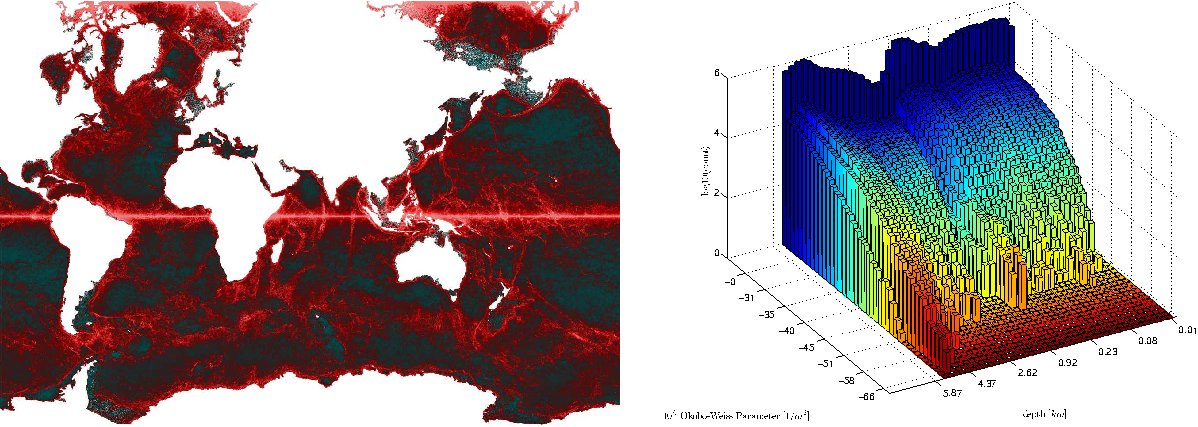
\includegraphics[width=330pt,keepaspectratio=true]{OWdouble.pdf}
\end{figure}
\end{frame}









\end{document}

% TODO umlaute

